% Copyright 2014 Jan-Philip Gehrcke

% http://www.howtotex.com/packages/the-nag-package-warns-you-for-incorrect-latex-usage/
\RequirePackage[l2tabu, orthodox]{nag}
\documentclass[a4paper,12pt,onecolumn,twoside,openright]{memoir}

% Use Linux Libertine font. A quote from Michael Sharpe: "The free font Linux
% Libertine is one particular target — it is of nearly the same x-height as
% Computer Modern, but, not being a modern font, does not have a high contrast
% ratio, and so appears denser than Computer Modern but not as much so as Times.
% It is meant as a replacement for Times, but differs from it in many
% characteristics, more similar to MinionPro than Times, and provides a better
% range of variants than Times — three weights (regular, semi-bold and bold)
% rather than just two, and has expert features in all weights: old-style
% figures, more extensive and more interesting ligatures, and small caps. In my
% opinion, material typeset in Linux Libertine looks better than the
% corresponding material typeset in Times. This seems especially true on the
% screen."

% Math font from newtx package, fits the Libertine text font very well.
% Must be loaded before fontspec, and fontspec must be loaded with the
% no-math option, followed by \usepackage{libertine} or
% \setmainfont{Linux Libertine O}, see
% http://tex.stackexchange.com/q/97299/11816
\usepackage[libertine]{newtxmath}
\usepackage[no-math]{fontspec}
\usepackage{libertine}

% Properly typeset units, and numbers with units.
\usepackage{siunitx}

% This is likely already loaded by some other package.
\usepackage{amsmath}

% Bold math symbols.
\usepackage{bm}

% Improve typography. Must be loaded after any font.
\usepackage{microtype}

% Dummy paragraphs.
\usepackage{lipsum}

\usepackage{graphicx}

% Highlight text via \hl{}.
\usepackage{soul}

% Temporary margin change.
%\usepackage[strict]{changepage}

% From my master thesis, will I use those?
\usepackage{booktabs}

% For SRED table in DMD chapter. TODO: Convert to not require that package.
\usepackage{threeparttable}

% insert other pdf documents
\usepackage{pdfpages}

\usepackage{url}

% captions (for figures etc)
%\DisemulatePackage{ccaption}
\usepackage[margin=5pt,font=small,labelfont=bf]{caption}

% Configure footnotes: counter reset every page etc.
\usepackage[perpage,hang,splitrule]{footmisc}

\usepackage[english]{babel}
\usepackage[babel]{csquotes}
\usepackage{color}
\usepackage{fancyvrb}
\usepackage{float}

% ftp://ftp.tu-chemnitz.de/pub/tex/macros/latex/contrib/nomencl/nomencl.pdf
% http://tex.stackexchange.com/a/100377
\usepackage[intoc]{nomencl}

% http://stackoverflow.com/a/8649145/145400 LaTeX won't hyphenate words with
% dashes in them. There's a standard package that addresses that very problem,
% called extdash. This defines new hyphen and dash commands that do not disrupt
% hyphenation, and which can allow or prevent line breaks at the hyphen/dash. I
% prefer to use it with the shortcuts option, so I can use, e.g., \-/ rather
% than \Hyphdash
\usepackage[shortcuts]{extdash}

% Intelligent space after "commands".
% http://tex.stackexchange.com/a/17873/11816
\usepackage{xspace}

% Add bibliography to ToC.
% http://en.wikibooks.org/wiki/LaTeX/Bibliography_Management
%\usepackage[nottoc]{tocbibind}

% Hyperref provides PDF links etc. Should be included as late as possible.
\usepackage{hyperref}

% See: Which packages should be loaded after hyperref instead of before?
% http://tex.stackexchange.com/q/1863

% This package introduces the \cref command. When using this command to make
% cross-references, instead of \ref or \eqref, a word is placed in front of the
% reference according to the type of reference: fig. for figures, eq. for
% equations.
% noabbrev option for non-abbreviated names.
\usepackage[noabbrev]{cleveref}


\definecolor{sepia}{cmyk}{0, 0.83, 1, 0.70}
\hypersetup{
    pdfauthor={Jan-Philip Gehrcke},
    pdftitle={Investigation of the interleukin-10-GAG interaction using molecular
        simulation methods},
    pdfsubject={PhD thesis, computational biophysics},
    pdfkeywords={one, two},
    colorlinks=true,
    linkcolor=sepia,
    citecolor=sepia,
    urlcolor=sepia
}

%\renewcommand{\unspace}{\relax}
% For styles, see
% ftp://ftp.rrzn.uni-hannover.de/pub/mirror/tex-archive/macros/latex/contrib/biblatex-contrib/
\usepackage[
    backend=biber,
    citestyle=numeric,
    %bibstyle=numeric,
    bibstyle=ieee,
    %citestyle=authoryear,
    %bibstyle=authoryear,
    hyperref=true,
    backref=true,
    sorting=none,
    indexing=true,
    sortcites=true,
    url=false,
    isbn=true,
    eprint=false,
    doi=true,
    ]{biblatex}

\addbibresource{literature.bib}
%\bibliography{literature}
%{\small\bibliography{literature.bib}}


% Footnote layout config
%\addtolength{\footskip}{0.5cm}
%\setlength{\footnotemargin}{0.2cm}
%\setlength{\footnotesep}{0.4cm}
%\makeatletter
%\let\splitfootnoterule=\pagefootnoterule
%\makeatother


% *************** Memoir page layout options ***************
\settypeblocksize{*}{\lxvchars}{1.618}
% First field: space between top page border and text.
\setulmargins{5cm}{*}{*}

% First field is "inner margin", defining the horizontal position of text block.
\setlrmargins{5cm}{*}{*}
%\setlrmargins{*}{*}{1.618}

%\setheadfoot{headheight}{footskip}
% footskip: text bottom to footer bottom
% headheight: height of header block
\setheadfoot{2\onelineskip}{2\onelineskip}

% Second field: space between text and header.
%\setheaderspaces{*}{2.5cm}{*}
\setheaderspaces{*}{4\onelineskip}{*}
\checkandfixthelayout


% *************** Chapter and section and head style ***************
%\chapterstyle{southall}
%\chapterstyle{veelo}
%\chapterstyle{bianchi}

% \setsecheadstyle{\Large\sffamily\bfseries}
% \setsubsecheadstyle{\large\sffamily\bfseries}
% \setsubsubsecheadstyle{\normalfont\sffamily\bfseries}
% \setparaheadstyle{\normalfont\sffamily}

% *************** Table of contents style ***************
%\settocdepth{section}
\setsecnumdepth{subsection}
\maxsecnumdepth{subsection}
\maxtocdepth{subsection}


% % ********** Commands for epigraphs **********
% \setlength{\epigraphwidth}{0.57\textwidth}
% \setlength{\epigraphrule}{0pt}
% \setlength{\beforeepigraphskip}{1\baselineskip}
% \setlength{\afterepigraphskip}{2\baselineskip}

% \newcommand{\epitext}{\sffamily\itshape}
% \newcommand{\epiauthor}{\sffamily\scshape ---~}
% \newcommand{\epititle}{\sffamily\itshape}
% \newcommand{\epidate}{\sffamily\scshape}
% \newcommand{\episkip}{\medskip}

% % temporal margin change
% % usage: \begin{changemargin}{-1cm}{-1cm}
% \newenvironment{changemargin}[2]{%
%  \begin{list}{}{%
%   \setlength{\topsep}{0pt}%
%   \setlength{\leftmargin}{#1}%
%   \setlength{\rightmargin}{#2}%
%   \setlength{\listparindent}{\parindent}%
%   \setlength{\itemindent}{\parindent}%
%   \setlength{\parsep}{\parskip}%
%  }%
% \item[]}{\end{list}}

% special hyphenation
% \hyphenation{na-no-par-ti-cles pe-rio-di-ci-ty T-pe-rio-di-ci-ty Lange-vin}
% \setlength{\emergencystretch}{1em}

% URL font style
% http://tex.stackexchange.com/a/109750/11816
\urlstyle{same}

% Define Angstrom command.
%\newcommand{\angstrom}{\textup{\AA}\xspace}
% http://tex.stackexchange.com/a/24282/11816
\sisetup{
    per-mode=symbol,
    text-angstrom={Å},
    math-angstrom={\text{Å}},
    separate-uncertainty,
    }
\DeclareSIUnit\calory{cal}

% Set smaller font size in bibliography.
\renewcommand*{\bibfont}{\small}

% http://tex.stackexchange.com/a/19678
\newcommand{\specialcell}[2][c]{%
  \begin{tabular}[#1]{@{}c@{}}#2\end{tabular}}

% A new float type 'listing' for presenting
% sourcecode.
\newfloat{listing}{tbph}{lop}[chapter]
\floatname{listing}{Listing}

% Date/Signature field
% http://tex.stackexchange.com/a/35943
\newcommand{\namesigdate}[2][5cm]{%
  \begin{tabular}{@{}p{#1}@{}}
    #2 \\[2\normalbaselineskip] \hrule \\[0pt]
    {\small \textit{Unterschrift}} \\[2\normalbaselineskip] \hrule \\[0pt]
    {\small \textit{Datum}}
  \end{tabular}
}


% ---- Definitions for Python code highlight BEGIN ----
% $ pygmentize -f latex -S default
\makeatletter
\def\PY@reset{\let\PY@it=\relax \let\PY@bf=\relax%
    \let\PY@ul=\relax \let\PY@tc=\relax%
    \let\PY@bc=\relax \let\PY@ff=\relax}
\def\PY@tok#1{\csname PY@tok@#1\endcsname}
\def\PY@toks#1+{\ifx\relax#1\empty\else%
    \PY@tok{#1}\expandafter\PY@toks\fi}
\def\PY@do#1{\PY@bc{\PY@tc{\PY@ul{%
    \PY@it{\PY@bf{\PY@ff{#1}}}}}}}
\def\PY#1#2{\PY@reset\PY@toks#1+\relax+\PY@do{#2}}

\expandafter\def\csname PY@tok@gd\endcsname{\def\PY@tc##1{\textcolor[rgb]{0.63,0.00,0.00}{##1}}}
\expandafter\def\csname PY@tok@gu\endcsname{\let\PY@bf=\textbf\def\PY@tc##1{\textcolor[rgb]{0.50,0.00,0.50}{##1}}}
\expandafter\def\csname PY@tok@gt\endcsname{\def\PY@tc##1{\textcolor[rgb]{0.00,0.27,0.87}{##1}}}
\expandafter\def\csname PY@tok@gs\endcsname{\let\PY@bf=\textbf}
\expandafter\def\csname PY@tok@gr\endcsname{\def\PY@tc##1{\textcolor[rgb]{1.00,0.00,0.00}{##1}}}
\expandafter\def\csname PY@tok@cm\endcsname{\let\PY@it=\textit\def\PY@tc##1{\textcolor[rgb]{0.25,0.50,0.50}{##1}}}
\expandafter\def\csname PY@tok@vg\endcsname{\def\PY@tc##1{\textcolor[rgb]{0.10,0.09,0.49}{##1}}}
\expandafter\def\csname PY@tok@m\endcsname{\def\PY@tc##1{\textcolor[rgb]{0.40,0.40,0.40}{##1}}}
\expandafter\def\csname PY@tok@mh\endcsname{\def\PY@tc##1{\textcolor[rgb]{0.40,0.40,0.40}{##1}}}
\expandafter\def\csname PY@tok@go\endcsname{\def\PY@tc##1{\textcolor[rgb]{0.53,0.53,0.53}{##1}}}
\expandafter\def\csname PY@tok@ge\endcsname{\let\PY@it=\textit}
\expandafter\def\csname PY@tok@vc\endcsname{\def\PY@tc##1{\textcolor[rgb]{0.10,0.09,0.49}{##1}}}
\expandafter\def\csname PY@tok@il\endcsname{\def\PY@tc##1{\textcolor[rgb]{0.40,0.40,0.40}{##1}}}
\expandafter\def\csname PY@tok@cs\endcsname{\let\PY@it=\textit\def\PY@tc##1{\textcolor[rgb]{0.25,0.50,0.50}{##1}}}
\expandafter\def\csname PY@tok@cp\endcsname{\def\PY@tc##1{\textcolor[rgb]{0.74,0.48,0.00}{##1}}}
\expandafter\def\csname PY@tok@gi\endcsname{\def\PY@tc##1{\textcolor[rgb]{0.00,0.63,0.00}{##1}}}
\expandafter\def\csname PY@tok@gh\endcsname{\let\PY@bf=\textbf\def\PY@tc##1{\textcolor[rgb]{0.00,0.00,0.50}{##1}}}
\expandafter\def\csname PY@tok@ni\endcsname{\let\PY@bf=\textbf\def\PY@tc##1{\textcolor[rgb]{0.60,0.60,0.60}{##1}}}
\expandafter\def\csname PY@tok@nl\endcsname{\def\PY@tc##1{\textcolor[rgb]{0.63,0.63,0.00}{##1}}}
\expandafter\def\csname PY@tok@nn\endcsname{\let\PY@bf=\textbf\def\PY@tc##1{\textcolor[rgb]{0.00,0.00,1.00}{##1}}}
\expandafter\def\csname PY@tok@no\endcsname{\def\PY@tc##1{\textcolor[rgb]{0.53,0.00,0.00}{##1}}}
\expandafter\def\csname PY@tok@na\endcsname{\def\PY@tc##1{\textcolor[rgb]{0.49,0.56,0.16}{##1}}}
\expandafter\def\csname PY@tok@nb\endcsname{\def\PY@tc##1{\textcolor[rgb]{0.00,0.50,0.00}{##1}}}
\expandafter\def\csname PY@tok@nc\endcsname{\let\PY@bf=\textbf\def\PY@tc##1{\textcolor[rgb]{0.00,0.00,1.00}{##1}}}
\expandafter\def\csname PY@tok@nd\endcsname{\def\PY@tc##1{\textcolor[rgb]{0.67,0.13,1.00}{##1}}}
\expandafter\def\csname PY@tok@ne\endcsname{\let\PY@bf=\textbf\def\PY@tc##1{\textcolor[rgb]{0.82,0.25,0.23}{##1}}}
\expandafter\def\csname PY@tok@nf\endcsname{\def\PY@tc##1{\textcolor[rgb]{0.00,0.00,1.00}{##1}}}
\expandafter\def\csname PY@tok@si\endcsname{\let\PY@bf=\textbf\def\PY@tc##1{\textcolor[rgb]{0.73,0.40,0.53}{##1}}}
\expandafter\def\csname PY@tok@s2\endcsname{\def\PY@tc##1{\textcolor[rgb]{0.73,0.13,0.13}{##1}}}
\expandafter\def\csname PY@tok@vi\endcsname{\def\PY@tc##1{\textcolor[rgb]{0.10,0.09,0.49}{##1}}}
\expandafter\def\csname PY@tok@nt\endcsname{\let\PY@bf=\textbf\def\PY@tc##1{\textcolor[rgb]{0.00,0.50,0.00}{##1}}}
\expandafter\def\csname PY@tok@nv\endcsname{\def\PY@tc##1{\textcolor[rgb]{0.10,0.09,0.49}{##1}}}
\expandafter\def\csname PY@tok@s1\endcsname{\def\PY@tc##1{\textcolor[rgb]{0.73,0.13,0.13}{##1}}}
\expandafter\def\csname PY@tok@sh\endcsname{\def\PY@tc##1{\textcolor[rgb]{0.73,0.13,0.13}{##1}}}
\expandafter\def\csname PY@tok@sc\endcsname{\def\PY@tc##1{\textcolor[rgb]{0.73,0.13,0.13}{##1}}}
\expandafter\def\csname PY@tok@sx\endcsname{\def\PY@tc##1{\textcolor[rgb]{0.00,0.50,0.00}{##1}}}
\expandafter\def\csname PY@tok@bp\endcsname{\def\PY@tc##1{\textcolor[rgb]{0.00,0.50,0.00}{##1}}}
\expandafter\def\csname PY@tok@c1\endcsname{\let\PY@it=\textit\def\PY@tc##1{\textcolor[rgb]{0.25,0.50,0.50}{##1}}}
\expandafter\def\csname PY@tok@kc\endcsname{\let\PY@bf=\textbf\def\PY@tc##1{\textcolor[rgb]{0.00,0.50,0.00}{##1}}}
\expandafter\def\csname PY@tok@c\endcsname{\let\PY@it=\textit\def\PY@tc##1{\textcolor[rgb]{0.25,0.50,0.50}{##1}}}
\expandafter\def\csname PY@tok@mf\endcsname{\def\PY@tc##1{\textcolor[rgb]{0.40,0.40,0.40}{##1}}}
\expandafter\def\csname PY@tok@err\endcsname{\def\PY@bc##1{\setlength{\fboxsep}{0pt}\fcolorbox[rgb]{1.00,0.00,0.00}{1,1,1}{\strut ##1}}}
\expandafter\def\csname PY@tok@kd\endcsname{\let\PY@bf=\textbf\def\PY@tc##1{\textcolor[rgb]{0.00,0.50,0.00}{##1}}}
\expandafter\def\csname PY@tok@ss\endcsname{\def\PY@tc##1{\textcolor[rgb]{0.10,0.09,0.49}{##1}}}
\expandafter\def\csname PY@tok@sr\endcsname{\def\PY@tc##1{\textcolor[rgb]{0.73,0.40,0.53}{##1}}}
\expandafter\def\csname PY@tok@mo\endcsname{\def\PY@tc##1{\textcolor[rgb]{0.40,0.40,0.40}{##1}}}
\expandafter\def\csname PY@tok@kn\endcsname{\let\PY@bf=\textbf\def\PY@tc##1{\textcolor[rgb]{0.00,0.50,0.00}{##1}}}
\expandafter\def\csname PY@tok@mi\endcsname{\def\PY@tc##1{\textcolor[rgb]{0.40,0.40,0.40}{##1}}}
\expandafter\def\csname PY@tok@gp\endcsname{\let\PY@bf=\textbf\def\PY@tc##1{\textcolor[rgb]{0.00,0.00,0.50}{##1}}}
\expandafter\def\csname PY@tok@o\endcsname{\def\PY@tc##1{\textcolor[rgb]{0.40,0.40,0.40}{##1}}}
\expandafter\def\csname PY@tok@kr\endcsname{\let\PY@bf=\textbf\def\PY@tc##1{\textcolor[rgb]{0.00,0.50,0.00}{##1}}}
\expandafter\def\csname PY@tok@s\endcsname{\def\PY@tc##1{\textcolor[rgb]{0.73,0.13,0.13}{##1}}}
\expandafter\def\csname PY@tok@kp\endcsname{\def\PY@tc##1{\textcolor[rgb]{0.00,0.50,0.00}{##1}}}
\expandafter\def\csname PY@tok@w\endcsname{\def\PY@tc##1{\textcolor[rgb]{0.73,0.73,0.73}{##1}}}
\expandafter\def\csname PY@tok@kt\endcsname{\def\PY@tc##1{\textcolor[rgb]{0.69,0.00,0.25}{##1}}}
\expandafter\def\csname PY@tok@ow\endcsname{\let\PY@bf=\textbf\def\PY@tc##1{\textcolor[rgb]{0.67,0.13,1.00}{##1}}}
\expandafter\def\csname PY@tok@sb\endcsname{\def\PY@tc##1{\textcolor[rgb]{0.73,0.13,0.13}{##1}}}
\expandafter\def\csname PY@tok@k\endcsname{\let\PY@bf=\textbf\def\PY@tc##1{\textcolor[rgb]{0.00,0.50,0.00}{##1}}}
\expandafter\def\csname PY@tok@se\endcsname{\let\PY@bf=\textbf\def\PY@tc##1{\textcolor[rgb]{0.73,0.40,0.13}{##1}}}
\expandafter\def\csname PY@tok@sd\endcsname{\let\PY@it=\textit\def\PY@tc##1{\textcolor[rgb]{0.73,0.13,0.13}{##1}}}

\def\PYZbs{\char`\\}
\def\PYZus{\char`\_}
\def\PYZob{\char`\{}
\def\PYZcb{\char`\}}
\def\PYZca{\char`\^}
\def\PYZam{\char`\&}
\def\PYZlt{\char`\<}
\def\PYZgt{\char`\>}
\def\PYZsh{\char`\#}
\def\PYZpc{\char`\%}
\def\PYZdl{\char`\$}
\def\PYZhy{\char`\-}
\def\PYZsq{\char`\'}
\def\PYZdq{\char`\"}
\def\PYZti{\char`\~}
% for compatibility with earlier versions
\def\PYZat{@}
\def\PYZlb{[}
\def\PYZrb{]}
\makeatother
% ---- Definitions for Python code highlight END ----

% Declare hyphenation rules for certain words (these rules take global effect).
% The \hyphenation command allows you to give explicit instructions. Provided
% that the word will hyphenate at all (that is, it is not prevented from
% hyphenating by any of the other restrictions above), the command will override
% anything the hyphenation patterns might dictate. The command takes one or more
% hyphenated words as argument — \hyphenation{ana-lysis pot-able}; note that (as
% here, for analysis) you can use the command to overrule TeX’s choice of
% hyphenation
\hyphenation{
    he-xa-sac-cha-ride
    mo-no-sac-cha-ride
    di-sac-cha-ride
    te-tra-sac-cha-ride
    ace-tyl-glu-co-sa-mine
    }

% http://tex.stackexchange.com/a/100377
\makenomenclature

\begin{document}

% Include PDF pages created externally (title page etc).
% http://tu-dresden.de/die_tu_dresden/fakultaeten/fakultaet_mathematik_und_naturwissenschaften/deckblatt_dissertation
% Disable hyperref links for these pages, to prevent page identifier collision.
% http://tex.stackexchange.com/a/18927/11816
% Page identifier collision still happens, without affecting final document.
% Relevant error message:
% [3]LuaTeX warning (ext4): destinat ion with the same identifier (name{page.4})
% has been already used, duplicate ignored
\hypersetup{pageanchor=false}

\includepdf{pdf_pages_for_inclusion/titlepage_01.pdf}

% Start on recto page.
\cleardoublepage


\includepdf{pdf_pages_for_inclusion/logopage_01.pdf}
\hypersetup{pageanchor=true}

% The \frontmatter declaration sets the folios to be printed in lowercase roman
% numerals, starts the page numbering from i, and prohibits any numbering of
% sectional divisions. Caption, equations, etc., will be numbered continuously.
\frontmatter

\chapter{Introduction and summary}
% Abgegeben werden muss, according to Promotionsordnung:
% 3. eine Dissertation in 4 Exemplaren, maschinenschriftlich und gebunden sowie
%15 Exemplare einer Kurzfassung (maximal drei Seiten);

% Das hier ist sowohl die interne als auch die externe Kurzfassung.


Glycosaminoglycans (GAGs) are a class of linear polysaccharides, built of
periodically occurring disaccharide units. GAGs are ubiquitous in the
extracellular matrix (ECM), where they exhibit multifarious biological
activities. This diversity arises from --- among others --- their ability to
interact with and regulate a large number of proteins, such as cytokines,
chemokines, and growth factors. As of the huge variety in their chemical
configuration, GAGs are further sub-classified into different types of GAGs
(heparin, for instance, is one of these sub-classes). Hence, GAGs are a
\textit{diverse} class of molecules, which surely contributes to the broadness
of their spectrum of biological functions. Through varying arrangements of
sulfate groups and different types of monosaccharides, individual GAG molecules
can establish highly specific atomic contacts to certain proteins. One of the
best-studied examples is antithrombin-heparin, whose biologically relevant
interaction requires a specific pentasaccharide sequence
\cite{antithrombin-thrombin-heparin-2004}. It is valid to assume, however, that
various proteins are yet to be discovered whose biological function is in some
way affected by GAGs. In other cases, and this is true for the cytokine
interleukin-10 (IL-10), there are already experimental clues for a biologically
relevant protein-GAG interaction, but the details are still obscure and the
fundamental molecular interaction mechanism has still not been clarified.

IL-10 has been shown to bind certain GAGs \cite{salek_ardakani_2000}. So far,
however, no structural detail about IL-10-GAG interaction is known.
Function-wise, IL-10 is mainly considered to be immunosuppressive and therefore
anti-inflammatory, but it in fact has the pleiotropic ability to influence the
immune system in both directions, i.e.\ it constitutes a complex regulation
system on its own. Therefore, the role of GAGs in this system is potentially
substantial, but is yet to be clarified. \textit{In vitro} experiments have
yielded indications for GAGs being able to modulate IL-10's biological function
\cite{salek_ardakani_2000}, and obviously IL-10 and GAGs are simultaneously
present in the ECM. This gives rise to the assumption that IL-10-GAG interaction
is of biological significance, and that understanding the impact of GAGs on
IL-10 biology is important --- from the basic research point of view, but also
for the development of therapeutic approaches. A promising approach for
obtaining knowledge about the nature of IL-10-GAG interaction is the
investigation of this system on the structural level, i.e.\ the identification
and characterization of the molecular interaction mechanisms that govern the
IL-10-GAG system.

In this PhD project it was my goal to reveal structural and molecular details
about IL-10-GAG interaction with theoretical and computational means, and with
the help of experiments performed by collaborators. In the course of the
project, three methods were developed for the \textit{in silico} investigation
of protein-GAG complexes and subsequently applied them to the IL-10-GAG system.

I proposed and validated a systematic approach for predicting GAG binding
regions on a given protein, based on the numerical simulation and analysis of
the Coulomb potential of the protein. One major advantage of this method is its
intrinsic ability to assess the reliability of the resulting prediction. In case
of IL-10, the application of this method lead to the observation that its
Coulomb attraction for GAGs is significantly weaker than in case of exemplary
protein-GAG systems (such as FGF2-heparin). Still, a distinct IL-10-GAG binding
region centered on the residues R102, R104, R106, R107 of the human IL-10
monomer was identified, and this region can be assumed to play a major role in
IL-10-GAG interaction, as described in \cref{chapter:bspred}.

Molecular docking methods are often used to generate a binding mode prediction
for a given receptor-ligand system. In \cref{chapter:clustering}, I clarify the
importance of data clustering as an essential step for post-processing an
ensemble of docking solutions. In the course of the PhD project, I developed a
clustering methodology optimized for GAG molecules. It allows for a reproducible
analysis, enabling systematic comparisons among different docking studies. This
clustering approach has become standard procedure in the Pisabarro research
group. It has so far been used in a variety of published studies (e.g.
\cite{franz_cathepsin_2013}), and also played an important role in the
investigation of the IL-10-GAG system, as described in \cref{chapter:dmdil10} of
this thesis.

Motivated by the shortcomings of classical docking approaches, especially with
respect to protein-GAG systems, we (a colleague of mine and I) developed a
molecular dynamics-based docking method with less radical approximations than
usually applied in classical docking. The goal was to make the computational
model properly account for the special physical properties of GAGs, and to
especially include the effects of flexibility and solvation. We named the method
Dynamic Molecular Docking (DMD), and successfully published its concept together
with a validation study \cite{dmd_samsonov_gehrcke_2014}. The following
application of DMD in a variety of studies required enormous amounts of
computational resources. For tackling this challenge, I established a graphics
processing unit-based high performance computing (HPC) environment in our
research group and developed a software framework for reliably performing DMD
studies on this hardware, as well as on other HPC resources of the TU Dresden.

The subsequent investigation of the IL-10-GAG system via DMD was focused on the
IL-10-GAG binding region predicted earlier, and made heavy usage of the
optimized clustering approach. An important result of this endeavor is that
IL-10's amino acid residue R107 significantly stands out compared to all other
residues and supposedly plays a particularly important role in IL-10-GAG
recognition.

Furthermore, the collaboration with the NMR laboratory of Prof. Daniel Huster at
University Leipzig was fruitful: I post-processed nuclear Overhauser effect data
and obtained GAG structure models, which revealed that IL-10-heparin interaction
has a measurable impact on the backbone structure of the heparin molecule. These
results were published in \cite{kuenze_gehrcke_2014}.

\hl{Crystal structure sulfate groups, ternary receptor model, binding region
prediction, lead to models that might explain the role of IL-10-GAG interaction
in IL-10 biology...}.

In conclusion, valuable information for deepening the understanding of the
molecular mechanism governing IL-10-GAG interaction have been derived. These
observations pave the further way towards unraveling GAG-mediated bioactivity of
IL-10, which may then be specifically exploited, for instance in artificial
extracellular matrices for improved wound healing. Furthermore, various methods
have been developed which are generically applicable for the investigation of
protein-GAG systems.


% IIRC, the adjustwidth env is defined by memoir.
\begin{adjustwidth}{-1.5cm}{-1.5em}
\tableofcontents
\end{adjustwidth}

% Mainmatter changes page numbering etc, see memoir docs.
\mainmatter
\pagestyle{Ruled}
\makeoddhead{Ruled}{}{}{\small\sffamily\bfseries\rightmark}
\chapter{Background}
\label{background}

\section{Glycosaminoglycans (GAGs)}
\label{background:gags}


\subsubsection{General aspects}%The nature of GAGs}
Carbohydrates are ubiquitous building blocks found in all forms of life. As
implicated by their name, they are made of carbon, hydrogen and oxygen. Despite
this rather small set of atom types, an enormous variety of carbohydrates
exists. The origin of major parts of this diversity is of combinatorial nature:
carbohydrates usually occur as polysaccharides made of many connected
monosaccharides (or \enquote{sugar rings}), whereas various different types of
monosaccharides are available in nature. They are distinguishable by their
chemical configuration, and usually there are two stereoisomers for each of
those configurations, leading to a broad spectrum of different sugar rings whose
nomenclature and chemistry are described in detail in reference books
\cite{carbohydrate_chemistry_robyt_1998, carbohydrate_chemistry_royal_2000}.
Glycosaminoglycans (GAGs), reviewed in
\cite{essentials_glycobiology_gags_chapter_2009}, are a special class of
carbohydrates. GAGs play a critical role in many biological processes; they are
important for cell adhesion and cell growth, and their multifarious biological
activity arises from their ability to interact with and regulate a large number
of proteins \cite{handel_2005,gandhi_structure_2008}. Likewise, both natural and
artificial GAGs are promising tools for therapies, for instance for the design
of new bio-materials for the use in the field of regenerative medicine
\cite{whitelock_2014,schnabelrauch_tissues_2013,scott_gags_therapies_2013}.

GAGs are unbranched (linear) saccharide chains, comprised of a periodically
repeating unit, whereas each unit is made of two pyranose (a six-membered ring
consisting of five carbon atoms and one oxygen atom) monosaccharides:

\nomenclature{GAG}{glycosaminoglycan}

\begin{itemize}
\item One is an amino sugar or \enquote{hexosamine}, either a
D\-/N\-/acetylglucosamine (GlcN) or a D\-/N\-/acetylgalactosamine (GalN).
\item The other is a uronic saccharide or \enquote{hexuronic acid}, either a
D-glucuronic acid (GlcA) or its C5\-/epimer L\-/iduronic acid (IdoA), or, in
seldom cases, a D\-/galactose (Gal).
\end{itemize}


\nomenclature{IdoA}{L-iduronic acid}
\nomenclature{GlcA}{D-glucuronic acid}
\nomenclature{GalN}{D-N-acetylgalactosamine}
\nomenclature{GlcN}{D-N-acetylglucosamine}


\begin{table}
\scriptsize
\centering
\renewcommand{\arraystretch}{1.3}
\begin{tabular}{lll}
\midrule
GAG type & main disaccharide & charge/\si{\elementarycharge} \\
\midrule
Heparin (HP) & L-IdoA2S-$\alpha$(1$\rightarrow$4)-D-GlcNS6S-$\alpha$(1$\rightarrow$4) & -4 \\
Chondroitin-4-sulfate (CS4) & D-GlcA-$\beta$(1$\rightarrow$3)-D-GalN4S-$\beta$(1$\rightarrow$4) & -2 \\
Hyaluronan (HA) & D-GlcA-$\beta$(1$\rightarrow$4)-D-GlcN-$\alpha$(1$\rightarrow$4) & -1 \\
\midrule
\end{tabular}
\caption{
Fundamentally different GAG types, their repeating disaccharide unit in IUPAC
nomenclature, and their charge per disaccharide, in units of the elementary
charge. The abbreviations given in brackets in the first column are used
throughout this thesis.}
\label{tab:bg:gagtypes}
\end{table}

\nomenclature{HP}{heparin}
\nomenclature{HA}{hyaluronan}
\nomenclature{CS4}{chondroitin-4-sulfate}
\nomenclature{CS6}{chondroitin-6-sulfate}
\nomenclature{HS}{heparan sulfate}

A special feature of GAGs is that they are usually sulfated at various ring
positions, leading to a number of possible sulfation patterns per repeating
disaccharide unit. The number of possible combinations of basic disaccharide
units, two different allowed geometries of the glycosidic linkage between them,
and variations in the sulfation pattern imply that the heterogeneity among GAGs
is large. Still, physiologically occurring GAGs can be roughly categorized into
six major GAG types. Three of those, the most important ones for this thesis,
are listed in \cref{tab:bg:gagtypes} together with their repeating disaccharide
unit, sulfation pattern, glycosidic linkage type, and with their abbreviation
used here from now on. Three other major GAG types are usually listed in
literature \cite{gandhi_structure_2008}, which play a less important role in
this thesis than the ones listed in \cref{tab:bg:gagtypes}:

\begin{itemize}
\item Heparan sulfate, which is considered to be an analogue of heparin. The
only difference is that heparan sulfate has --- on average --- a higher content
of glucuronic acid than iduronic acid.
\item Dermatan sulfate, which is similar to chondroitin sulfate, but is built of
iduronic acid instead of glucuronic acid.
\item Keratan sulfate, the only GAG type that contains a D\-/galactose
saccharide instead of an acid. The amino sugar is the same as in chondroitin
sulfate.
\end{itemize}

Except for HA, which is the only non-sulfated GAG, the naturally occurring
sulfation of GAGs is strong, with up to three sulfate groups per disaccharide
unit in case of heparin. Considering the carboxyl group contained in the
hexuronic acid, each repeating disaccharide unit always carries at least one
negative charge at physiological pH (which is also true for HA). Adding
sulfation, this charge may grow up to -4 for heparin (see
\cref{tab:bg:gagtypes}), which in fact is the biological macromolecule with the
largest charge density known \cite{capila_linhardt_hep_prot_2002}.
\Cref{fig:bg:heparin_chemstruct} shows the chemical configuration of the
repeating disaccharide unit of heparin and schematically visualizes its
structure in space. What is depicted there actually is the disaccharide unit
which occurs \textit{most frequently} in natural heparin polysaccharides.
Polymeric GAGs in an organism can be quite long with a molecular weight of about
10 to 100\,kDa \cite{gandhi_structure_2008}, and they never reach
\SI{100}{\percent} purity. That is, natural GAGs are always comprised of a
mixture of more than only two monosaccharides, and the repeating units shown in
\cref{tab:bg:gagtypes} are the \textit{dominating} ones for each of the cases.

\begin{figure}
\centering
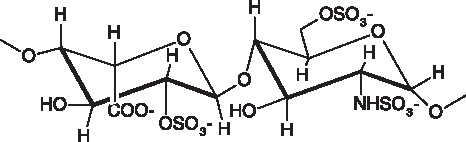
\includegraphics[width=1.0\textwidth]{gfx/background/hp_repeating_unit_structure_01.pdf}
\caption[]{
Molecular configuration of the repeating disaccharide unit of heparin (the one
which occurs most frequently in natural heparin polysaccharides). The pyranose
to the left is a 2-O-sulfated iduronic acid (IdoA2S), connected via a
1$\rightarrow$4 glycosidic linkage to the 6-O-sulfated
2-deoxy-2-sulfamido-α-D-N\-/acetylglucosamine (GlcNS6S). At physiological pH,
the charge of this disaccharide is -4 elementary charges.
}
\label{fig:bg:heparin_chemstruct}
\end{figure}

There are many more than six GAG variants with established names, such as
Chondroitin\-/6\-/sulfate (CS6), which is the same as CS4, but sulfated at the
C6 position of the galactosamine instead of in the fourth position. With the GAG
types described here so far, all major characteristics of naturally occurring
GAG molecules are covered. Other GAG types are not listed, because they are not
fundamentally different from what has been described and therefore were not
investigated in the framework of this thesis.

In organisms, all GAG chains except for HA  appear covalently bound to a core
protein, comprising a so-called \textit{proteoglycan} complex
\cite{essentials_glycobiology_gags_chapter_2009}. These large structures consist
of a linear protein with many GAGs covalently linked to it. Each GAG is linked
to the core protein via a special sugar linker, which itself is attached to
(usually) a serine residue of the core protein. As of the length of the GAG
chains, however, the biological functions of proteoglycans depend to a large
extent only on the interaction of its GAG chain(s) with other proteins, i.e.\
the free end of a GAG chain can be considered unaffected by the core protein.
This is one of the fundamental assumptions applied in this thesis project: GAGs
are considered and treated as \textit{free} molecules.



%While it is likely
%that their tremendous length and also their covalent linkage to proteoglycans
%serve have an overall impact on the biological function of GAGs, it is a
%valid and well-established approximation to not account for these facts in
%molecular modeling studies that aim for resolving the molecular mechanism of
%protein-GAG interaction in atomic detail... in a biological function and overall  treated as


\subsubsection{Pyranose conformations}
\label{background:gags:conformations}

The origin and geometry of various pyranose monosaccharide conformations is
comprehensibly classified and discussed in
\cite{classification_pyranose_conformers_1960}. The conformational nomenclature
used throughout this thesis follows IUPAC rules, which are well-described in
\cite{iupac_gag_conformations_1980}.

Free in solution, most monosaccharide rings in GAGs have one clearly predominant
conformation, and their ring structure can therefore be considered
\textit{rigid}, as is the case for e.g.\ D-glucuronic acid (GlcA), which resides
in a stable ${}^{4}\mathrm{C}_1$ chair \cite{almond_jacs_2010}. Also
N-acetyl-D-glucosamine (GlcN) mainly populates the ${}^{4}\mathrm{C}_1$ ring
conformation, which was shown to be especially stable when the GlcN becomes
sulfated \cite{Sattelle_glcnac_right_chair_2011}, as is the case in heparin. The
pyranose ring of iduronic acid (IdoA), a constituent of heparin, however, is the
only GAG pyranose that is --- free in solution, i.e.\ without any mechanical
stress --- in an equilibrium of multiple so-called ring puckers. C5 carboxyl
epimerization is the the only difference of IdoA compared to GlcA, and it
results in conformational instability. IdoA is postulated to be populated by a
mixture of mainly three conformations \cite{almond_jacs_2010}:
${}^{4}\mathrm{C}_1$, ${}^{1}\mathrm{C}_4$, and ${}^{2}\mathrm{S}_\mathrm{O}$.
Obviously, this conformational flexibility of IdoA is a \textit{structural
flexibility} which allows for different orientations of functional groups in
space, as depicted in \cref{fig:bg:idoa_conformations}.

\begin{figure}
\centering
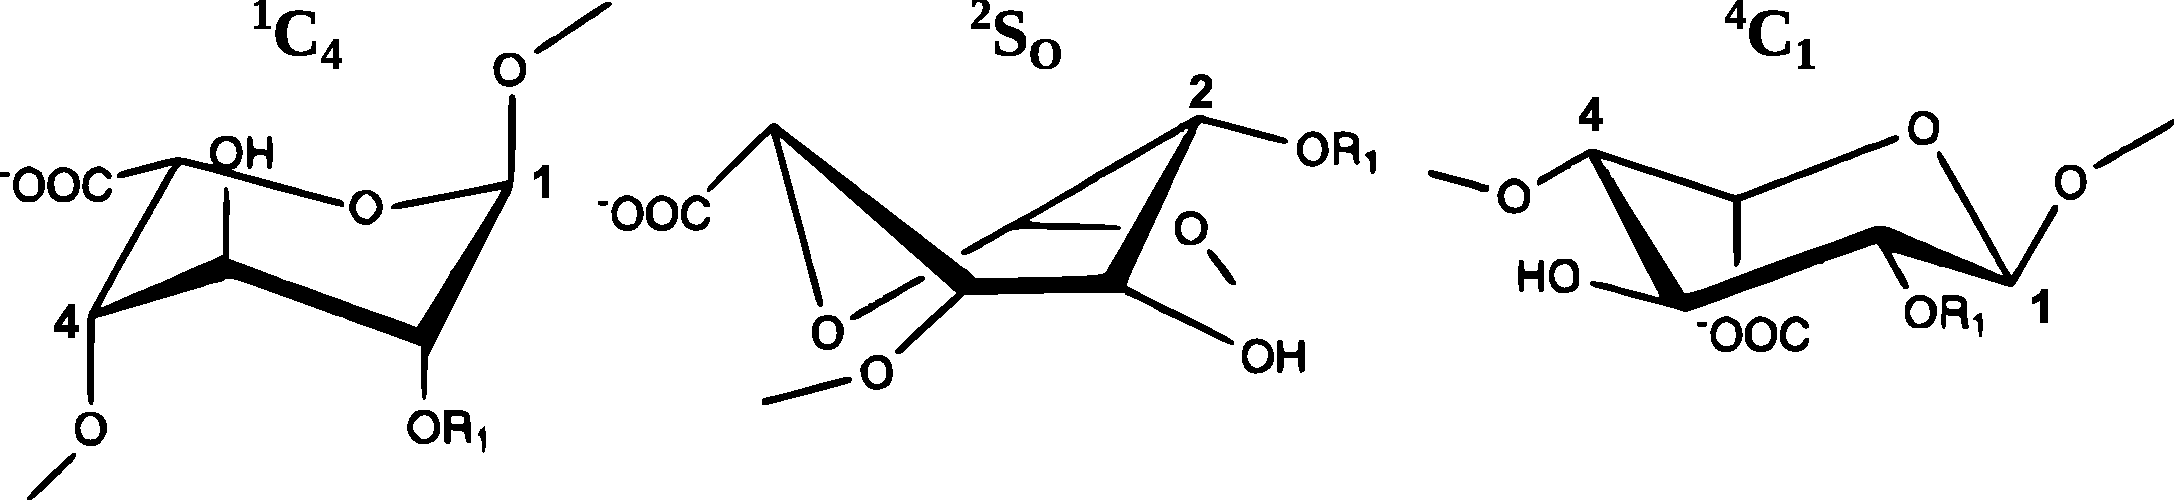
\includegraphics[width=1.0\textwidth]{gfx/background/idoa_conformations_03.pdf}
\caption[]{
The three conformations (two chairs, one skew-boat) of the pyranose L-iduronic
acid which are most populated in solution. In heparin, $\mathrm{R}_1$ is a
sulfate group.}
\label{fig:bg:idoa_conformations}
\end{figure}


The exact population ratios and exchange time scales of the conformations of
IdoA are difficult to measure and simulate \cite{almond_jacs_2010,
structure_gags_progess_perspectives_2010}, but they clearly depend on the IdoA
environment. That is, a terminal IdoA behaves differently from an IdoA pyranose
within a GAG chain. As shown by Sattelle et al., the population ratio depends on
sulfation, and IdoA2S still prevails in an equilibrium of multiple highly
populated conformations \cite{almond_jacs_2010}. Regarding heparin-internal
IdoA2S, Muñoz-García and co-workers summarize that it is in an equilibrium of
${}^{2}\mathrm{S}_\mathrm{O}$ and ${}^{1}\mathrm{C}_4$ with a negligible content
of the ${}^{4}\mathrm{C}_1$ chair \cite{conf_idoa_timeavg_restraints_2013}. The
interconversion between ${}^{2}\mathrm{S}_\mathrm{O}$ and ${}^{1}\mathrm{C}_4$
has earlier been described to exert only little geometrical change on glycosidic
linkages \cite{Mulloy_dyn_conf_heparin_2000}, rendering the overall
polysaccharide conformation independent on iduronic acid ring puckering
\cite{jin_heparin_2009}. Likewise, Gandhi and Mancera conclude that whilst the
spatial orientation of the 2-O-sulfate group in IdoA2S in heparin is altered
during conformation interconversion, no significant structural change can be
seen in the backbone of the polysaccharide chain \cite{gandhi_structure_2008}.


\subsubsection{General aspects about protein-GAG interaction}

It is state of knowledge that GAGs play a critical role in many biological
processes \cite{handel_2005}. In many of these scenarios, GAGs directly interact
with proteins on the molecular level. According to Esko and Linhardt, more than
100 GAG-binding proteins have been described in literature
\cite{essentials_glycobiology_protgags_2009}. To a large extent, the
corresponding studies were focused on protein interaction with heparin only.
Esko and Linhardt speculate that this bias towards heparin may reflect the
commercial availability of heparin and the fact that the interaction between
proteins and heparin can be assumed to properly mimic the physiological
interaction of proteins with heparan sulfate, which is especially abundant on
cell surfaces and in the extracellular matrix. Esko and Linhardt note that
relatively few proteins are known to interact with chondroitin sulfate or
keratan sulfate. However, in some cases, especially chondroitin sulfate's
interaction with proteins may be physiologically relevant, because chondroitin
sulfate is the most abundant GAG in the body
\cite{gandhi_structure_2008} and available in many tissues
\cite{essentials_glycobiology_protgags_2009}.

Several protein-GAG systems of which it is long known that they have huge
biological impact were, in the course of countless studies, investigated via
structural biology methods, biochemically, and via molecular modeling approaches
in order to understand the \textit{molecular basis} of the interaction.
Fundamental findings were especially made with X-ray crystallography and via
nuclear magnetic resonance (NMR), both of which are able to spatially resolve
the arrangement of atoms in the bound state of a protein-GAG complex. However,
NMR and X-ray studies implicate an enormous experimental effort and are often
not successful, so that up to now the number of experimentally obtained
protein-GAG complex structures deposited in the PDB is still quite low (about
85 as of 2014).

% Still, from these well-investigated complexes, a number of
% essential observations is to be made for this thesis work.

The experimentally resolved structures of protein-GAG complexes typically
contain GAG molecules of lengths between dp2 and dp10, with the most common
length being dp5 (\enquote{dp} stands for degree of polymerization, and the
following number is the number of monosaccharides in the molecule). Khan et al.\
argue that HP dp4 possesses a sufficient number of at least six sulfate groups
and two carboxyl groups to generate protein specificity for heparin
\cite{semi_rigid_heparin_structures_2010}. Hence, GAG binding epitopes
responsible for affinity \textit{and} specificity of the protein-GAG interaction
are typically rather short --- at least for the systems contained in the PDB so
far, and a counter-example is yet to be discovered. Likewise, recent
experimental and molecular modeling studies for the investigation of protein-GAG
systems focused on using short GAGs \cite{pichert_characterization_2012,
hintze_sergey_2014, gandhi_coombe_2008, Gandhi01102009,
mancera_gandhi_jcim_2011, agostino_mancera_gandhi_2014}. An important
observation is that in most crystal structures, GAG binding sites are found on
surface-exposed positions, almost always containing positively charged amino
acid residues (at physiological pH, which are arginine and lysine).

Regarding heparin-protein interaction, a number of crystal structures and NMR
experiments suggest that when heparin binds to a protein, the iduronic acid may
undergo an induced fit, and prefer one of its possible ring conformations
\cite{gandhi_structure_2008}. The conformational flexibility of IdoA and
therefore its ability to structurally adjust itself to a protein may be one of
the reasons why many important and high-affinity protein-GAG interactions
involve heparin, and not other GAG types. On the other hand, there are also
protein-GAG complexes for which it has been shown that IdoA in the bound state
can still assume multiple conformations \cite{barbero_jacs_2005}, in which case
the entropy penalty associated with the restriction of single degrees of freedom
would be reduced. Overall, however, the scientific community generally assumes
that heparin's pure charge density is mainly responsible for its seemingly
dominant role in protein-GAG interaction \cite{gandhi_structure_2008,
essentials_glycobiology_protgags_2009}.



\subsubsection{Structure of GAGs}

While the geometry of monosaccharides is well-investigated and in most of the
cases known with an enormous degree of detail, the investigation of the
three-dimensional solution structure of GAG polysaccharides, i.e.\ its overall
flexibility and conformation, is rather unclear and topic of ongoing research
\cite{structure_gags_progess_perspectives_2010}. The GAG structures contained in
the PDB, as stated above, are limited to smaller fragments of not more than 10
monosaccharides. Among these bound structures, GAGs appear to be linear, quite
flexible molecules that do not assume a special secondary structure.
Additionally, Khan et al. found via X-ray scattering and constrained modeling
that longer heparin oligosaccharides (up to dp36) that are free in solution
assume a rather extended semi-rigid conformation
\cite{semi_rigid_heparin_structures_2010}. One of the most important criteria
for characterizing GAG structures are their glycosidic linkage dihedral angles.
In this regard, the X-ray and NMR measurements reported in literature very much
agree on a certain angle interval, which is accessible to all major GAG types,
conceptually comparable to the well-known backbone dihedral angle intervals
which are valid for proteins. Obviously, this kind of data enables us to
estimate whether a certain GAG structure is valid or not, and it also allows us
to quantify the overall backbone flexibility of GAGs. An overview over
literature-reported heparin backbone dihedral angles can be found in e.g.\
\cite{semi_rigid_heparin_structures_2010}.



\section{Interleukin-10 (IL-10)}

\subsection{A primer on the biological relevance of IL-10}

The biological relevance of the cytokine IL-10 has extensively been reviewed in
the work of Moore et al. \cite{moore_2001}. Via its ability to inhibit effector
functions of T cells, monocytes, and macrophages, its critical
\textit{in vivo} function is to limit and eventually terminate inflammatory
responses. The prime evidence in this regard are IL-10 deficient mice which show
exaggerated innate immune responses and rather spontaneously develop
inflammatory bowel disease \cite{mueller_il10defmouse_1993,
roers_il10_mice_2004,rubtsov_il10_mice_2008}. While protective on the one hand,
immune responses have the potential to destruct not only pathogens but also host
cells, and hence are a major threat to the integrity of host tissues. Therefore,
a tight regulation of immune responses is crucial for keeping the fine balance
between immunopathology and immunosuppression, and IL-10 is one of only a few
cytokines being pivotal for down-regulating immune responses. Sabat et al.
summarize that IL-10's special physiological relevance lies in the prevention
and limitation of over-whelming specific and unspecific immune reactions and, in
consequence, of tissue damage \cite{sabat_bio_il10_review_2010}. Saraiva and
O'Garra conclude that the absence of IL-10 can not always be compensated by
other regulatory mechanisms, indicating a \textit{non-redundant} role for IL-10
in limiting inflammation \cite{saraiva_ogarra_2010}. However, despite the
observed anti-inflammatory effects of IL-10, the attempts to use it directly as
a therapeutic agent in various inflammatory conditions yielded disappointing
results \cite{il10_therapy_review_2003}. The IL-10 system turned out to be more
complex than initially assumed, and it was found that its functions largely
depend on its micro-environment, i.e.\ the cells producing the cytokine
\cite{roers_mueller_2008}, the cells responding to them, and the specific immune
environment in which it is released \cite{mosser_il10_newperspectives_2008}.
Furthermore, it was found that IL-10 also has pro-inflammatory effects in
certain conditions \cite{lauw_il10_proinflamm_2000}, pointing towards an
incredibly multifaceted role of IL-10 in biology. Likewise, IL-10 is often
called a \textit{pleiotropic} cytokine. Overall, IL-10 is a crucial regulator of
immune responses, and, as Sabat et al. conclude, knowledge regarding IL-10
effects forces us to think about modulation of IL-10 activity as a potential
therapy \cite{sabat_bio_il10_review_2010}.


\subsection{IL-10 and its biological relation to GAGs}

As a regulator of inflammation, IL-10 plays a major role in tissue repair. Roers
et al. found in animal studies that down-regulation of IL-10 affects the repair
process and has an impact on the resulting tissue --- IL-10-deficient mice
showed a significantly enhanced re-epithelialisation and skin contraction,
suggesting that the local inflammatory response to tissue injury promotes the
repair process \cite{roers_il10mice_woundhealing_2007}. Especially in defects
and wound healing scenarios, larger concentrations of IL-10 are traveling the
space between cells for exerting IL-10's major biological effects. As of the
abundance of GAGs in tissue, in particular on cell surfaces and within the
extracellular matrix (ECM), it is a valid question to ask how GAGs might
regulate the function of IL-10 --- as of the fine balance that is required to be
maintained in regulating immune responses, even a slight modulation of IL-10
function via ECM components might be of biological significance.

The central work motivating this thesis project has been published back in 2000
by Salek-Ardakani et al.\ \cite{salek_ardakani_2000}, who have shown
experimentally that

\begin{itemize}
\item IL-10 binds HP and HS with a $\mathrm{K}_\mathrm{D}$
value in the nanomolar range (via affinity chromatography and surface plasmon
resonance).
\item soluble HP and HS inhibit IL-10-induced expression of CD16 and CD64 in a
concentration-dependent manner (via \textit{in vitro} peripheral blood
mononuclear cell proliferation experiments).
\item a reduction of sulfated proteoglycans at the cell surface negatively
affects the IL-10-induced expression of CD16 and CD64.
\end{itemize}

Hence, in these experiments, IL-10 was found to bind GAGs quite strongly and
evidence was obtained for GAGs being able to modulate IL-10 function: soluble
GAGs were shown to \textit{inhibit} the biological activity of IL-10, whereas
the reduction of the sulfation of cell-surface proteoglycans was shown to reduce
IL-10 function, i.e.\ cell-surface-attached \textit{sulfated} GAGs may
\textit{enhance} IL-10 function, possibly because they facilitate the
interaction between IL-10 and its transmembrane receptors.

Unfortunately, the clear results obtained by Salek-Ardakani et al. have so far
not been reproduced and published elsewhere in a different context, rendering
their work (\cite{salek_ardakani_2000}) to be the only point of support when it
comes to prove the ability of GAGs to modulate IL-10 function. Notably, in their
experiments, the HP concentrations required to inhibit IL-10 function by more
than \SI{50}{\percent} was quite large, with about
\SI{0.5}{\milli\gram\per\milli\liter}. Such a high concentration may be
responsible for side effects not occurring under physiological conditions.
Furthermore, the fact that polymeric high molecular weight GAGs from animal
sources (all provided by the same commercial vendor) were used in the
experiments makes it difficult to assess the effects of GAG \textit{length} and
\textit{impurity} on the results. Still, even considering these sources of
error, the results published by Salek-Ardakani et al. are rather convincing,
and, as they conclude, these findings support the hypothesis that soluble and
cell-surface GAGs and, in particular, their sulfate groups are important in
modulation of IL-10 activity, and further studies are required to identify the
molecular mechanism of GAGs binding to IL-10. Up to now, several years later, no
structural details about IL-10-GAG interaction have been published, and the
deeper biological meaning of IL-10-GAG interaction is still not clarified.
However, it is often speculated that the major role of cytokine-GAG interaction
in general could be the ability of the ECM to affect the diffusion of such
cytokines, and therefore affect their location and local concentration. In any
case, the investigation of the molecular interaction between IL-10 and GAGs will
provide further insights about the relevance and the mechanism of this
interaction.


\subsection{Structure of the IL-10 system}

\subsubsection{General aspects}
Shortly after the biological relevance of IL-10 had been discovered (reviewed in
1993 by Moore and O'Garra \cite{il10_first_review_1993}), huge efforts were
undertaken in order to resolve the three-dimensional structure of the protein
itself, especially by the group of Zdanov, whose research focus it was to
investigate the structural properties of various cytokines. From early
investigations, it was already clear that IL-10 is a homodimeric protein,
comprised of two equivalent polypeptide chains of 160 amino acids each, and with
a high helical content \cite{vieira_moore_il10homodimer_1991}. The first IL-10
structures obtained via X-ray crystallography were independently published in
1995 by Zdanov et al. \cite{Zdanov1995}, and by Walter et al.
\cite{il10_crystal_walter_1995}, and they were in agreement, considering the
resolution capacity of the experiments. In 1996, Zdanov et al. published another
crystal structure of IL-10, with a spatial resolution of \SI{1.6}{\angstrom} and
containing all amino acid residues except for the first five N-terminal ones
\cite{Zdanov1996}. This structure has been deposited in the PDB with
identification code 2ILK. This structure (PDB 2ILK) was used throughout this
thesis project whenever it was required to represent the IL-10 structure --- for
visualization purposes, and for \textit{in silico} experiments.

\subsubsection{Structure description}


\begin{figure}
\centering
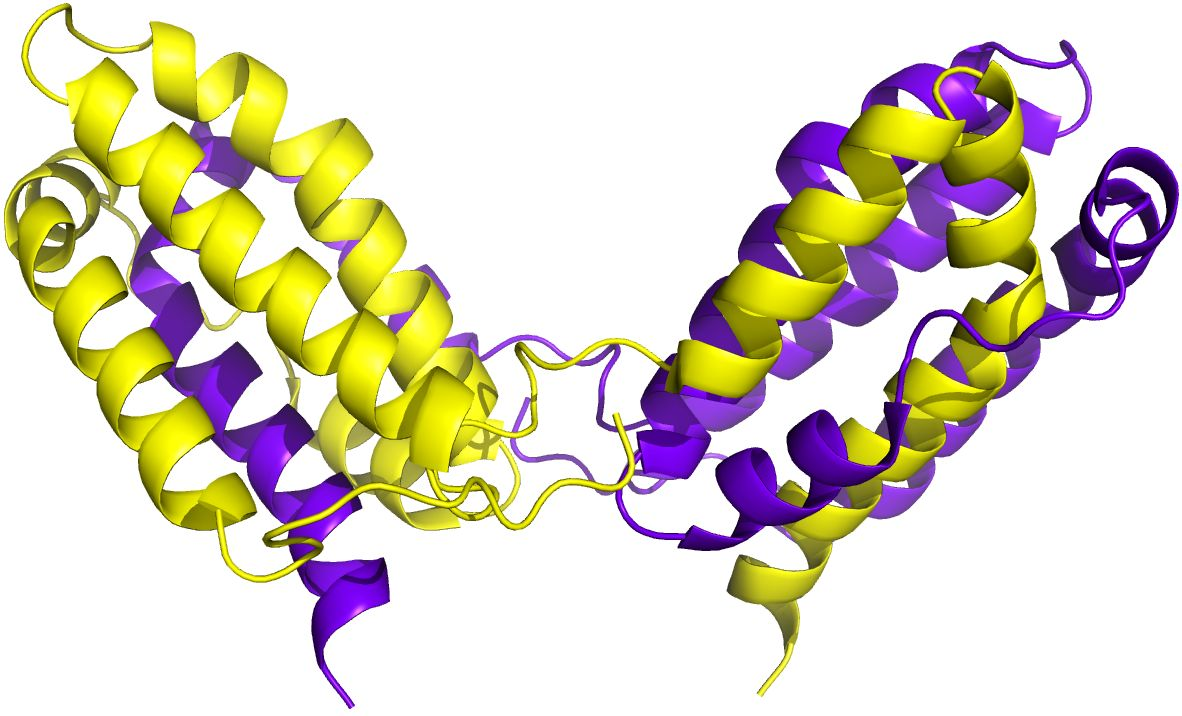
\includegraphics[width=1.0\textwidth]{gfx/background/IL10_2ilk_dimer_yellow_blue.jpg}
\caption[]{
2ILK hIL-10 dimer v shape}
\label{fig:bg:il10_dimer_vshape}
\end{figure}


Under physiological conditions in solution, IL-10 has been shown to
predominantly exist as a \textit{homodimer} --- the population of the monomeric
form is negligible \cite{syto_il10_homodimer_1998}. The crystal structure of the
IL-10 homodimer (according to PDB entry 2ILK) is visualized in
\cref{fig:bg:il10_dimer_vshape}. IL-10 is a so-called \enquote{intertwined} or
\enquote{intercalated} dimer of two sub-units (the IL-10 monomers), each
consisting of six helices, named A-F. The dimer has two domains, and each
monomer contributes four helices to one domain, and two helices to the other
domain. Helices A-D of one monomer together with helices E' and F' from the
other monomer form a distinctive six-helix domain --- for clarity, this is
color-encoded in \cref{fig:bg:il10_dimer_vshape}. The two monomers are
intertwined in a perfectly symmetric way, resulting in a \SI{180}{\degree}
(two-fold) rotational symmetry by which both domains of the IL-10 homodimer are
related.


 axis, by which


Explain stability of the structure, refer to disulfide bridges






\begin{figure}
\centering
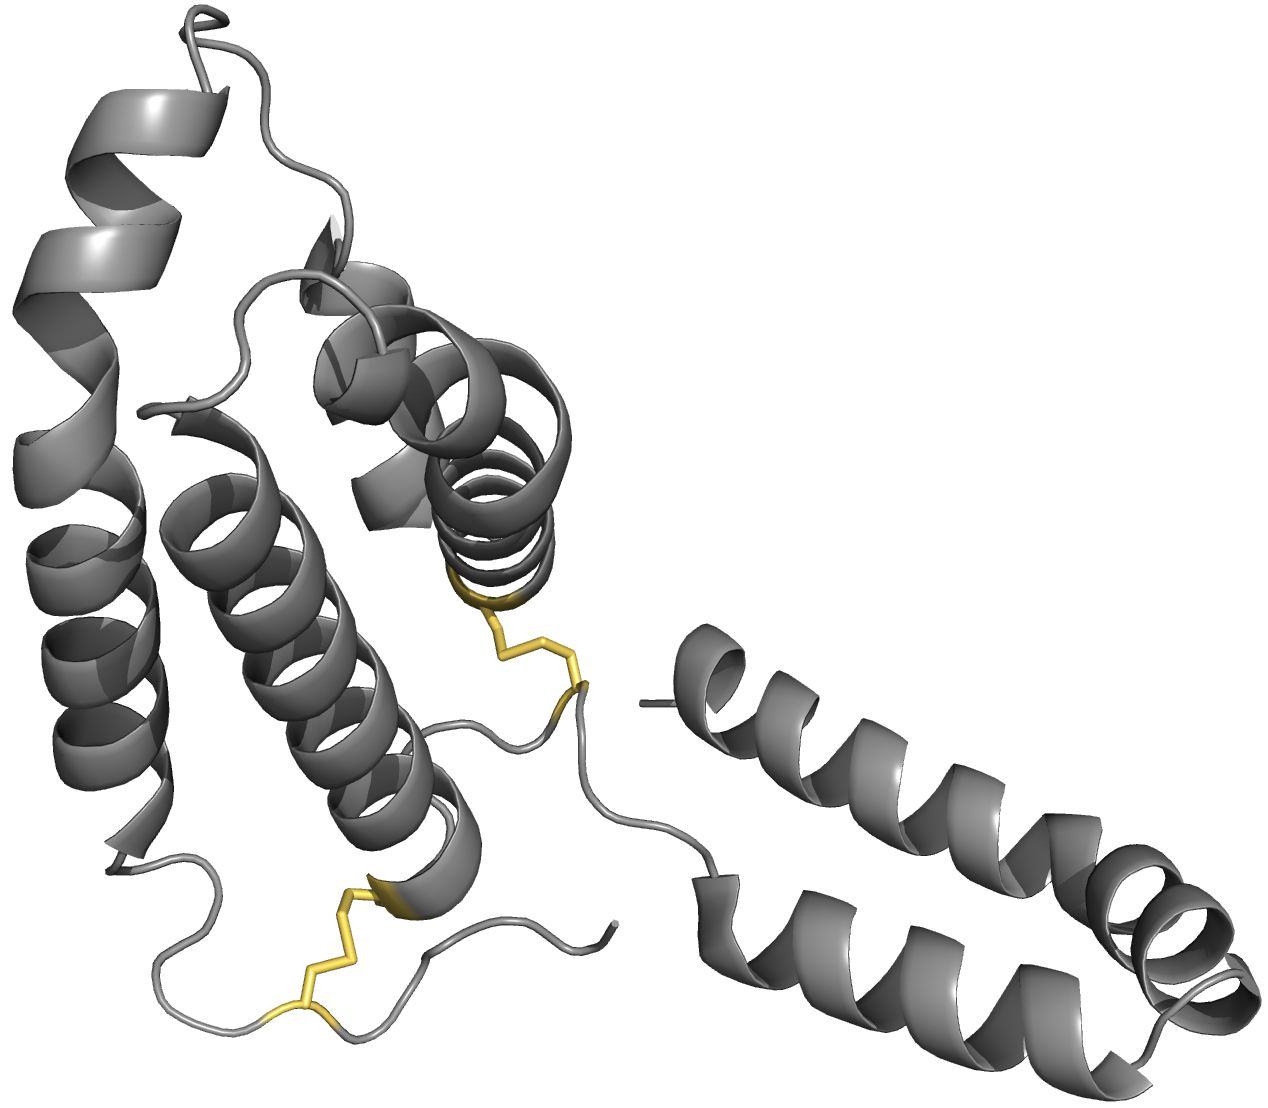
\includegraphics[width=1.0\textwidth]{gfx/background/IL10_2ilk_disulfide_with.jpg}
\caption[]{
2ILK hIL-10 monomer disulfide bridges stability
}
\label{fig:bg:il10_monomer_disulfide}
\end{figure}







    - Structure description
        exists mainly as homodimer [
            biochemistry, 1998, 37, 16943-16951, zdanov 1995]


    - IL-10 and its receptors
        - what is known in literature (current state of knowlege)
            R1+IL-10 structure
            R2 structure
            ternary complex binding models
            what is required for signaling? literature overview
        - a critical review: monomer
            minimal unit required for signaling (monomer)
        - IL-10 + R1 + R2 structure model from IL20 ternary complex

sequence, compare similarity and identity between hIL-10 and mIL-10.


\section{In-silico methods for investigating protein-GAG interaction}

%\subsubsection{GAG structures used in \textit{in silico} experiments}

\subsubsection{GAG representation approximations: isolation, length, purity}

As has been stated above, one of fundamental assumptions applied in this thesis
project: GAGs are treated as \textit{free} molecules.

%While it is likely
%that their tremendous length and also their covalent linkage to proteoglycans
%serve have an overall impact on the biological function of GAGs, it is a
%valid and well-established approximation to not account for these facts in
%molecular modeling studies that aim for resolving the molecular mechanism of
%protein-GAG interaction in atomic detail... in a biological function and overall  treated as

A more severe approximation applied in this thesis is the treatment of GAGs as
\textit{short} molecules. Considering the  mostly ranging from tetra- to hexasaccharides. Considering the level of atomic detail aimed for ... to be observed... in this
thesis project, GAGs are modeled as short molecules.


Also, when treating GAGs as short molecules, they are represented by the ideal
periodic repetition of the most frequently observed disaccharide unit,
impurities or variations in the monosaccharide sequence are ignored.

ir ideal periodic

explain DP, degree of polymerization

\nomenclature{dp}{degree of polymerization}

From Sergey: Computationally, GAG containing systems are still very challenging
to handle because of their high flexibility as it applies for saccharides in
general 15, importance of taking into account solvent mediated interactions16,17
and required proper treatment of electrostatics due to their charged nature
1,18,19. For heparin, in addition, the rings of IdoU2S can adopt two pucker
conformations (1C4 and 2S0) with comparable probability 20–23, which, therefore,
can represent a combinatorial task for modeling periodic molecules of heparin,
and which proper consideration is outside the scope of classical MD time scales
and common force fields at the moment 24,25. Nevertheless, both experimental and
computational studies show that even a single IdoU2S ring conformational change
significantly contributes to the specificity of GAG/protein complex formation
both structurally and thermodynamically 26,27. Moreover, it is known
that for relatively big systems like collagen-based matrixes, where interactions
with GAGs could be crucial for their mechanical properties 29–31, application of
the approaches which use only short GAGs does not seem to be proper.



\subsection{A primer on docking methods}


    - Methods applied in literature: a mini review
        AutoDock3 stands out, just by experience, not by concept
    - Problems of different complexity: local vs. global docking.
    - (AutoDock 3 protein-GAG blind docking validation study,
        Method, results, discussion, conclusion)

\lipsum[1-5]

\subsection{A primer on molecular dynamics simulations}

\lipsum[1-5]

\subsubsection{End-point free energy methods (\enquote{MM-PB(GB)SA})}
% This label is required in DMD chapter.
\label{methods:mmpbsa_mmgbsa}


Cite this: \cite{schlick_innovationsdynamics_2012} (volume 2, chapter 12).

\lipsum[1-5]




\section{Aim and scope of this thesis}

- Vision: gaining control over IL-10 function in artificial extracellular matrices

- Motivation and goal: investigate IL-10-GAG system with computational
      methods, in collaboration with...

The aim of this project is to unravel atomic details of IL-10-GAG interaction
with theoretical and computational means. If required, methodological approaches
are to be developed. Integration of \textit{in silico}-based predictions with
experimental results from collaborators will hopefully provide insights into the
mechanisms determining IL-10-GAG interaction. Methodology developed during this
project is applicable to protein-GAG systems in general, rendering it valuable
for a large field of research.



\hl{cite interleukin-2 -heparin interaction (mulloy, rider) !}

\lipsum[1-5]






%%\chapter{Structure and biology of the IL-10 system}
\chapter{Structure and biology of IL-10}


\section{A primer on IL-10 biology}

        in closing remarks, relate to extracellular matrix

\section{Description of IL-10 structure}

    - Structure description
        exists mainly as homodimer [
            biochemistry, 1998, 37, 16943-16951, zdanov 1995]

\section{IL-10 and its receptors}

    - IL-10 and its receptors
        - what is known in literature (current state of knowlege)
            R1+IL-10 structure
            R2 structure
            ternary complex binding models
            what is required for signaling? literature overview
        - a critical review: monomer
            minimal unit required for signaling (monomer)
        - IL-10 + R1 + R2 structure model from IL20 ternary complex


\lipsum[1-5]
%\chapter{In-silico methods for protein-GAG docking}
\lipsum[1-10]
\chapter{Protein-GAG binding site prediction via electrostatic potential analysis}

In this chapter we present a simple and yet efficient method for predicting
where on a protein a GAG would most likely bind, suggesting which amino acid
residues are likely to be involved in the interaction and which are not. The
method is based on numerical simulation of the electrostatic (i.e.\ Coulomb)
potential of the protein in water solution, and manual evaluation of the
topology of the Coulomb potential in space. Subsequently, we apply that method
to IL-10 and report our findings.

\section{Motivation}

Classical molecular docking approaches are used for creating binding predictions
for a given receptor-ligand system. Primarily, the correctness of a prediction
depends on the quality of the underlying physical or phenomenological model, and
whether the system under investigation is within the scope of validity of the
model. Since most molecular docking methods are trained for analyzing a limited
Cartesian volume in a \textit{local} search, application to larger search spaces
such as in \textit{global} docking dramatically lowers the confidence in the
resulting prediction. Therefore, common molecular docking methods should be
applied locally, and hence require \textit{a priori} knowledge about where on
the receptor the ligand most likely binds. The decision where to center the
local search on should be based on reliable data, otherwise the docking study
might be pointless. In the best case, knowledge about the binding site (the
region on the receptor that the ligand binds to) comes from experimental data,
e.g.\ from mutagenesis or NMR studies. However, in many cases no such
experimental data is available, as is unfortunately true for the IL-10-GAG
system. In such situations, it makes sense to consider \textit{in silico}
methods for binding site prediction.

With respect to protein-GAG systems, there is only few published work on this
topic. In \cite{hp_binding_sites_mulloy_2006}, Forster and Mulloy used AutoDock
version 2.4 \cite{autodock24} for globally docking rigid heparin molecules to
antithrombin and FGF2, and found that their docking procedure gave good
agreement with the corresponding crystal structures regarding the overall
position of the heparin binding sites. The authors state that the method may be
used as \enquote{hypothesis generation tool} rather than for providing
\enquote{details of interactions between specific atoms}. In another work
\cite{gandhi_bmp_heparin_binding_sites_2012}, the authors used PatchDock
\cite{patchdock_2002} for globally docking rigid heparin oligosaccharides to
BMP-2 and BMP-14 and state that \enquote{while there has been no validation of
the accuracy of the PatchDock scoring function for heparin interactions, these
docking results suggest the presence of two GAG binding sites in BMP-2}.

The above-cited studies do by no means provide a complete picture, but obviously
some of the established docking methods seem to be able to reflect certain
properties of protein-GAG systems. This is remarkable since none of these
docking methods has been specifically optimized for GAG ligands, let alone for
global docking, and strictly spoken, when applied to protein-GAG systems, these
docking methods are applied outside of their scope of validity. We postulate
that the reason for the surprising success in named studies is that protein-GAG
complexes are strongly driven by Coulomb interaction and that mentioned docking
methods incorporate Coulomb interaction with a significant weight in their
scoring functions.

In fact, heparin has the highest negative charge density among biological
macromolecules \cite{capila_linhardt_hep_prot_2002}. Standard literature on
protein-GAG systems such as
\cite{essentials_glycobiology_gags_2009,gandhi_structure_2008} stresses the
role of charge-charge interaction in protein-GAG systems in general. Many
publications focusing on individual protein-GAG systems identify charge
complementary as one of the driving mechanisms of the interaction between GAG
and protein
\cite{gandhi_bmp_heparin_binding_sites_2012,faham_heparin_1996,%
pichert_characterization_2012,rogers_gag_prot_prot_2011}.

We can conclude that the importance of Coulomb interaction is a distinctive
feature of protein-GAG systems. Notably, compared to other molecular interaction
types, the Coulomb interaction is a long range interaction and therefore
dominates all other contributions for larger distances. As of these
considerations, it seems to be reasonable to perform protein-GAG binding site
prediction purely based on the strength and topology (i.e.\ the
shape/distribution) of the electrostatic potential in the volume surrounding the
protein.

For a set of reference systems, we have investigated the relation between the
strength and topology of Coulomb potential and the actual experimentally
determined GAG binding site in order to determine whether the electrostatic
properties alone can assist in predicting a receptor GAG binding site. The
result of this study, be it positive or negative, in any case further enlightens
the role of Coulomb interaction in protein-GAG systems.


\section{Method}

\subsection{Coulomb potential simulation}

For a given protein, we calculated its electrostatic potential with a
finite-difference numerical solver applied to the linearized Poisson-Boltzmann
(PB) equation. The PB equation is widely used for implementing a class of
implicit solvent models to describe solvent-mediated electrostatic interactions.
These models have been demonstrated to be reliable in reproducing the energetics
when compared with explicit solvent molecular dynamics simulations and
experimental measurements for a wide range of systems \cite{honig_estatic_1995}.
In the PB model we have applied, the solute (protein) is described by an
atomic-detail representation, while the solvent molecules are treated as a
continuum. The solute is modeled as a dielectric body whose shape is defined by
atomic coordinates and atomic radii. A set of point charges at the atomic
centers produces an electrostatic field in the solute region as well in the
solvent regions. The overall electrostatic field is the sum of the Coulombic
field of the solute and the corresponding solvent reaction field (since it is
heavily polarizable).

We calculated the overall electrostatic potential of the protein in water using
the PBSA program shipped with AmberTools 13 \cite{case_amber_12} with default
parameters. The protein point charges were parameterized according to the FF99SB
force field \cite{case_amber_12}. The grid spacing was set to \SI{1}{\angstrom}.



$1\,\angstrom$.
Isosurface visualization of the potential was done in VMD





(choosing the modified ICCG solver
applied to the linearized Poisson-Boltzmann equation).
\cite{vmd1996}.


\subsection{Coulomb potential evaluation}

\section{Application to reference systems}


\begin{figure}
\centering
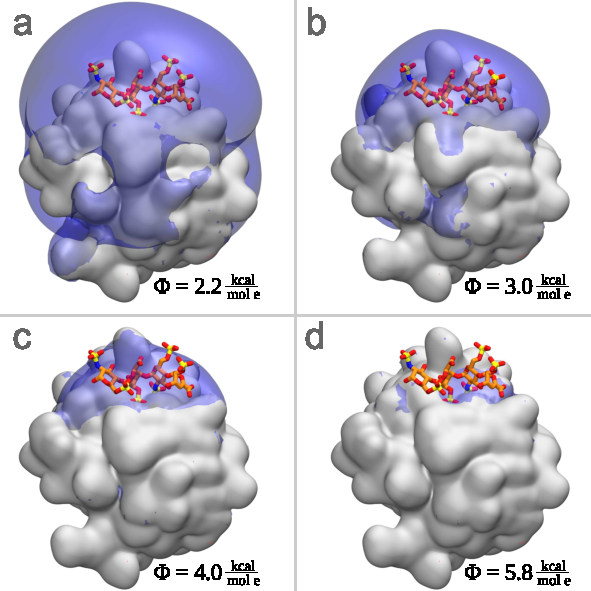
\includegraphics[width=0.9\textwidth]{gfx/bspred/fgf2_coulomb_isosurfaces_different_values_03_ds.pdf}
\caption[]{
Isosurface representation of FGF2's Coulomb potential (blue), shown for multiple
isovalues isovalues $\Phi$. The molecular surface of FGF2 is shown in gray, its
heparin ligand pose as determined experimentally is shown as sticks with C atoms
in orange (structure taken from PDB ID 1BFB). }
\label{fig:bspred:fgf2_multi_iso}
\end{figure}



\subsection{Results and discussion}

TODO: argue, why application of complex docking methods only allowed us to
speculate why they are sometimes succcessfull (see motivation part), but now,
in a controlled environment with a very simple model (only coulomb), we can
directly conclude that coulomb interaction IS the dominating interaction that
alone determines binding site for many systems.


Discuss FGF2, SDF1, and CD44!

Refer to \hl{The result of this study, be it positive or negative, in any case
further enlightens the role of Coulomb interaction in protein-GAG systems.}

\section{Application to IL-10}

\begin{figure}
\centering
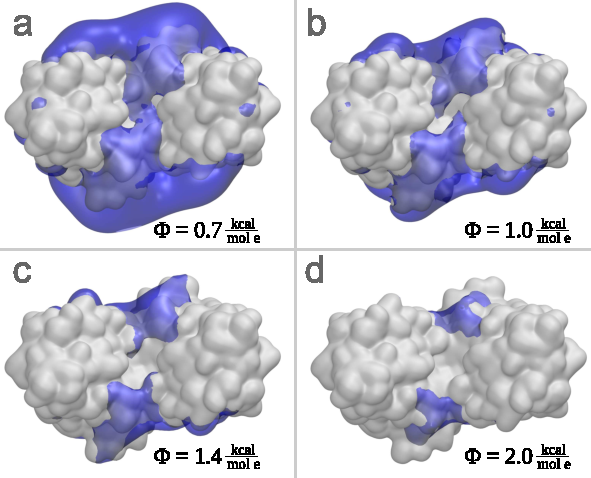
\includegraphics[width=1.0\textwidth]{gfx/bspred/il10_top_coulomb_isosurfaces_different_values_03_ds.pdf}
\caption[]{
Isosurface representation of IL-10's Coulomb potential (blue), shown for
multiple isovalues isovalues $\Phi$. The molecular surface of the IL-10 dimer is
shown in gray (structure taken from PDB ID 2ILK).
}
\label{fig:bspred:il10_multi_iso}
\end{figure}


\begin{figure}
\centering
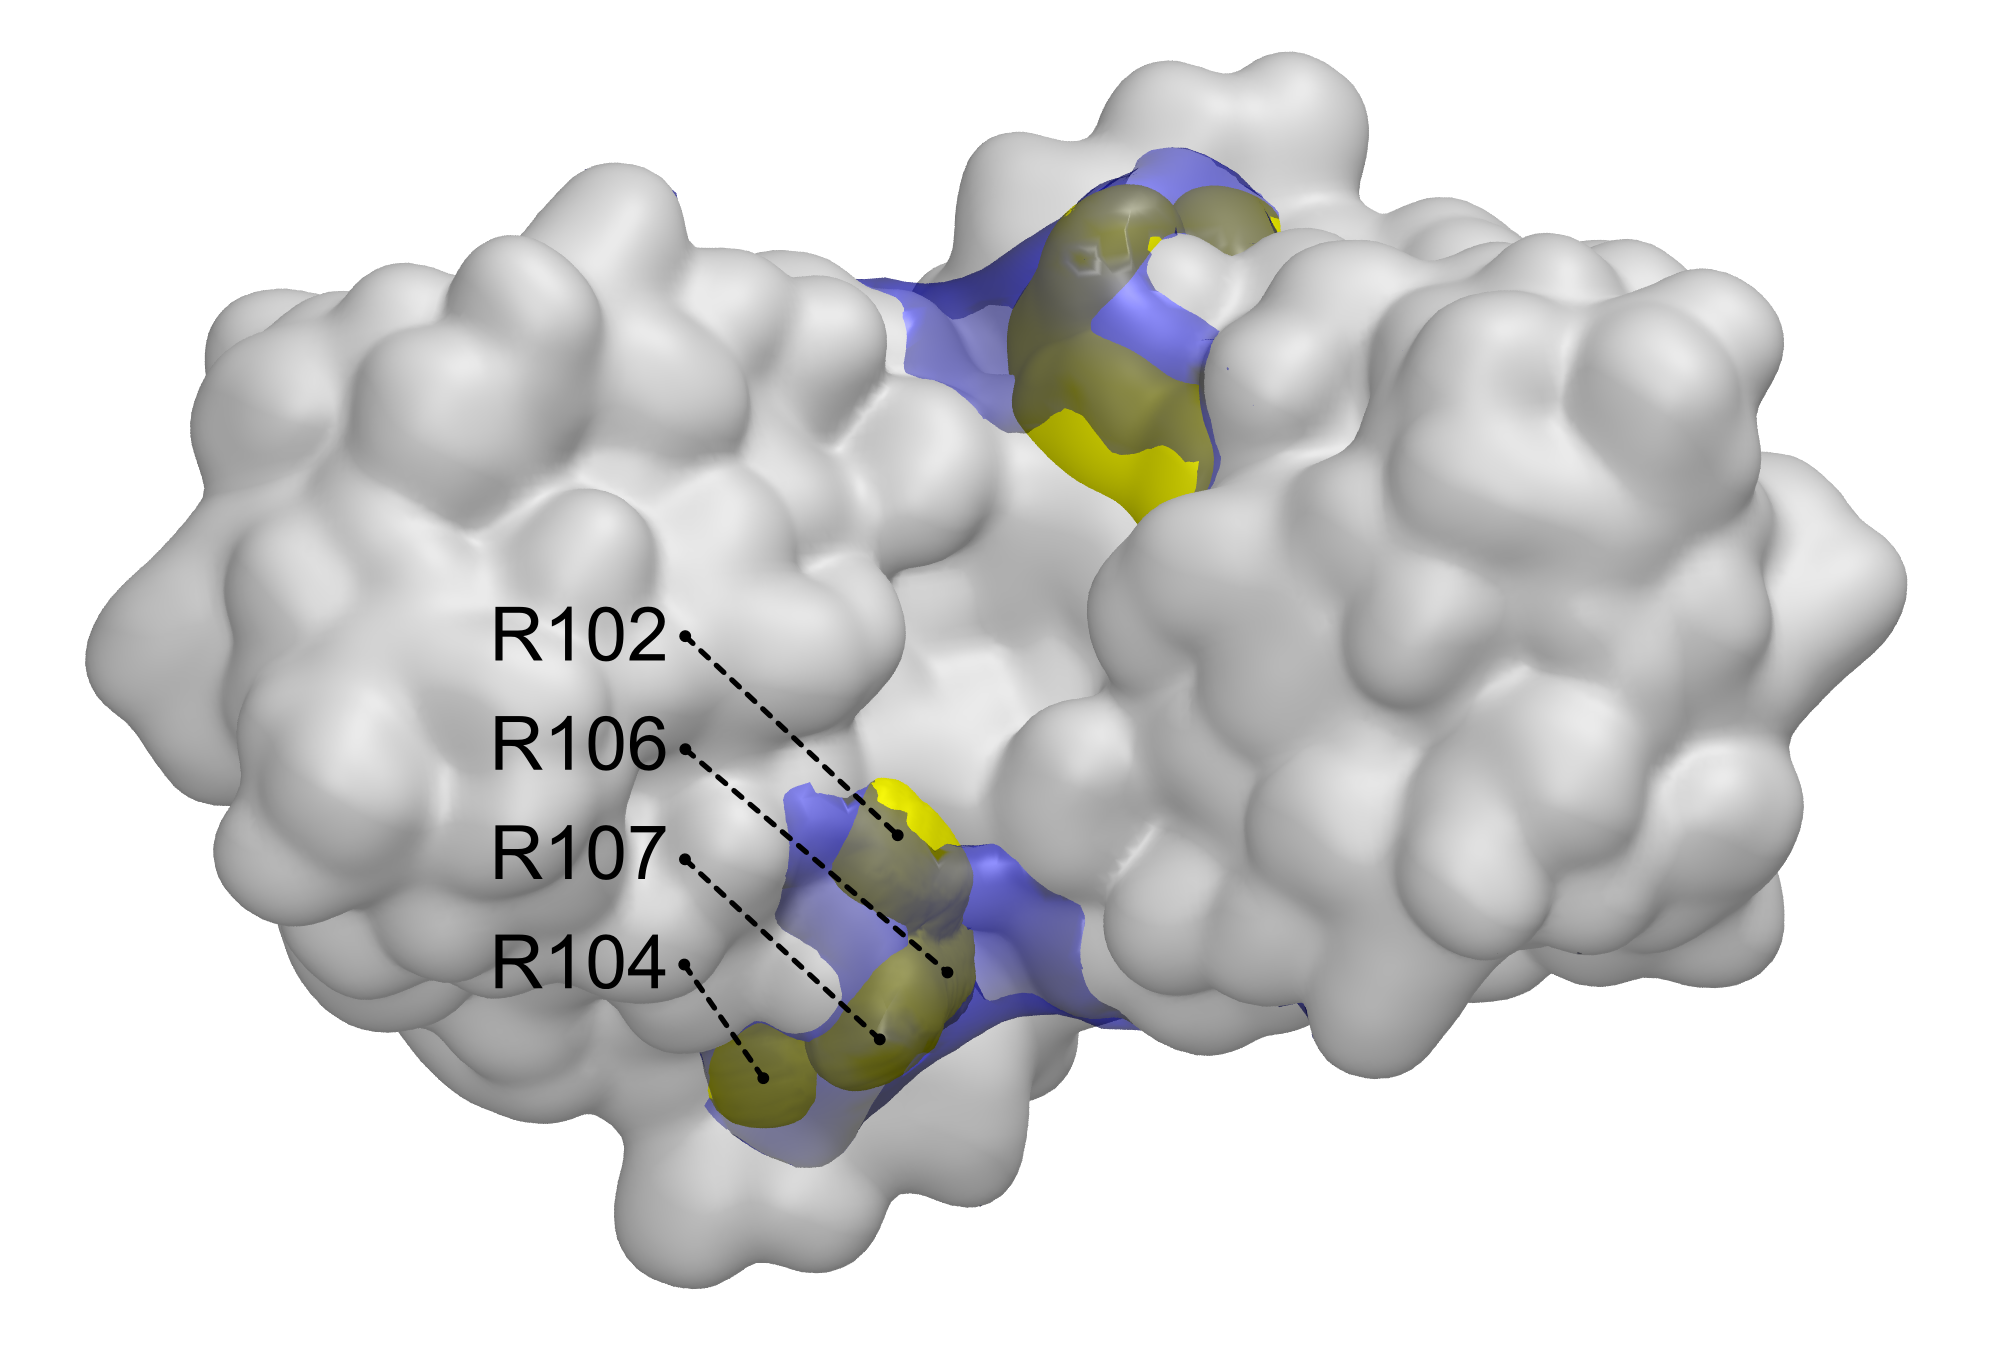
\includegraphics[width=0.9\textwidth]{gfx/bspred/SI_figure_IL-10_coulomb_isosurface_1_9kcalmol.png}
\caption[]{
Isosurface representation of IL-10's Coulomb potential with the isovalue $\Phi =
\SI{1.9}{\kilo\calory\per\mole\per\elementarycharge}$ (blue). The molecular
surface of the IL-10 dimer is shown in gray, the molecular surface of arginines
102, 104, 106, 107 is shown in yellow (structure taken from PDB ID 2ILK). This
representation allows to see where the Coulomb potential (for a given isovalue)
protrudes into space further than the molecular surface, and has been shown to
provide useful evidence about where GAGs bind to a protein \hl{(REF)}. Hence,
IL-10-GAG interaction most likely takes place within the two symmetrically
arranged regions indicated here.
}
\label{fig:bspred:il10_estatic_pred}
\end{figure}


\subsubsection{Electrostatic potential analysis in protein-GAG systems}

\hl{Generalize this section, keep details for DMD chapter. At the moment most of
this is simply copied from the DMD manuscript.}

The electrostatic potential often dominates protein-GAG interaction
\cite{gandhi_structure_2008}. In this section, we discuss the electrostatic
properties of the receptors in the TDS with the goal to determine how these
properties could assist defining a receptor target region for DMD and also to be
able to relate docking performance to electrostatic characteristics of the
receptor.


Poisson-Boltzmann-based numeric calculations of the electrostatic potential of
molecules are most error-prone near the dielectric boundary, i.e.\ on the
molecular surface. We therefore did not simply map the potential on the
molecular surface but analyzed the topology of the potential with an isosurface
representation while varying the isosurface value. This allows for an
understanding  of the distribution of the potential in space and how strongly it
would affect a ligand. \cref{fig:bspred:sdf1_estatic} shows an isosurface of the
Coulomb potential of SDF-1. \cref{fig:bspred:various_estatic} shows analogous
isosurface representations of the electrostatic potential for the other TDS
complexes. For this type of visualization, the isovalue selection was done
individually for each receptor in the TDS such that only a small part of the
isosurface is protruding into space further than the molecular surface of the
receptor.



\begin{figure}
\centering
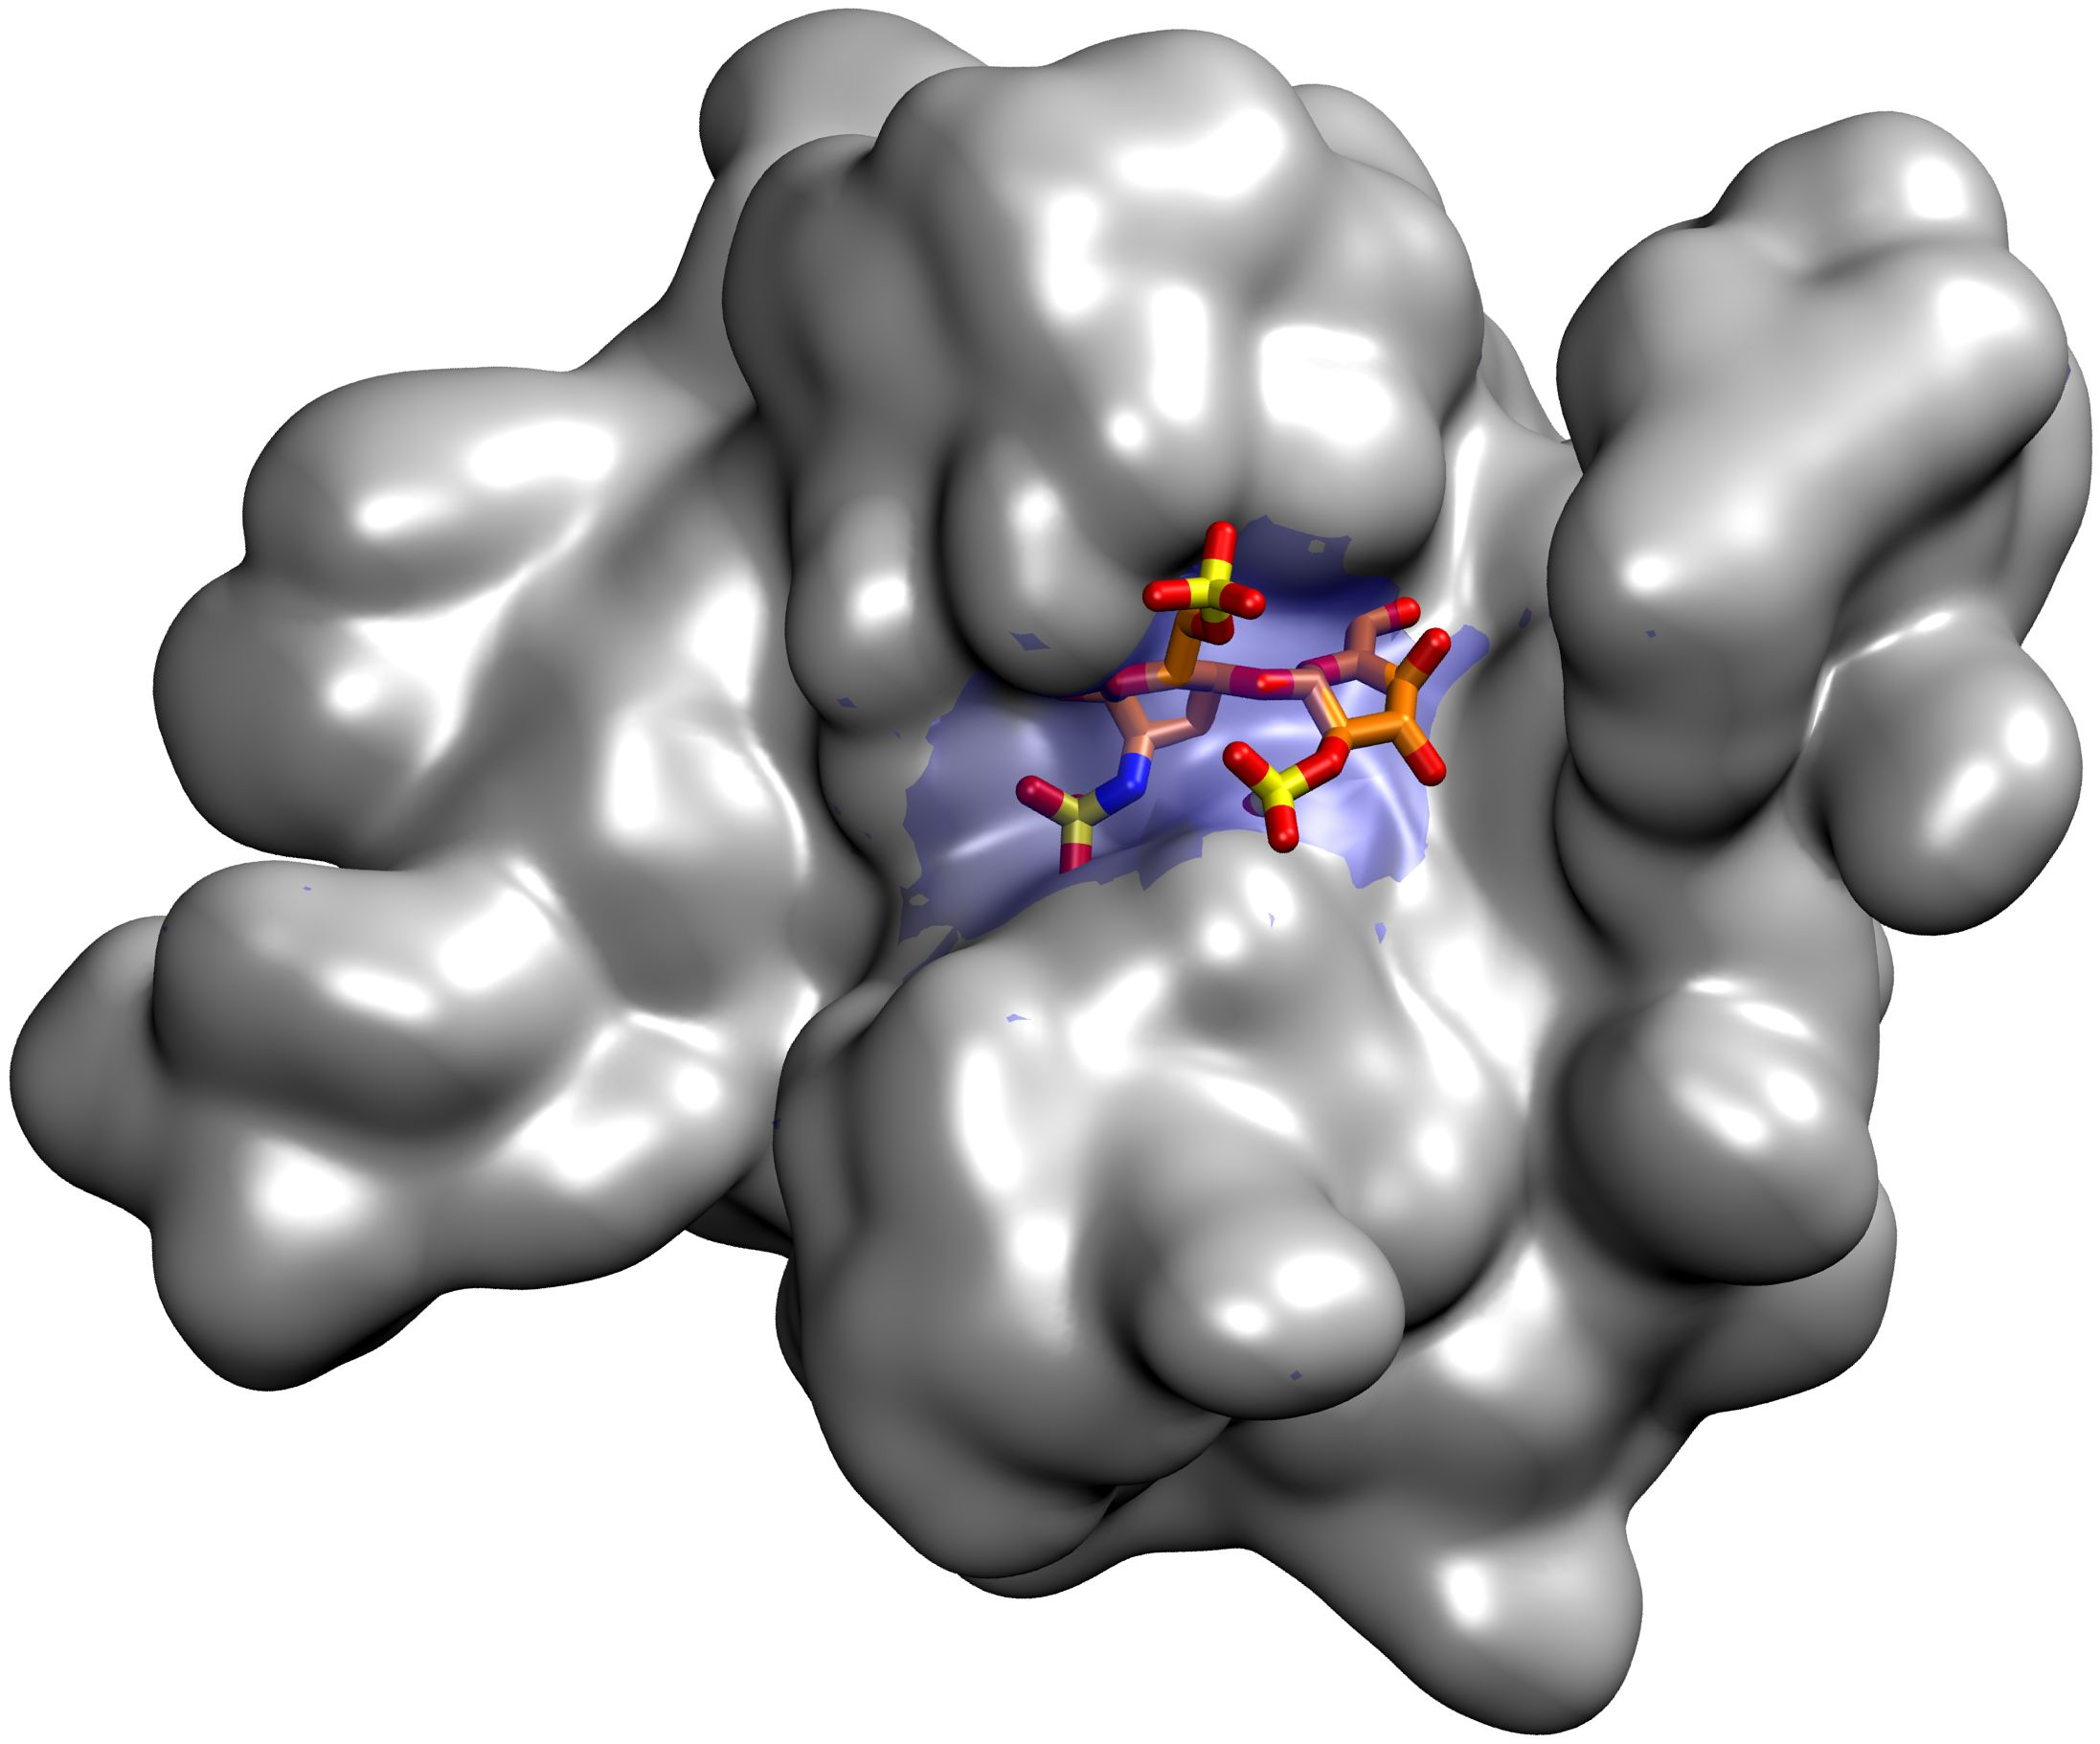
\includegraphics[width=0.9\textwidth]{gfx/bspred/sdf1_isopot_8_5_view1_rotated_jcc_pub_001.jpg}
\caption[]{
Isosurface representation of SDF-1's electrostatic potential with the isovalue
$\Phi = 8.5\,\mathrm{kcal\,mol^{-1}\,e^{-1}}$ (blue). The molecular surface of
the SDF-1 dimer is shown in grey, the heparin ligand as determined
experimentally (PDB ID 2NWG) is shown as sticks with C atoms in orange.
}
\label{fig:bspred:sdf1_estatic}
\end{figure}

Regarding the SDF-1-HP complex, our electrostatic potential evaluation procedure
unambiguously identifies the GAG binding site as determined experimentally. With
$8.5\,\mathrm{kcal\,mol^{-1}\,e^{-1}}$, the isovalue chosen is the largest among
the TDS complexes, indicating that SDF-1 has the strongest electrostatic
attraction to its ligand. In case of FGF2-HP (\cref{fig:bspred:various_estatic}), the
binding site is also unambiguously defined by the electrostatic potential. For
CD44-HA, the net electrostatic interaction between both molecules is slightly
repulsive. There is no obvious relation between the electrostatic properties of
the receptor and the binding site location. CathK and CathKmut exhibit
electrostatic attraction for negatively charged molecules in the experimentally
observed ligand binding site as well as in an adjacent region. We observe that
electrostatic potential analysis provides a clear idea whether GAG-binding to a
given receptor is mainly driven by Coulomb interaction. If a protein is known to
bind GAGs, and the electrostatic potential topology is as unambiguous as in case
of SDF-1 or FGF2, a GAG binding site prediction based on the presented procedure
is reliable. Visualization of the electrostatic potential can also be helpful to
\textit{a priori} exclude regions of the receptor surface when repulsive to
negatively charged ligands. Furthermore, this analysis shows that knowledge
about the electrostatic potential distribution in space can be used to choose a
reasonable ligand \enquote{entry lane} orientation for the tMD pulling process.


\begin{figure}
\centering
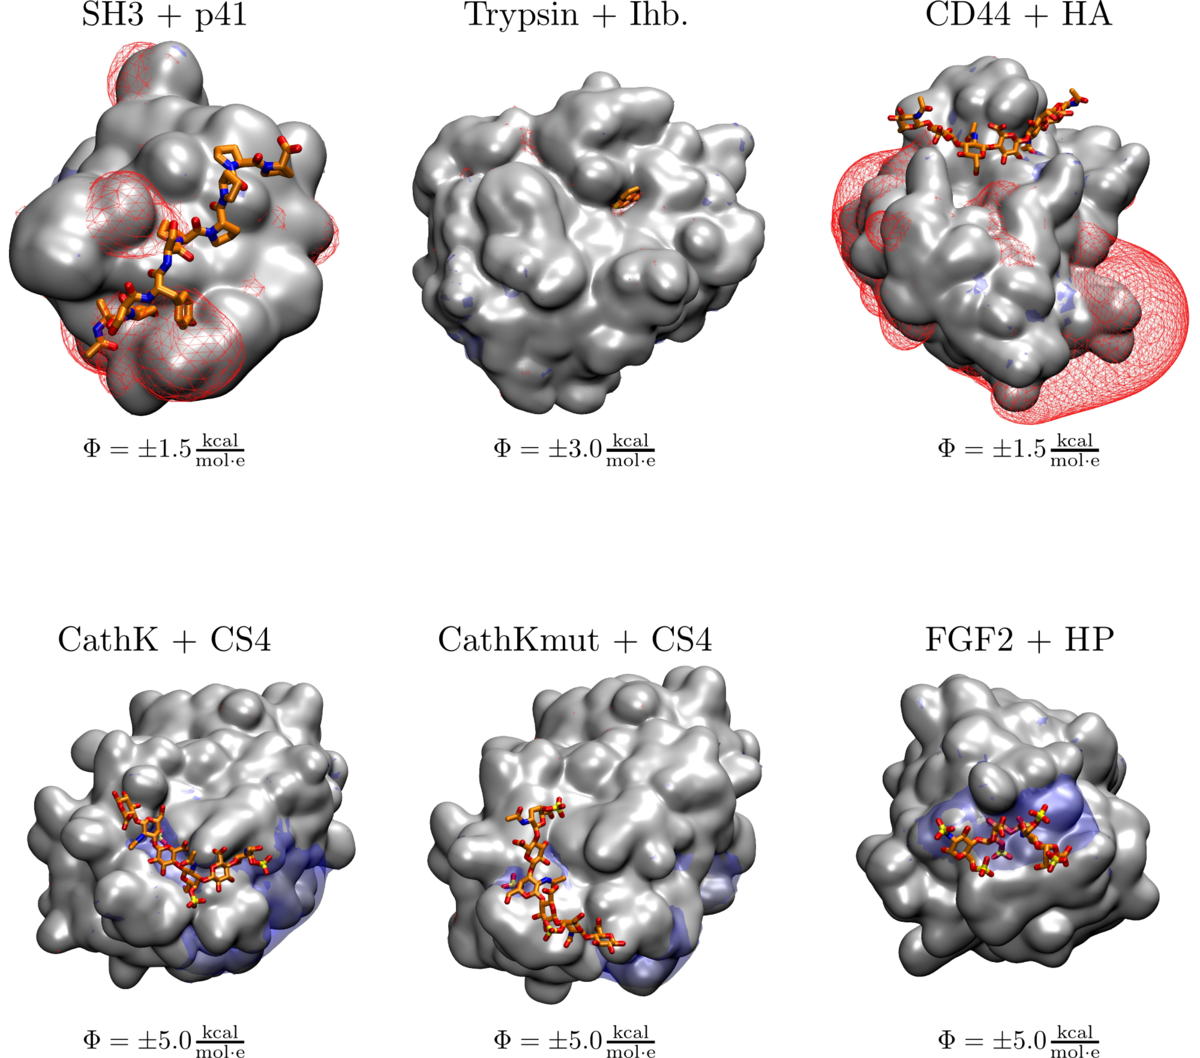
\includegraphics[width=0.9\textwidth]{gfx/bspred/suppl_figure_estatic_distributions_004_1200.png}
\caption[]{
Visualization of the electrostatic potential of the receptors from the TDS
(molecular surfaces in gray) with their ligands as experimentally determined
(shown as sticks with C atoms in orange). Blue/red: Isosurface representation of
the receptor's electrostatic potential with isovalue Ф (attractive/repulsive for
negatively charged molecules, respectively).
}
\label{fig:bspred:various_estatic}
\end{figure}


\hl{Create more convincing Figure than bspred:variousestatic.
Include more interesting complexes, remove uninteresting ones.}

The SH3-p41 complex is dominated by non-polar interactions, rendering the
Coulomb potential analysis inconclusive. Recognition of the Trypsin inhibitor in
its  binding pocket is affected by polar interactions. The electrostatic
potential, however, does not display clear characteristics to predict a binding
region.



\hl{INCORPORATE:} The method surely is more useful than the popular method of
heparin binding site consensus sequence search (cardin, weintraub) (hileman,
linhardt), which has already been applied to interleukin-10 before. Its about
structure, not sequence, that is also why Forster and Mulloy state that
\enquote{though some 'consensus sequences' for heparin binding have been
identified, they are neither necessary nor sufficient to define a heparin
binding site} \cite{hp_binding_sites_mulloy_2006}.

\chapter{Interpreting docking results: docking solution ensemble clustering}

In this chapter we describe why the conduction of a meaningful docking study
requires proper creation and analysis of an ensemble of docking solutions and
explain why clustering is an essential step for making reasonable predictions
about where and how a ligand binds to its receptor. This topic is unfortunately
not well discussed in current molecular docking literature, and existing
technical implementations for the clustering of docking solutions often do not
fit the scientific question and therefore may produce misleading results. Here,
we present a method optimized for clustering docking solution ensembles of GAG
molecules.

\section{Relevance of docking solution clustering}
In the framework of this thesis the term \enquote{docking solution} shall be
understood as a set of ligand atom coordinates, i.e. the spatial arrangement of
ligand atoms in the reference coordinate system as defined by the receptor
molecule. As a result of the statistical nature of the docking problem and the
use of pseudo random numbers in implementations of common docking search
algorithms, independent runs of the same docking method are expected to produce
different docking solutions. That is why a molecular docking method should be
applied repetitively, resulting in an ensemble of docking solutions.

The spatial distribution of docking solutions in that ensemble is governed by a
certain previously unknown probability distribution, which itself is implicitly
determined by the molecular interaction model and search algorithm implemented
in the docking method. Given that we trust the molecular interaction model, the
ultimate goal of a docking study is to obtain the global maximum (and/or some
local maxima) of the named probability distribution. Concept-wise, this is
equivalent to searching the state with highest probability, i.e. lowest energy.
Obtaining local maxima requires complete sampling of that unknown probability
distribution. That is why a docking method must be repeated until convergence
in the spatial distribution of the docking solutions is achieved. Only then the
ensemble reproduces the previously unknown probability distribution and reflects
the molecular interaction model as implemented by the docking method.

If convergence is observed, the next step is to identify the local maxima in the
spatial probability distribution of docking solutions. This problem can be
reformulated in terms of density, i.e. as finding the densest agglomerations of
docking solutions in the ensemble. However, a simple evaluation of the
distribution of atoms or molecules per volume would not provide useful results,
because a ligand molecule is comprised of multiple different atoms and has
various asymmetries with respect to shape and property. Spoken freely, the task
is to find agglomerations of docking solutions that are highly \textit{similar}
to each other. Hence, a promising approach is to evaluate the density in terms
of the \textit{similarity} between any two given docking solutions in the
ensemble, subject to the condition that a meaningful molecular similarity
measure can be found. In an abstract sense, the task is to identify groups of
highly similar docking solutions and separate them from the bulk. This task fits
the general description of \textit{data clustering} as found in
\cite{tan_data_mining}:

\begin{adjustwidth}{1cm}{1cm}
\textit{
The goal is that the objects within a group be similar to one another and
different from the objects in other groups. The greater the similarity (or
homogeneity) within a group and the greater the difference between groups, the
better or more distinct the clustering.
}
\end{adjustwidth}

Any data clustering method has only two major ingredients:
\begin{itemize}
\item the \textit{distance metric}, quantifying the similarity between any two
given objects.
\item a \textit{clustering algorithm}, classifying the objects into groups,
based on their mutual similarity.
\end{itemize}

In conclusion, the most probable ligand molecule placement as predicted by a
certain docking method can be found by clustering the (converged) ensemble of
docking solutions, using a meaningful distance metric and a clustering algorithm
that fits the problem. It is important to appreciate that both ingredients must
be adjusted to the scientific question, otherwise the result of docking solution
clustering might be meaningless and/or incomparable to other docking studies.
Within the next sections, we introduce a distance metric optimized for GAG
molecules and describe a clustering algorithm appropriate for clustering
molecular structure ensembles in general.


\section{A meaningful distance metric for GAG molecules}
RMSatd


\section{Algorithm of choice: DBSCAN}

\subsection{Clustering method overview}

    - Clustering methods overview
        hierarchical clustering implemented in AutoDockTools
            badly implemented, due to $N^2$ dependence very long runtimes
        other methods, quick
        DBSCAN, explain why it makes sense for molecular structures
        cite cpptraj, which also started implementing it

\subsection{DBSCAN parameter optimization}

    - change criteria from eps/minp to N clusters / members
    - reproducibility!
    - comparability among studies
    - characterization of a cluster via eps


\section{Clustering method implementation}

\subsection{Efficient implementation of DBSCAN for numpy}

        - Custom implementation of the DBSCAN algorithm

\subsection{Efficient implementation of RMSatd for numpy}

        - Custom implementation of the DBSCAN algorithm
        - examples
            http://scikit-learn.org/stable/modules/clustering.html
            http://bit.ly/1pKNv7v


\subsection{Parameter optimization}

        - brute force plus local optimization

\subsection{Architecture of cluster-pdb-structures}

            command line tool, simple PDB parser files
            distance matrix calculation on multiple cores via Unix fork()

            input: structure ensemble, DBSCANopt parameters
            output: structure files, stat summary


            open source at bitbucket..



\chapter{Dynamic Molecular Docking}

This chapter is a customized version of \cite{dmd_samsonov_gehrcke_2014}, where
we have published the description and validation of Dynamic Molecular Docking.

% American Chemical Society’s Policy on Theses and Dissertations
% http://pubs.acs.org/userimages/ContentEditor/1218205107465/dissertation.pdf

\section{Abstract}
We present Dynamic Molecular Docking (DMD), a novel
targeted molecular dy\-namics-based protocol developed to address ligand and
receptor flexibility as well as the inclusion of explicit solvent in local
molecular docking. A class of ligands for which docking performance especially
benefits from overcoming these challenges are glycosaminoglycans (GAGs). GAGs
are periodic, highly flexible and negatively charged polysaccharides playing an
important role in the extracellular matrix via interaction with proteins such as
growth factors and chemokines. The goal of our work has been to develop a proof
of concept for an MD-based docking approach and to analyze its applicability for
protein-GAG systems. DMD exploits the electrostatics-driven attraction of a
ligand to its receptor, treats both as entirely flexible and considers solvent
explicitly. We show that DMD has high predictive significance for systems
dominated by electrostatic attraction and demonstrate its capability to reliably
identify the receptor residues contributing most to binding.

\section{Rational}

Molecular docking has been extensively applied for drug
discovery in the recent decades \cite{klebe_recent_2000,
cheng_structure-based_2012}. Whereas molecular docking methodologies demonstrate
to be very successful and continue to develop rapidly, they still suffer from a
number of limitations \cite{moreira_proteinprotein_2010,
andrusier_principles_2008,lensink_docking_2010}. What holds true for practically
all docking methods is that the reproduction of an experimentally observed
docking pose is less challenging than proper scoring of this pose by energy
\cite{kim_assessment_2008, plewczynski_can_2011,smith_csar_2011}. In the
majority of docking approaches, only small ligands can be treated as entirely
flexible in order to limit the size of the conformational search space. Although
flexible treatment of the ligand is crucial for obtaining meaningful results,
ligand flexibility often can only be approximated, especially in protein-protein
docking \cite{ritchie_recent_2008}. Another severe approximation applied in most
docking methods is static treatment of the receptor even though protein side
chain flexibility is crucial for ligand binding, and substantial conformational
changes can occur in the receptor structure induced by interaction with a ligand
\cite{gunasekaran_how_2007,gutteridge_conformational_2005}. Finally, most of the
established docking approaches do not explicitly account for solvent molecules,
whereas many studies point out their importance in docking calculations
\cite{van_dijk_solvated_2006,baron_water_2010,roberts_ligandprotein_2008,
thilagavathi_ligand-protein_2010}.

A particularly challenging class of ligands for which docking
performance is especially limited by the above-mentioned issues are
glycosaminoglycans (GAGs), which are periodic negatively charged linear
polysaccharides mainly located in the extracellular matrix. Through interaction
with their protein targets they participate in a number of key processes
involved in cell regeneration and proliferation, angiogenesis, metastasis and
lipid metabolism \cite{hynes_extracellular_2009, macri_growth_2007,
barbero_chembiochem_2013}. Due to the occurrence of numerous sulfate and
carboxyl groups, GAGs have a high charge density, rendering long-range Coulomb
interaction to be crucial for binding to proteins
\cite{mulloy_specificity_2005}. The significance of electrostatic interaction
underlines the importance of taking explicit solvent molecules as binding
mediators into account when GAGs are used as ligands in molecular docking
\cite{samsonov_docking_2011}. Moreover, the orientation and conformation of long
side chains of charged protein residues may be greatly influenced by interaction
with a GAG ligand. In consequence, flexible treatment of the receptor during
GAG-docking is of special relevance. In addition, a similar spatial distribution
of functional groups in GAGs independent of the reducing/non-reducing end
orientation \cite{hp_binding_sites_mulloy_2006} as well as their high
flexibility \cite{bitomsky_docking_1999} substantially contribute to the
challenges in protein-GAG docking. Overall, the prediction of protein-GAG
complexes via molecular docking comprises a good example of some of the current
limitations in the field of classical molecular docking.

Classical docking approaches are generally optimized for having relatively
modest computational requirements and therefore enable the quick investigation
of single complexes as well as the execution of large-scale studies involving a
large number of different complexes. Taking into account ligand and receptor
flexibility as well as treating solvent explicitly clearly increases the
computational complexity of docking approaches. However, in view of the
ever-increasing computing power, a new generation of docking methods should
evolve, which though being computationally more demanding, aims to deal with the
above-mentioned challenges.

Molecular dynamics (MD) techniques are established for rigorous studies of
intermolecular interactions \cite{karplus_molecular_2005}. Beyond that, MD
methods have already been used in docking approaches for overcoming the
challenges of both ligand and receptor flexibility
\cite{chaudhuri_application_2012, antes_dynadock_2010}. Furthermore, standard MD
methods allow for the inclusion of explicit solvent via well-established water
models. The application of MD techniques is limited by high computational cost,
which previously has hindered their usage in high-throughput approaches for drug
discovery. However, nowadays, advanced computational resources are available and
specialized hardware (such as graphics processing units, GPUs) can be used to
dramatically increase the performance of MD simulations, making the
establishment of MD in the field of docking gradually feasible.

We propose Dynamic Molecular Docking (DMD), a combination of established
MD-based methods specifically designed for tackling the above-mentioned
challenges in protein-GAG docking. DMD is a targeted MD-based approach where the
ligand, which is initially placed at a distance from the receptor so that their
interaction is negligible, is slowly pulled towards a receptor target region by
applying a time-dependent distance restraint. During this process, both receptor
and ligand are treated as entirely flexible in explicit solvent. The time-
dependent distance restraint applied in DMD is usually used in steered molecular
dynamics simulations, which are performed for studying the energetics of
processes that generally happen on timescales too large for being treated by
classical MD simulations \cite{xiong_free_2006}, such as protein folding, ligand
unbinding and large-scale conformational alteration. In DMD, once the ligand
reaches the receptor, the distance restraint is switched off and a long free MD
simulation is carried out, allowing for the mutual adjustment of receptor
residues and GAG as well as for extensive GAG-internal degree of freedom
sampling. The obtained trajectory data are then used for \textit{i)} extracting
a docking solution (the coordinates of the ligand relative to the receptor) and
\textit{ii)} for the characterization of this docking solution. In terms of
molecular docking, this method keeps binding pose search well as binding pose
scoring consistent, in the sense that both use the same potential as given by
the MD force field and the parameterization of the molecular system.

Classical molecular docking is usually based on a phenomenological model,
whereas the internal parameters have been trained based on a set of molecular
reference systems (often, machine learning tools are applied for this task).
This raises the question about the applicability of such model to systems
outside the training data set, and about the validity of the resulting data. In
contrast, one of the main conceptual advantages of molecular dynamics
simulations compared to classical docking approaches is that the underlying
model and its parameters are (classical) physics-based. The parameters have been
developed over years with the goal to make dynamics simulations reproduce the
classical chemical and physical properties of the simulated system. Hence, if
properly set up, MD simulations produce data that is generally more trustable
and resilient than data produced by machine learning-based docking methods.

One of the main concepts of a DMD study is that pulling process and subsequent
free MD are repeated \textit{many} times in independent simulations. This allows
for the creation and evaluation of an ensemble of docking solutions rather than
the interpretation of single trajectories. In this ensemble, the energetically
more favorable states are the more likely ones. Subsequent spatial clustering of
this docking solution ensemble identifies those docking solutions that appeared
with highest probability and, therefore, lowest energy. We should note that a
meaningful DMD study requires a reasonable assumption about the binding region
it is focused on. However, there is no general dependence of the DMD protocol on
the confidence in the binding region assumption --- selection of the binding
region and local docking are independent tasks.

\begin{figure}
\centering
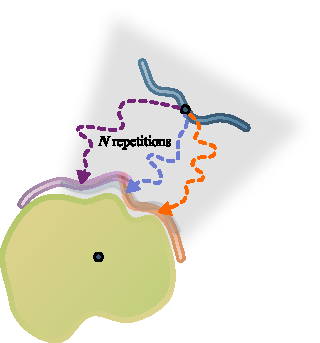
\includegraphics[height=8cm]{gfx/dmd/scheme_n_repetitions_for_thesis_002.pdf}
\caption[]{Schematic representation of the DMD pulling process. Starting from a
distal position, the ligand (blue) is pulled towards its receptor (green).
During this process, the ligand moves along a random path. The pulling process
is repeated $N$ times in independent simulations. Most of the resulting ligand
trajectories lie within a certain \enquote{entry lane}, as depicted here in grey
shade. Each pulling process yields an individual final ligand state (purple,
blue, orange) near the receptor surface.}
\label{fig:dmd:n_repetitions}
\end{figure}


\section{General method description}
\subsection{Data production}

A DMD study for a given receptor-ligand complex implies performing $N$ (e.g.
100) independent DMD runs. The number of independent repetitions $N$ must be
large enough for obtaining convergence regarding certain ensemble properties.
Each DMD run starts with a randomly oriented ligand molecule placed at a
distance from the receptor (ligand re-oriented model, LROM). The first step of a
DMD run is a targeted molecular dynamics (tMD) simulation in which the ligand is
pulled towards a pre-defined target region on the receptor via a time-dependent
decrease of the distance $d(t)$ between one central atom in the ligand and one
core atom in the protein receptor. Among DMD run repetitions, most of the ligand
trajectories lie within a certain \enquote{entry lane} which is focused on a
point near the receptor surface, the focus point $\bm{F}$, and therefore
defining the target region (\cref{fig:dmd:n_repetitions}). All final tMD states
have the central ligand atom positioned on the surface of a sphere defined by
the protein core atom (the center of the sphere) and the final distance $D$ of
the tMD pulling process (the radius of the sphere). Based on the final state of
each tMD simulation, the second step of a DMD run relaxes the system via a free
MD simulation. Geometrical definitions, system preparation, and details about
tMD and free MD parameterization as well as subsequent trajectory data analysis
methods are provided in the following sections.

\begin{figure}
\centering
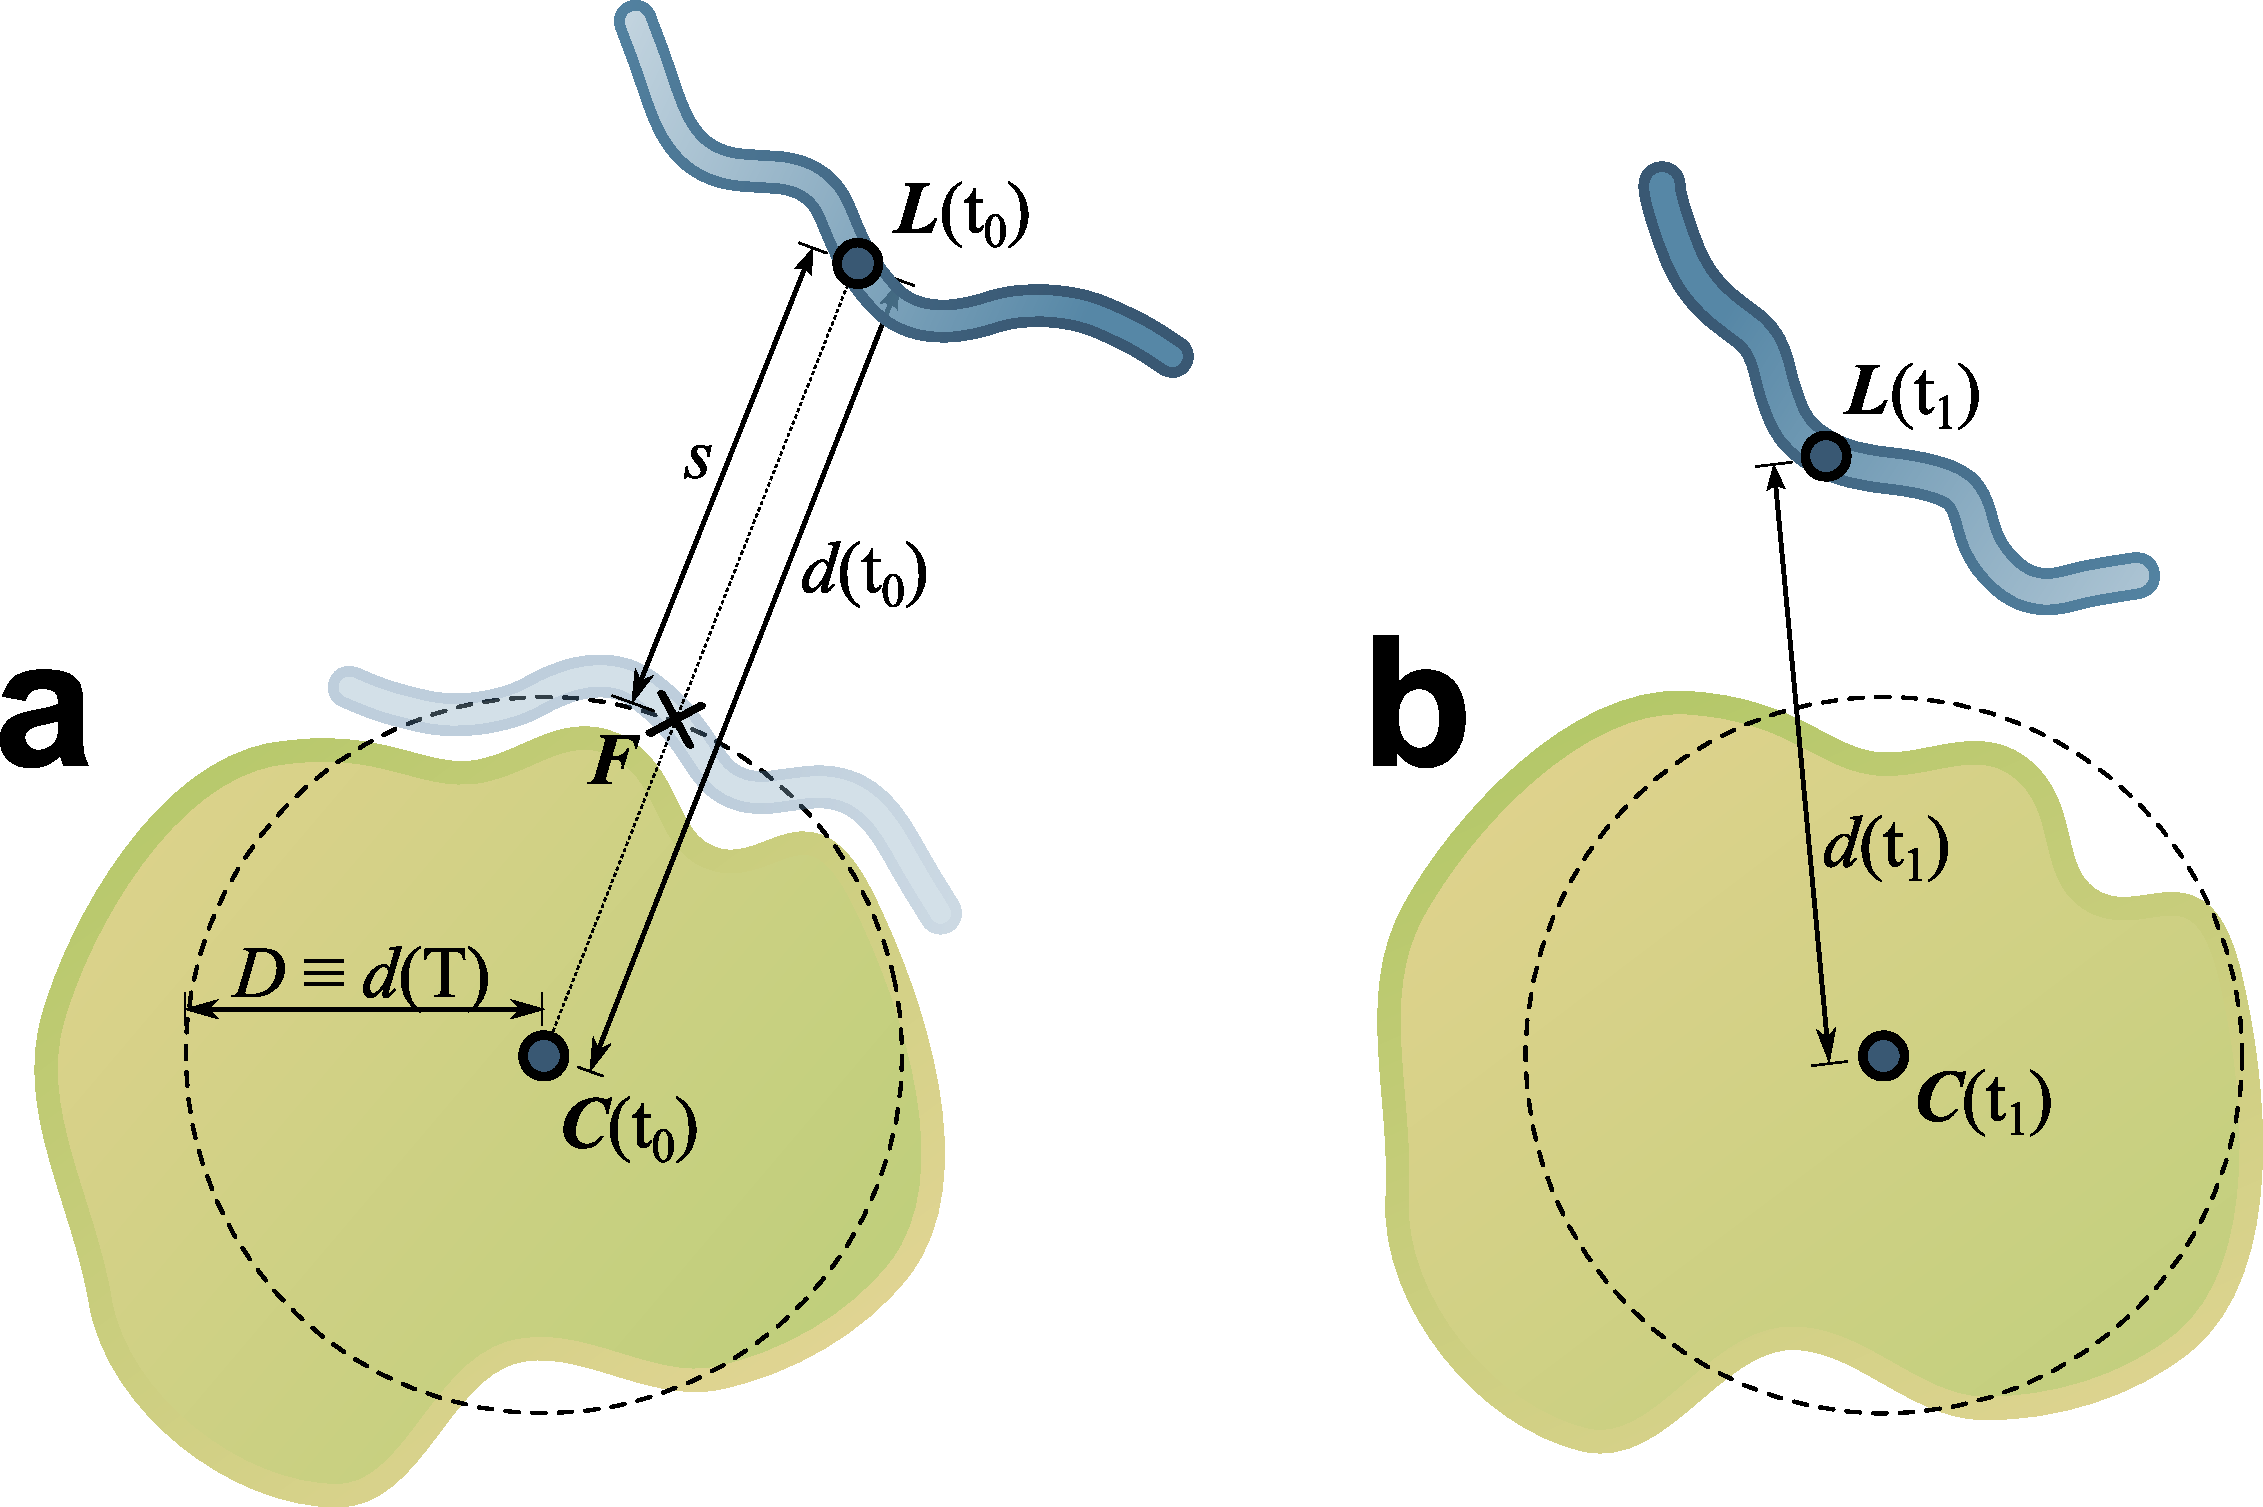
\includegraphics[height=7cm]{gfx/dmd/scheme_geometry_two_panels_002.pdf}
\caption[]{
\textbf{a}: System configuration at time $t_0$ right before the pulling process,
referred to as the ligand-reoriented model (LROM, with the displaced ligand in
dark blue). The central atom of the experimentally determined ligand position
(light blue) has been placed to a distal position $\bm{L}(t_0)$ along the axis
given by a receptor core atom at point $\bm{C}(t_0)$ and the focus point
$\bm{F}$. $s$ is the displacement length. The ligand has been randomly rotated
around its central atom. The distance between $\bm{C}(t_0)$ and $\bm{F}$ defines
the final distance $D$ for the ligand pulling process. The initial distance
$d(t_0)$ between $\bm{C}$ and $\bm{L}$ is $D+s$.
\textbf{b}: arbitrary state within the pulling process, during which the
distance $d(t)$ between central ligand atom at point $\bm{L}(t)$ and protein
core atom at point $\bm{C}(t)$ is decreased over time $t$. Right after the
pulling process, all final ligand states have their central atom placed on the
sphere that is indicated here with a dashed line.
}
\label{fig:dmd:geometry_scheme}
\end{figure}

\subsubsection{Preparation of ligand-reoriented models (LROMs)}
An LROM contains
the receptor as well as the ligand placed in a distal, re-oriented position. Per
TDS complex, ten LROMs have been created, differing only in ligand orientation
around its central atom. For a given complex, LROM creation requires the
selection of a \textit{central ligand atom}, definition of a \textit{focus
point} $\bm{F}$ near the surface of the receptor within the anticipated binding
region, definition of a \textit{ligand displacement length} $s$ and selection of
a \textit{core atom} at point $\bm{C}$ within the receptor. The distance between
focus point and core atom defines the final distance $D$ of the tMD pulling
process, i.e.\  $d(T) \equiv D \equiv  \lVert \bm{F}-\bm{C} \rVert$. Initially,
at time $t_0$, the ligand is placed distal from the receptor with its central
atom lying on the axis defined by $\bm{F}-\bm{C}$
(\cref{fig:dmd:geometry_scheme}a). The starting coordinate for the central
ligand atom is defined as

\begin{equation}
\bm{L}(t_0) = \bm{F} + s \frac{\bm{F}-\bm{C}}{D}.
\end{equation}

For each TDS complex, multiple LROMs should be prepared as follows. First, the
structure of the biological unit of the protein receptor is to be taken from the
corresponding experimental data source (3D structure from crystallography or
NMR). The coordinates of a central atom in the ligand as found in the
experimentally determined structure are to be used as focus point. The core atom
in the receptor must be selected fulfilling three criteria: \textit{i)} it is a
backbone atom within a helix or beta sheet in the protein core, \textit{ii)} the
line connecting core atom and $\bm{F}$ (defining the orientation of the ``entry
lane'' is roughly perpendicular to the surface comprising the anticipated
binding region, and \textit{iii)} the surface of the sphere around the core atom
with radius $D$ has significant overlap with the molecular receptor surface in
the receptor target region. Distal ligand placement is to be followed by
multiple random ligand rotations uniformly distributed in 3D space with
$\bm{L}(t_0)$ being the rotation center. Each rotational ligand corresponds to
one LROM.

\subsection{Data analysis}

MD simulations provide a plethora of data extraction and analysis possibilities,
and in general the researcher is not limited in his/her creativity to extract
interesting quantities from the raw data of a DMD study. Namely, the available
raw data are the trajectories of $N$ tMD and $N$ free MD simulations, which in
total usually comprise one or more microsecond(s) of simulated real time. In
this section, we provide an overview about how DMD data analysis should be
performed in general, classify the different approaches, and discuss some
obvious data extraction techniques.

\begin{figure}
\centering
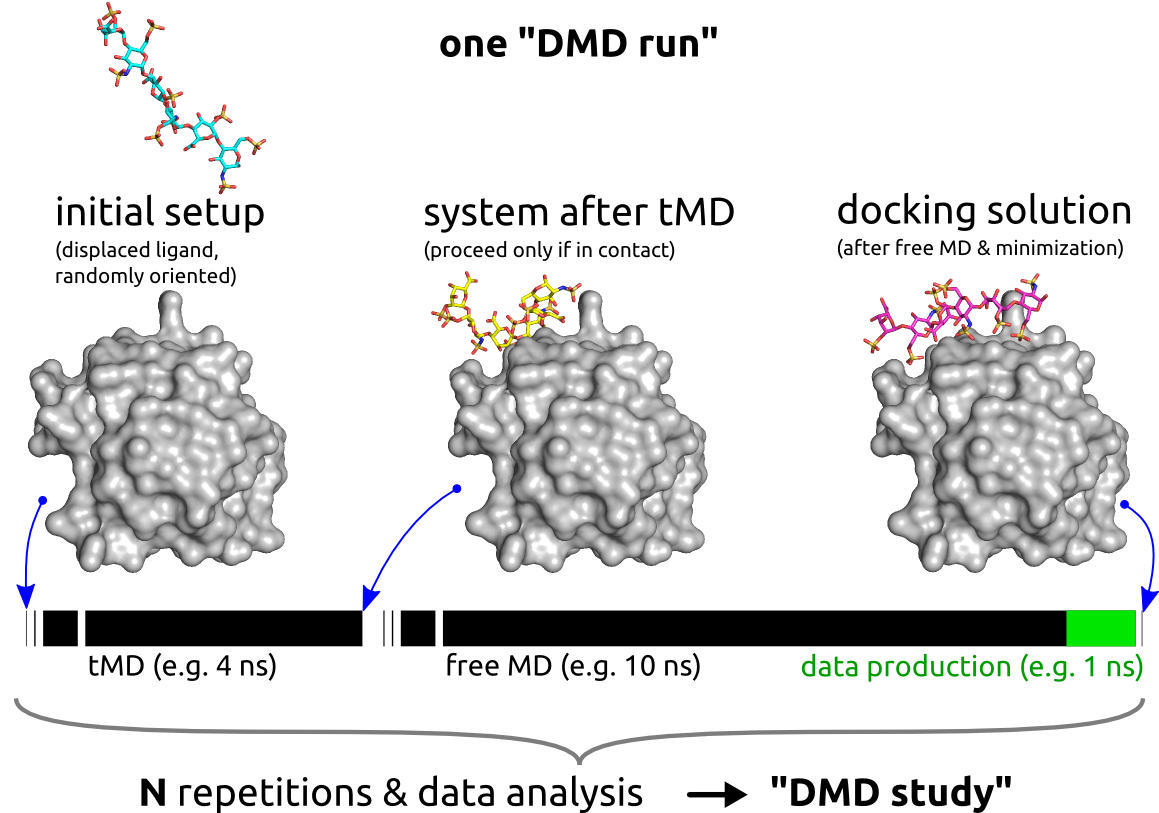
\includegraphics[width=1.0\textwidth]{gfx/dmd/dmd_timeline_for_thesis_09.png}
\caption[]{
Schematic overview of the chronological sequence of a DMD run, and definition of
the term \enquote{DMD study}. The black bars, read from left to right, provide
an overview of the time course of a single DMD run: its starts off with the
initial system (example system shown at the left, with the protein surface in
gray and the ligand shown in blue sticks) and proceeds with the targeted
molecular dynamics (tMD) process. The final tMD system state (central example
system with the ligand shown in yellow sticks) is further processed in a free MD
simulation. tMD and free MD involve the usual MD preparations (minimization,
heat-up, and equilibration), as indicated by the shorter black bars. The
coordinates of a single docking solution are the result of energy minimization
of the final free MD state (example system on the right, with the ligand shown
in magenta sticks). Extraction of data for docking solution characterization is
limited to the final fragment of free MD, as indicated in green.}
\label{fig:dmd:timeline}
\end{figure}


First of all, we need to clarify which fractions of the trajectories of a DMD
study are interesting for data extraction. Method characterization for sure
requires analysis of all trajectory data created. Application of the method,
however, focuses on docking solution \textit{generation} and
\textit{characterization}. For this task, it is required to ignore most parts of
the trajectory data, namely the entire tMD process as well as the first major
part of the free MD simulations. These parts are strongly relevant for sampling,
they however are not applicable for characterizing the final state of a DMD run,
i.e.\ the \textit{docking solution} corresponding to that run. That is why we
have (arbitrarily) decided to use the last \SI{1}{\nano\second} of the free MD
simulation, for extracting data about a single docking solution. For
clarification, \cref{fig:dmd:timeline} shows the relation of a \enquote{DMD
study} and single \enquote{DMD runs}, as well as a time line of a single DMD run
with specific labeling of the time interval relevant for data extraction.

\subsubsection{Characterization of single docking solutions}

Conceptually, data extraction is performed for single DMD runs. That is,
evaluation of the tail of any given free MD simulation yields certain
quantities, and these quantities correspond to one DMD run only. Such quantities
can be used for characterizing the single docking solution as obtained from that
DMD run. These quantities can be classified as either of \textit{static}, or of
\textit{dynamic} nature. Static quantities are derived from the energy-minimized
free MD final system state, i.e.\ from \textit{one} set of coordinates only.
Meaningful examples of such static quantities are:

\begin{itemize}
\item The minimal distance between receptor and ligand, i.e.\ the distance
between those two atoms in receptor and ligand which are closest to each other
of all receptor-ligand atom pairs. This quantity describes whether receptor and
ligand are in contact or not. An atomic contact in an organic system usually
leads to an inter-atomic distance of slightly below \SI{2}{\angstrom}.
\item The average minimal distance between receptor and ligand, i.e.\ find the
closest atom in the receptor for each atom in the ligand and build the mean of
all resulting atom pair distances. For ligand molecules such as GAGs this
quantity describes the alignment of receptor and ligand: a small value suggests
that the ligand is entirely aligned with the receptor. A large value on the
other hand means that most parts of the ligand are not in contact with the
receptor.
\end{itemize}

These quantities can be convenient for automatically filtering DMD runs, e.g.\
for separating out those docking solutions where receptor and ligand are not in
contact with each other, by pure geometric criteria. Dynamic quantities on the
other hand implicate analysis of multiple MD trajectory frames. That is, they
are based on multiple sets of coordinates that represent the \textit{dynamic}
nature of the system as simulated by the MD method. Meaningful examples of such
dynamic quantities are:


\begin{itemize}
\item The internal ligand flexibility, measured in \si{\angstrom}. Can be
calculated by iterating through the MD frames while aligning the ligand
coordinates of the current frame to those in the first frame, and then building
the root mean square distance ($RMSd$) for all MD frames in question,
yielding a time series of $RMSd$ values. The standard deviation of this time
series represents the fluctuation of the data, i.e.\ the internal ligand
flexibility.

\item The mobility of the ligand relative to the receptor, measured in
\si{\angstrom}. The procedure is the same as described before, with the
difference that the receptor is aligned to the receptor prior to measuring the
$RMSd$, i.e.\ the receptor defines the reference coordinate system, and not the
ligand. Hence, the standard deviation of this $RMSd$ time series represents the
overall mobility of the ligand with respect to the receptor.

\item The average number of hydrogen bonds established between ligand and
receptor. For simple analyses, it is safe and established to infer hydrogen
bonds by simple atom type, distance, and angle criteria
\cite{hbonds_crystal_survey,hbonds_sulfur_1991}, as implemented in the MD
trajectory analysis software cpptraj \cite{cpptraj_2013}. The average number of
hydrogen bonds throughout the tail of the free MD trajectory gives quite useful
clues about how many high affinity atomic contacts are established in the
binding mode described by the docking solution. The and the corresponding
standard deviation of this time series expresses the stability of the hydrogen
bonding network.

\item Hydrogen bonds can also be analyzed by tracking the existence of specific
acceptor-donor atom pairs over time, which allows for determination of the time
fraction of occupancy of such a specific pair. Acceptor-donor atom pairs can
then be ranked by their relative occupancy, in order to determine the importance
of single hydrogen bonds.

\item Hydrogen bonding can also be analyzed by tracking the occupancy of single
donors or acceptors over time, yielding the importance of single atoms in the
ligand or atoms/amino acid residues in the protein receptor.

\item Estimation of the free energy of binding via end-point free energy methods
such as MM-PBSA or MM-GBSA (cf.\ \cref{methods:mmpbsa_mmgbsa}). These methods
are usually applied to a time series of MD trajectory frames, and yield an
estimate for the contributions of different interaction types to the overall
binding affinity, including standard deviation and standard error of the mean.
Different docking solutions of the same molecular system can be ranked by such
free energy of binding estimates, providing a meaningful and convenient tool for
comparison among different docking solutions.

\item So-called single-residue energy decomposition (SRED) can be performed via
a specialized form of the MM-GBSA analysis (cf.\ \cref{methods:mmpbsa_mmgbsa}).
SRED assigns an energy value for each amino acid residue in the protein receptor
and therefore enables meaningful ranking of such residues by importance for
ligand binding.
\end{itemize}


\subsubsection{Merge the data: extraction of ensemble properties}

We have stressed before that an essential concept of DMD is the creation and
analysis of an entire \textit{ensemble} of docking solutions. In fact, the
characterization of single docking solutions does not necessarily yield
trustable or even meaningful insights about the protein-ligand system under
investigation. The ensemble properties, however, are assumed to be
\textit{converged}, i.e.\ an independent repetition of the same DMD study would
yield different individual docking solutions, but ensemble properties of the
same kind. As of the validity of the underlying model, a converged result of MD
simulations is usually \textit{reliable} and \textit{meaningful}. Therefore, we
seek to extract ensemble properties of a DMD study. \textit{Static}
coordinate-based docking solution ensemble evaluation by means of clustering has
been discussed before in \cref{chapter:clustering}. Here, we describe an
additional approach for extracting \textit{dynamic} DMD study ensemble
properties that are likely to provide essential insights about the molecular
system under investigation.

Two of the single docking solution analysis types listed above are qualified for
\textit{merging} their results among (nearly) \textit{all} docking solutions:
hydrogen bonding occupancy analysis and single-residue energy decomposition. The
idea behind such data merge operation is to find those residues in the protein
receptor that are most important for ligand binding, whereas the entire DMD
study provides the corresponding data, rendering the outcome significant and
trustable. Essentially, the merge operation is comprised of \textit{filtering}
useful docking solutions, and \textit{averaging} their corresponding quantities
for single residues in the protein receptor. The filtering step makes sure that
no invalid (e.g.\ unbound) docking solutions contribute to the final result. The
averaging operation merges the ensemble data, enriched with statistics: it
usually makes sense to track standard deviation and standard error of the mean
in order to decide whether the merge provides valid data or not. The result of
the merge is an \textit{ensemble-derived quantity} for each protein residue.
Obviously, the average of a certain quantity measured for a \textit{diverse} set
of docking solutions does not provide a meaningful absolute value. The merge
operation, however, provides a meaningful \textit{ranking} among the different
protein residues. Simply spoken, this kind of analysis helps identifying those
residues that are most important for binding in most of the single DMD runs ---
just in a systematic and reliable way.


\section{DMD implementation for this thesis project}

\subsection{Molecular dynamics protocol}

The DMD-related molecular dynamics simulations performed in the context of this
PhD project were set up, performed, and analyzed using Amber 12 and AmberTools
12 \cite{case_amber_11}. The FF99SB force field was used for parameterization of
the peptidic parts in the investigated complexes. GAG force field parameters
were created based on GLYCAM 06 version g \cite{kirschner_glycam06:_2008} and
sulfate partial charges obtained by RESP fitting calculations at the level of
6-31(d)G for methylsulfate. All systems were solvated in a box of TIP3P water
with a minimum of \SI{8}{\angstrom} distance between solute and box boundaries.
The systems were neutralized by adding Na$^{+}$ or Cl$^{-}$ counterions. The MD
time integration step was set to \SI{2}{\femto\second}, whereas bonds including
hydrogen atoms were length-constrained by the standard SHAKE method. During MD,
non-bonded interactions were switched off for atom pairs further apart than
\SI{8}{\angstrom}. The Particle Mesh Ewald method was used for treating
long-range electrostatic interactions.

Each simulated system went through minimization, heat-up, equilibration, and
production steps. During the first stage of minimization, only the solvent was
relaxed. During the second stage, the entire system was minimized without
restraints. System heat-up to \SI{300}{\kelvin} was performed within
\SI{20}{\pico\second} of simulated real time in the canonical ensemble (NVT)
using the Langevin thermostate and periodic boundary conditions. Subsequently,
\SI{500}{\pico\second} of MD in the isothermal-isobaric ensemble (NPT) with
Langevin thermostate and Berendsen barostat under periodic boundary conditions
were carried out for system density equilibration. The following production
stage of duration $T$ was performed in the NVT ensemble with the Berendsen
thermostat and periodic boundary conditions.

%For complexes involving heparin, weak torsional restraints were
%applied in order to keep the pyranose rings of IdoA(2S) in the $^{1}C_4$
%conformation. This conformation has been shown to be one of the two
%predominantly populated ones{\cite{almond_jacs_2010}} and was observed
%experimentally in the structure of the FGF2-HP complex in our test data set (PDB
%ID 1BFB). The applied restraints enable to define and control the specific
%%conformation of each IdoA(2S) ring throughout the entire DMD study, since its
%natural ring conformer population is not properly reproduced by GLYCAM
%06{\cite{gandhi_idoa2s_2010}}.

\subsubsection{Targeted and free molecular dynamics.}
The LROMs were prepared for MD and time-evolved following the general MD
protocol as described above. During the tMD production stage, core atom and
ligand center atom were exposed to an additional time-dependent harmonic
potential

\begin{equation}
U(t) = \frac{1}{2} k \left( d(t)-d(t_0) + vt   \right)^2
\end{equation}

with force constant $k=200\,\mathrm{kcal\,mol^{-1}\,A^{-2}}$, pulling velocity
$ v = s/T$ and

\begin{equation}
d(t) = \lVert \bm{L}(t)-\bm{C}(t) \rVert.
\end{equation}

This potential enforces the distance between the selected ligand center atom and
the protein core atom to linearly decrease with time $t$ in the interval from
$D+s$ to $D$ (\cref{fig:dmd:geometry_scheme}b). For all tMD simulations, we used
a pulling velocity of $s=\SI{30}{\angstrom}$ per $T=\SI{4}{\nano\second}$.

For each DMD study, we prepared ten LROMs. Within such a study, we usually
repeated the tMD pulling process 10 to 30 times for each of the LROMs, using a
different random seed for each MD simulation. In total, this yielded 100 to 300
independent tMD simulations per DMD study. Based on the final state of receptor
and ligand of each tMD trajectory, an MD simulation with \SI{10}{\nano\second}
without restraints was performed according to the protocol described above,
referred to as \textit{free MD}.


\subsection{Energetic evaluation of DMD docking results}

%Coulomb interaction energy $\Delta E$

From the last 200 ps of each free MD trajectory, 100 equidistantly distributed
frames were extracted for energy analysis. The MM-PBSA \cite{mmpbsa_py} approach
was applied for calculating a time-averaged estimate for the free energy of
binding $\Delta G$ between receptor and ligand. MM-GBSA \cite{mmpbsa_py} single
residue energy decomposition (SRED) was applied to estimate the energy
contribution of single receptor residues to the bound state.

For identifying the receptor residues contributing most to binding from the
entire ensemble of DMD runs, the SRED data of all free MD trajectories of the
ensemble of DMD runs were filtered and merged: we excluded DMD runs resulting in
weakly bound docking solutions (MM-PBSA $\Delta G >
\SI{-1}{\kilo\calory\per\mole} $) and averaged the SRED-energy $\Delta G_R$ for
each receptor residue over the remaining independent DMD runs. We discarded all
receptor residues with an average SRED-energy $\langle\Delta G_R\rangle \ge
\SI{0}{\kilo\calory\per\mole}$ and ranked the remaining ones by $\langle\Delta
G_R\rangle$. For each TDS complex, we extracted the resulting 10 top-ranked
residues, referred to as the set of \textit{anchoring residues}. For reference,
we set up an identical MD simulation ($T=\SI{10}{\nano\second}$) of each
experimentally determined TDS complex and used SRED to obtain a set of reference
anchoring residues for comparison.

MM-PBSA free energy calculations as well as MM-GBSA single residue energy
decompositions were performed with default parameters using the Python version
of the MM-PBSA application provided with AmberTools 12. We did not incorporate a
term for entropic contribution to binding, because we aimed to compare very
similar systems where taking into account entropy likely increases the overall
uncertainty in the calculated binding energies {\cite{Gandhi01102009,
homeyer_gohlke_2012}}.


\section{Validation study}

In the validation study described in this section, we applied DMD to several
previously literature-reported protein-GAG systems. We directly compared our
results to the corresponding references. That is, we compared docking solutions
to experimentally obtained structures and computationally described key binding
residues to those previously annotated in literature. Additionally, we compared
DMD to AutoDock 3 (AD3), which is according to literature one of the most often
used classical docking methods for investigating protein-GAG systems
\cite{japan_docking_ad3_clustering,pichert_characterization_2012,%
imberty_perez_protgag_comp_book_2006,franz_cathepsin_2013}. Furthermore, in
\cite{samsonov_docking_2011}, AD3 performed best for protein-GAG systems in
direct comparison to eHITs, MOE, and FlexX (which are other classical docking
methods). In these lines, we cover two major components any meaningful
validation study for a new approach needs to provide: \textit{i)} application of
the new method to previously characterized reference systems, as well as
\textit{ii)} comparison of the method to other available methods.

\subsection{Methods}
\subsubsection{Test data set}

Seven protein-ligand complexes with experimentally determined 3D structures were
used as test data set (TDS). Five of them are protein-GAG systems: basic
fibroblast growth factor (FGF2) in complex with a heparin (HP) tetrasaccharide,
PDB ID 1BFB, \SI{1.9}{\angstrom} resolution; cathepsin K (CathK) in complex with
a chondroitin-4-sulfate hexasaccharide (CS4), PDB ID 3C9E, \SI{1.8}{\angstrom};
a CathK mutant (referred to as CathKmut) in complex with a CS4 hexasaccharide,
PDB ID 3H7D, \SI{2.2}{\angstrom}; CD44 in complex with a hyaluronan
heptasaccharide (HA), PDB ID 2JCQ, \SI{1.3}{\angstrom}; stromal cell-derived
factor-1 (SDF-1) in complex with a HP disaccharide, PDB ID 2NWG,
\SI{2.1}{\angstrom}. In our studies we also included two complexes of different
nature: Abl-SH3 domain complexed with a decapeptide (p41), PDB ID 1BBZ,
\SI{1.7}{\angstrom}; trypsin in complex with the inhibitor
benzo[b]thiophene-3-methanamine (referred to as Ihb.), taken from the DINGO
dataset \cite{newman_dingo_2012}.

\subsubsection{Classical molecular docking}

For comparison with DMD, classical docking based on AutoDock
3 \cite{Morris1998} (AD3) was applied to all TDS complexes. AD3 has
been shown to produce reasonable results for GAG-protein systems, especially
compared to other docking methods \cite{japan_docking_ad3_clustering,
samsonov_docking_2011,pichert_characterization_2012,
imberty_perez_protgag_comp_book_2006,franz_cathepsin_2013}.

With AD3, a semi-flexible ligand is docked to a static receptor without presence
of explicit solvent. In order not to be biased towards a ligand-induced receptor
conformation, prior to docking with AD3, we relaxed all TDS receptor structures
via energy minimization in the Amber 99 force field as implemented in MOE
\cite{chemical_computing_group_inc_moe_2010} using a convergence criterion of
\SI{0.01}{\angstrom} heavy atom $RMSd$.

For each TDS complex, the potential grid of the receptor was calculated with a
grid step of \SI{0.38}{\angstrom}. Grid size, position and orientation were
chosen so that the spatial sampling volume is comparable to the one in DMD. We
set ligand torsional degrees of freedom for glycosidic linkages as well as
sulfate and carboxyl groups to be flexible during the search. \num{e3}
independent docking runs were performed for each complex. Each docking run was
performed by a genetic algorithm (initial population size: 300, abortion
condition: \num{e5} generations) followed by a local search. If not stated
otherwise, default parameters were used. Spatial clustering was performed with
the top 100 solutions according to the AD3 score.

\subsubsection{Spatial clustering of docking results}

In order to evaluate the spatial distribution of docking solutions generated by
either docking method, we used the DBSCAN clustering algorithm
\cite{dbscan_ester1996}. Based on the  parameters $\epsilon$ (neighborhood
search radius) and $m$ (the minimal neighborhood size), DBSCAN assigns data
points to clusters or classifies them as noise.

Since spatial clustering evaluates distances between data points rather than
data points themselves, the distance metric used for calculation of the
similarity between two structures must be properly adjusted to the scientific
aim. Thus, we define a distance metric $\delta$ as the root mean square of
pairwise atomic distances while pairing up spatially closest atoms of the same
type. This distance metric accounts for periodicity of functional groups in GAGs
and considers two GAGs shifted by $n$ periodic units as structurally similar,
while classical $RMSd$ with identity-based matching ignores this characteristic.
This clustering approach is discussed in detail in \cref{chapter:clustering}.

Prior to clustering, we transformed all docking solutions into the same
coordinate system via structural alignment of corresponding protein receptors.
The parameters $\epsilon$ and $m$ were determined individually for each set of
docking solutions with the goal to produce one cluster with at least four
members and a minimal $\epsilon$-value.


\subsection{Computing resources}

Most of the simulations in this validation study were performed on a compute
cluster comprised of AMD Opteron 6274 CPUs. On these machines, a DMD study as
described above requires about 100.000 CPU hours per TDS complex. For testing
purposes, some MD simulations were executed on Nvidia Tesla C2070 as well as
Nvidia GTX 580 GPUs, taking advantage of Amber's recent optimizations for such
hardware \cite{amber_gpu_2012}.


\subsection{Results and discussion}

\subsubsection{Sampling of the degrees of freedom of the ligand during DMD}

A molecular docking method should be able to extensively sample the internal
degrees of freedom (DOFs) of the ligand as well as translational and rotational
DOFs of the entire ligand within a certain volume including part of the receptor
surface (the anticipated binding region). It is important to note that ligand
pulling via tMD does not occur along a predefined axis: the ligand follows a
random trajectory and samples its conformational space, see
\cref{fig:dmd:n_repetitions}. While doing so, the pulling velocity has a crucial
impact on the sampling extent of especially the rotational and translational
DOFs of the ligand: the slower the ligand is pulled, the more time it has to
respond to the potential of the receptor, and --- with that --- to deviate from
the shortest path towards the receptor (an extreme scenario with translation
along the initially defined displacement axis only).

\begin{figure}
\centering
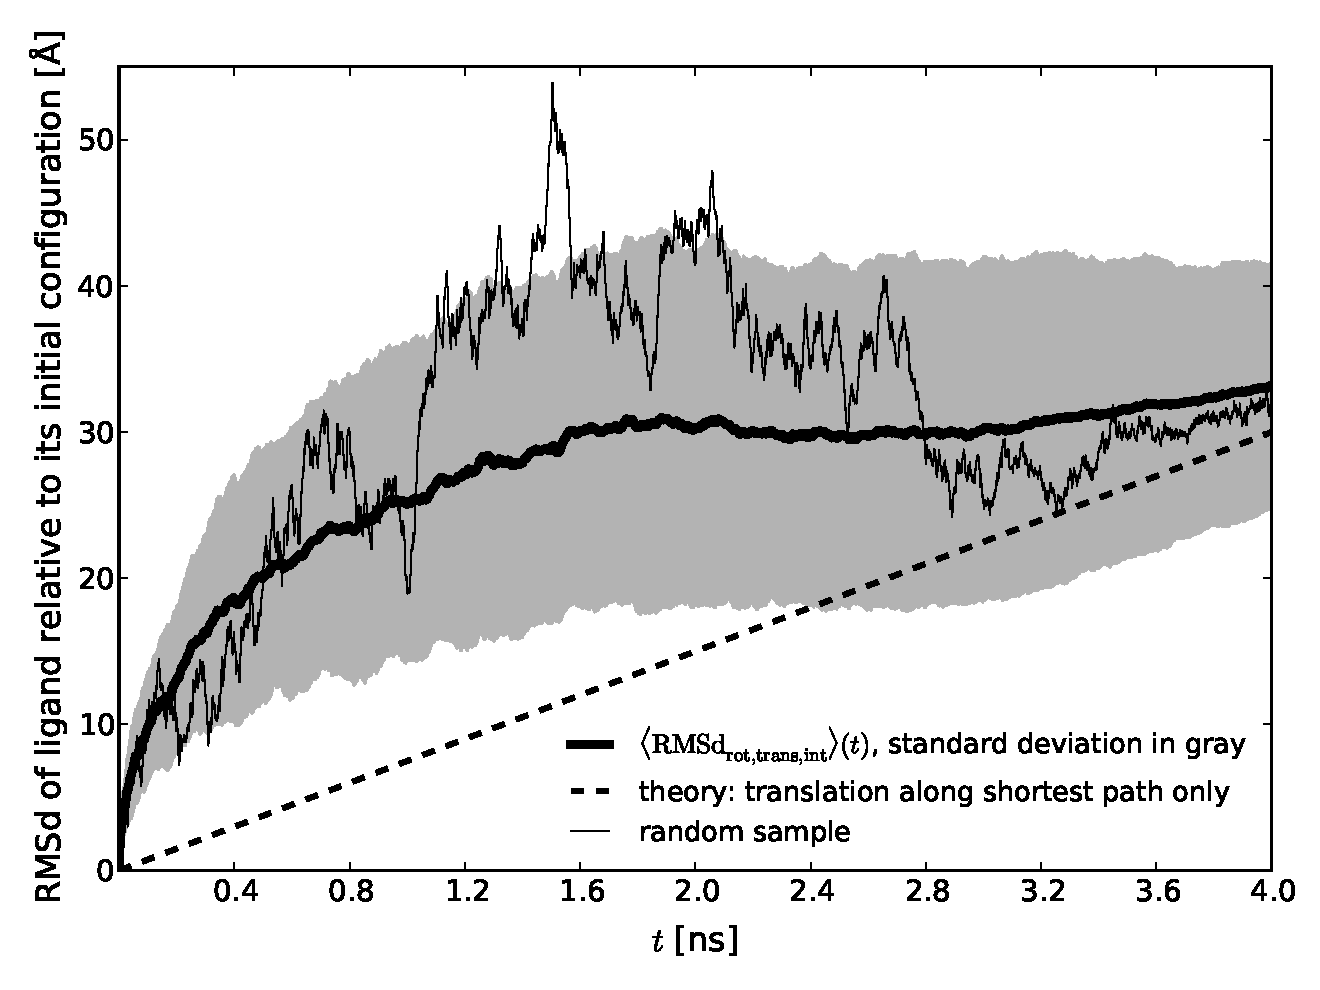
\includegraphics[width=1.0\textwidth]{gfx/dmd/figure_2_freedom_over_time_100samples_avg_stddev_randomone_pub_003.pdf}
\caption[]{
Translational and rotational freedom of a heparin tetramer while approaching
FGF2 during the tMD pulling process with $s=\SI{30}{\angstrom}$ and
\SI{4}{\nano\second}. For each point in time during tMD, the structural
difference between the current and initial ligand configuration was calculated
via classical $RMSd$ and averaged over 100 independent pulling processes. The
variation in ligand movement among different ligand trajectories is visualized
in terms of the standard deviation (grey background). }
\label{fig:dmd:sampling}
\end{figure}



For the FGF2-HP complex, we compared tMD runs with different pulling velocities
with the goal to find a moderate velocity which still allows significant
translational and rotational ligand movement. In such a case, entirely different
trajectories among tMD repetitions are produced so that Cartesian space sampling
as well as ligand orientation sampling can be enhanced by increasing the number
of tMD repetitions and leaving all other parameters constant. In tMD test runs
with varying duration $T$ but constant ligand displacement length $s$, we
measured the structural difference ($RMSd$) between the current and initial
ligand configuration for each point in time during tMD. Ligand translation,
rotation and internal conformational changes contribute to this time-dependent
structural difference denoted as $RMSd_{\mathrm{rot,trans,int}}(t)$.  The
difference $RMSd_{\mathrm{rot,trans,int}}(t) - ts/T$ describes the extent of
ligand translation and rotation in space compared to the shortest path scenario.

For single test cases with $T=\SI{4}{\nano\second}$ we observed a quickly
fluctuating $RMSd_{\mathrm{rot,trans,int}}(t)$ curve with ligand displacements
from the shortest path between 5 and \SI{40}{\angstrom} $RMSd$. In contrast,
when using $T=\SI{0.5}{\nano\second}$, the displacement varied in the range
between 0 and \SI{10}{\angstrom} $RMSd$. From these data, we could already
conclude that when using $T=\SI{4}{\nano\second}$, the limiting factor for
translational and rotational ligand sampling is the number of tMD repetitions
rather than the pulling velocity. To further quantify the translational and
rotational freedom of the ligand during tMD with $s=\SI{30}{\angstrom}$ and
$T=\SI{4}{\nano\second}$ in detail, we analyzed the deviation of the ligand from
the shortest path for an ensemble of 100 independent tMD runs. To this end, the
structural difference between current and initial ligand configuration was
calculated as described above and then averaged over all 100 independent pulling
processes for each point in time during tMD, leading to $\langle
RMSd_{\mathrm{rot,trans,int}}\rangle(t)$ (\cref{fig:dmd:sampling}). The average
extent of ligand translation and rotation in space turned out to have its
maximum at an $RMSd$ value of about \SI{20}{\angstrom}. The path variation among
ligand trajectories (the standard deviation of the averaged data) is about
$\pm\SI{10}{\angstrom}$ $RMSd$. The data suggest that with
$s=\SI{30}{\angstrom}$ and $T=\SI{4}{\nano\second}$ enough translational and
rotational freedom are provided to the ligand during tMD in order to be
applicable in a local docking method. This also verifies that the extend of
sampling of all ligand DOFs is determined and can be adjusted by the number of
tMD repetitions $N$.

$\langle RMSd_{\mathrm{rot,trans,int}}\rangle$ increases slower after about
$t=\SI{2}{\nano\second}$ (\cref{fig:dmd:sampling}), which is probably caused by
the electrostatic potential of the receptor prevailing against thermally driven
ligand movement. Having this transition included in the $\langle
RMSd_{\mathrm{rot,trans,int}}\rangle(t)$ curve is a good indication for a
properly (long enough) selected initial displacement length $s$. As a general
rule, $s$ should be chosen in a way that no atoms from the initially placed
ligand lie within the non-bonded interaction cut-off range of the receptor.

Due to the type of distance restraint applied, all final tMD states have the
central ligand atom positioned on the surface of the sphere given by the protein
core atom and the final restraint distance $D$. A more robust realization of the
basic DMD concept would not require assigning specific roles to certain points
(core atom and focus point) but implement a dynamic distance restraint between
receptor surface and ligand during the pulling process.

In the current setup, we have compensated for the spherical – and therefore
limited – distribution of tMD final ligand states via careful selection of the
core atom, of $D$, and via a long free MD simulation stage with
$T=\SI{10}{\nano\second}$. This allows for significant ligand refinement
according to the characteristics of the receptor surface as well as for an
exhaustive sampling of the internal DOFs of the ligand. We have quantified the
extent of glycosidic linkage sampling by analyzing the distribution of
glycosidic linkage dihedral values within all free MD simulations of a DMD study
with FGF2 in complex with heparin. Since GLYCAM 06 is known for its proper
description of the glycosidic linkage torsional
potential \cite{kirschner_glycam06:_2008}, we extracted the distribution of
equivalent torsion angles from an independently performed 760 ns MD simulation
of the same heparin molecule free in solution for reference. We compared both
distributions and observed high similarity between them
(\cref{fig:dmd:glycolinkage_sampling}). In particular, the distribution as
observed for the GAG-only simulation is entirely included in the distribution as
observed from the DMD MD simulations where the GAG is in contact with its
protein receptor. In the latter case, some additional conformers seem to be
accessible to the ligand when compared to the GAG-only simulation, which is to
be expected due to its interaction with the receptor. For further
characterization of the sampling, we extracted glycosidic linkage angle values
from 12 PDB entries containing free heparin as well as heparin-protein complexes
(1AXM, 1BFB, 1BFC, 1E0O, 1FQ9, 1G5N, 1GMN, 1HPN, 1QQP, 2AXM, 2HYU, 2HYV) and
observed that this range of experimentally determined angles is included within
the glycosidic torsion angle distribution as sampled by our MD simulations (also
shown in \cref{fig:dmd:glycolinkage_sampling}).


\begin{figure}
\begin{adjustwidth}{-1.5cm}{-1.5cm}
\centering
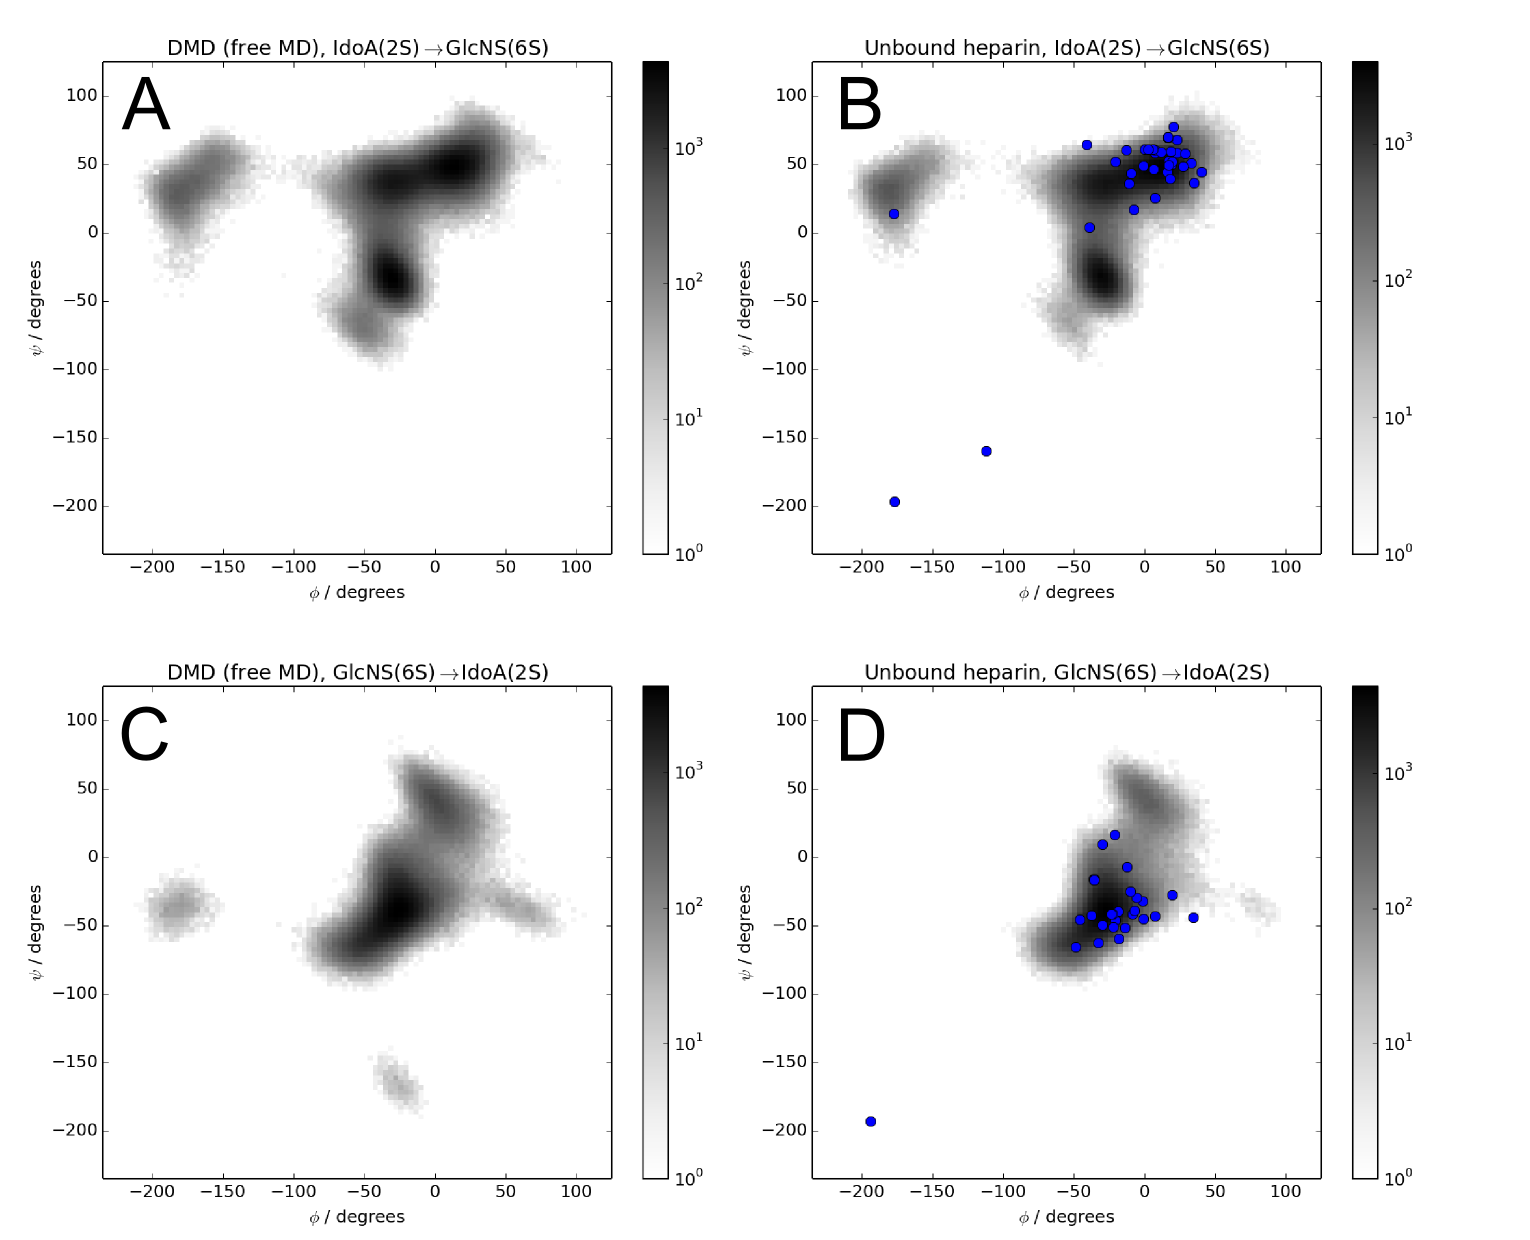
\includegraphics[width=1.3\textwidth]{gfx/dmd/suppl/suppl_glyco_linkage_torsion_maps_03.png}
\caption[]{
Conformational sampling of the glycosidic linkage dihedrals of a free (unbound)
heparin hexasaccharide extracted from 760 ns MD (B, D) compared to the sampling
in all free MD simulations in the DMD study of FGF2-HP (A, C). The torsion
angles are defined as follows: Φ is composed of the atomic chain H1-C1-O4-C4, Ψ
is composed of C1-O4-C4-H4, both in direction from the non-reducing end to the
reducing end of the GAG. All frequency distributions are shown in logarithmic
grey scale. The blue data points in panels B and D additionally show the
distribution of glycosidic linkage dihedral values of heparin as extracted from
the PDB entries 1AXM, 1BFB, 1BFC, 1E0O, 1FQ9, 1G5N, 1GMN, 1HPN, 1QQP, 2AXM,
2HYU, 2HYV (containing unbound as well as bound heparin molecules of different
lengths, the three outliers correspond to terminal sugar monomers).
}
\label{fig:dmd:glycolinkage_sampling}
\end{adjustwidth}
\end{figure}


Most important, we have observed that due to the long free MD stage and a large
number of DMD repetitions, the overall result of a DMD study becomes insensitive
to moderate changes in focus point coordinates as well as in the final tMD
restraint distance $D$.

When visualizing trajectories of tMD and free MD, we repeatedly observed
conceptually different scenarios. In one type of scenario, the ligand ended up
in its native binding pose in the final state of tMD. The conformation of the
ligand then did not undergo significant changes during free MD. In other cases,
the ligand arrived near its anchoring residues on the surface of the receptor
during tMD and then adopted the native binding mode within the free MD
simulation. We also observed the ligand to end up in a false-positive bound
state as well as in an unbound state after tMD or to unbind during free MD.

From these observations we can deduce that if after DMD no agglomeration of
docking solutions stands out, the chosen receptor target region most likely does
not contain a real binding site for the ligand. Furthermore, even if the focus
point of the method is not centered on but only in the vicinity of a real
binding site, the latter most likely stands out during data analysis.

\subsubsection{DMD performance}

\begin{figure}
\centering
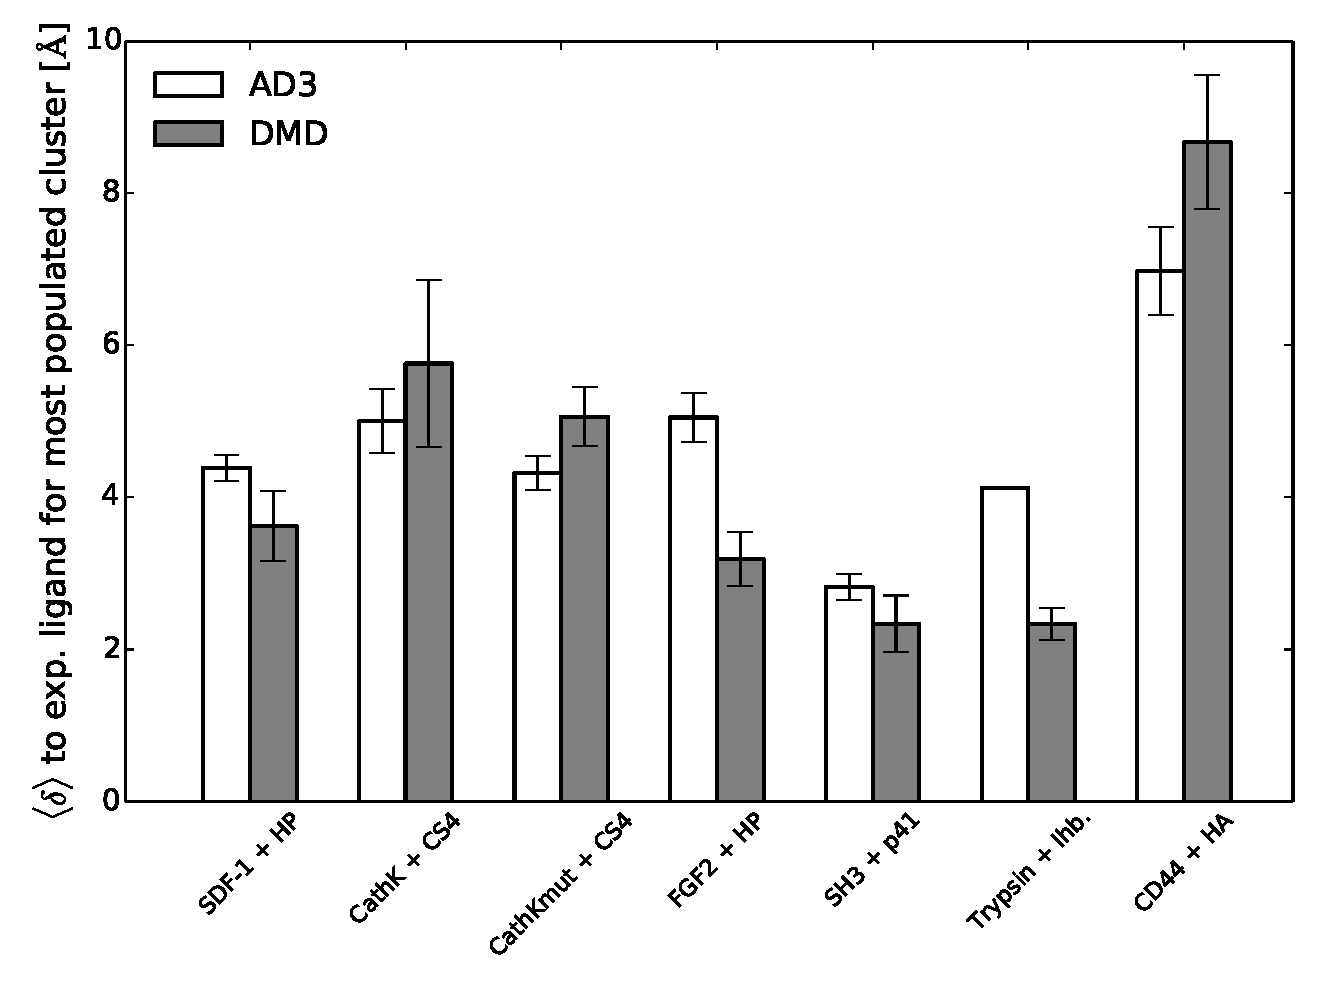
\includegraphics[width=0.9\textwidth]{gfx/dmd/figure_4_clustering_dmd_vs_ad3_plots_pub_004.pdf}
\caption[]{
Mean structural distance $\langle \delta \rangle$ between all members of the
most populated cluster and the experimentally determined ligand for all
investigated complexes with both docking methods. The error bars show the
standard deviation of the mean.
}
\label{fig:dmd:clus_dmd_vs_ad3}
\end{figure}



\begin{table}
\tiny
\centering
\renewcommand{\arraystretch}{1.3}
\begin{tabular}{@{}lcccc@{}}
\multicolumn{5}{c}{\textbf{DMD}} \\
\midrule
Complex & $\epsilon$ / \si{\angstrom} & members & $\delta$ / \si{\angstrom} (mean) &  $\delta$ / \si{\angstrom} (std. dev.) \\
\midrule
CathKmut + CS4 & 3.0 & 6   & 5.1 & 0.4 \\
CathK + CS4    & 3.0 & 4   & 5.8 & 1.1 \\
SDF1 + HE      & 2.2 & 8   & 3.6 & 0.5 \\
CD44 + HA      & 3.2 & 5   & 8.7 & 0.9 \\
SH3 + p41      & 2.6 & 8   & 2.3 & 0.4 \\
FGF + HE       & 2.5 & 6   & 3.2 & 0.4 \\
Trypsin + Ihb. & 1.0 & 9   & 2.3 & 0.2 \\
\midrule
& & & & \\
\multicolumn{5}{c}{\textbf{AD3}} \\
\midrule
Complex & $\epsilon$ / \si{\angstrom} & members & $\delta$ / \si{\angstrom} (mean) &  $\delta$ / \si{\angstrom} (std. dev.) \\
\midrule
CathKmut + CS4  & 2.5 & 6   & 4.3 & 0.2 \\
CathK + CS4     & 2.0 & 9   & 5.0 & 0.4 \\
SDF1 + HE       & 1.2 & 19  & 4.4 & 0.2 \\
CD44 + HA       & 2.5 & 8   & 7.0 & 0.6 \\
SH3 + p41       & 1.8 & 10  & 2.8 & 0.2 \\
FGF + HE        & 1.6 & 10  & 5.1 & 0.3 \\
Trypsin + Ihb.  & 0.1 & 100 & 4.1 & 0.0 \\
\midrule
\end{tabular}
\caption{
Clustering parameters of the most populated cluster for docking solution
ensembles obtained via DMD and AD3. $\epsilon$ is the neighborhood search radius
as used for DBSCAN clustering, $\delta$ measures the structural difference
between two molecules (see Methods).
}
\label{tab:dmd:clustering_parameters}
\end{table}


\vspace{1cm}
\textbf{Spatial distribution of docking solutions.}
We compared the performance of DMD with the performance of the well-established
AD3 docking approach, which was used for other molecular systems including GAGs.
We applied DMD and AD3 to all TDS complexes and analyzed the spatial
distribution of docking results via clustering
(see \cref{tab:dmd:clustering_parameters}). For each
complex, we compared the mean structural distance $\langle \delta \rangle$
between the experimentally determined ligand position and all members of the
most populated cluster (\cref{fig:dmd:clus_dmd_vs_ad3}). In terms of the
capability to produce solutions structurally close to the experimentally
determined ones, both docking methods perform comparably well. However,
interesting differences are observable. AD3 generally yields smaller spatial
scattering of solutions as given by the standard deviation of data points in
\cref{fig:dmd:clus_dmd_vs_ad3}. This can be attributed to the static treatment
of the receptor by AD3. Notably, we can generally conclude that DMD performed
better than AD3 for the complexes with strongest electrostatic attraction,
namely SDF-1-HP and FGF2-HP. For the FGF2-HP complex, the most populated cluster
from DMD reproduces the experimentally determined HP binding pose, while the
most populated cluster from AD3 docking only partially overlaps with this pose
(\cref{fig:dmd:fgf2zoom}a). In fact, DMD was able to identify the
\enquote{higher affinity} binding site for heparin (as denoted in the original
publication of the FGF2-HP crystal structure), while AD3 identified the
\enquote{lower affinity} site, which becomes occupied upon heparin
hexasaccharide binding \cite{faham_heparin_1996}. In addition, DMD was able to
properly predict the positioning of the two sulfate groups making specific high-
affinity contact to FGF2 (\cref{fig:dmd:fgf2zoom}b). These two sulfate groups
form seven of the nine polar contacts between FGF2 and HP and therefore are
important anchoring groups for the molecular recognition
\cite{faham_heparin_1996}. The fact that DMD was able to reproduce this key
feature as opposed to AD3 most probably reflects the crucial role of receptor
flexibility considered in the docking simulation.

\begin{figure}
\centering
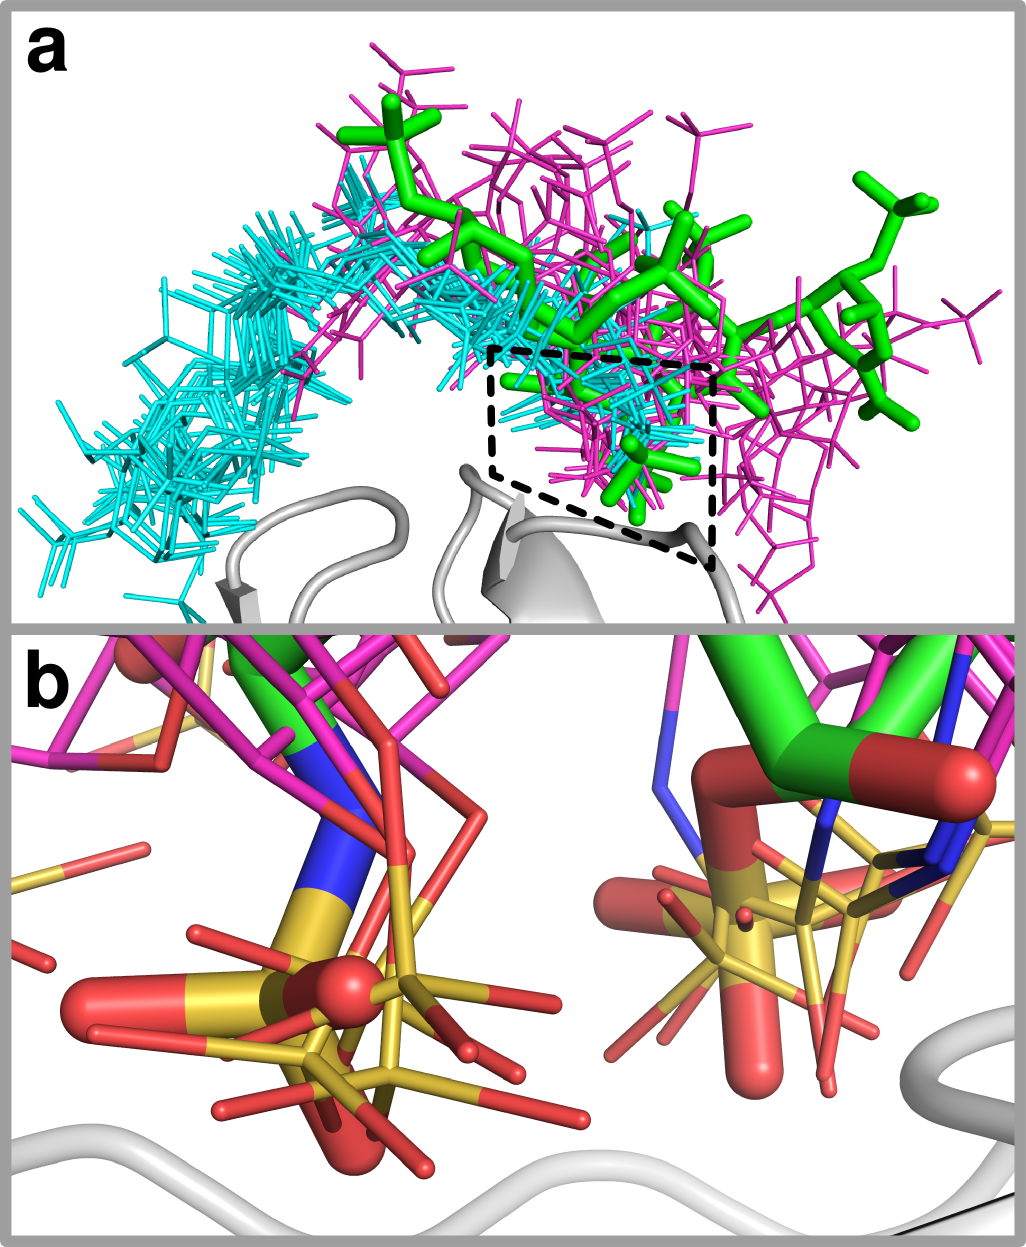
\includegraphics[width=0.9\textwidth]{gfx/dmd/fgf2_topclusters_dmd_vs_ad3_receptorribbon_normal_and_zoom_jcc_004.png}
\caption[]{
Docking results from DMD and AD3 for FGF2 (grey cartoon representation) and HP.
\textbf{a}: ligand from crystal structure in green sticks. Most populated
cluster of DMD solutions in magenta. Most populated cluster of AD3 solutions in
cyan. \textbf{b}: zoom on two sulfate groups making specific high-affinity
contact to FGF2 \cite{faham_heparin_1996} (as marked in \textbf{a} via dashed
line). Ligand from crystal structure with C atoms in green (thick sticks). Most
populated DMD cluster with C atoms in magenta (thin sticks).
}
\label{fig:dmd:fgf2zoom}
\end{figure}


In order to assess the ability of DMD to predict consistent binding poses for
GAGs differing in length, we carried out additional DMD studies for SDF-1 as
well as FGF2. Eventually, both systems were investigated with independent DMD
studies for each of di-, tetra- and hexasaccharides of heparin. For FGF2-HP, the
two sulfate groups making specific contact to FGF2 were identified when docking
both an HP tetrasaccharide and an HP hexasaccharide. These observations support
the assumption that GAG fragments differing in length share key interactions
with the protein. When docking an HP disaccharide, those key interactions were
not identified, suggesting that the disaccharide is not long enough to maintain
specificity. Nevertheless, for the SDF-1-HP and FGF2-HP systems, we observe that
all obtained poses overlap regardless of the GAG length
(\cref{fig:dmd:fgf2_hp_246,fig:dmd:sdf1_hp_246}).  A direct visual comparison
between the crystal structure of FGF2 with a heparin
hexasaccharide \cite{faham_heparin_1996} and the corresponding DMD result can
be seen in \cref{fig:dmd:fgf2_hp_246}.


\begin{figure}
\centering
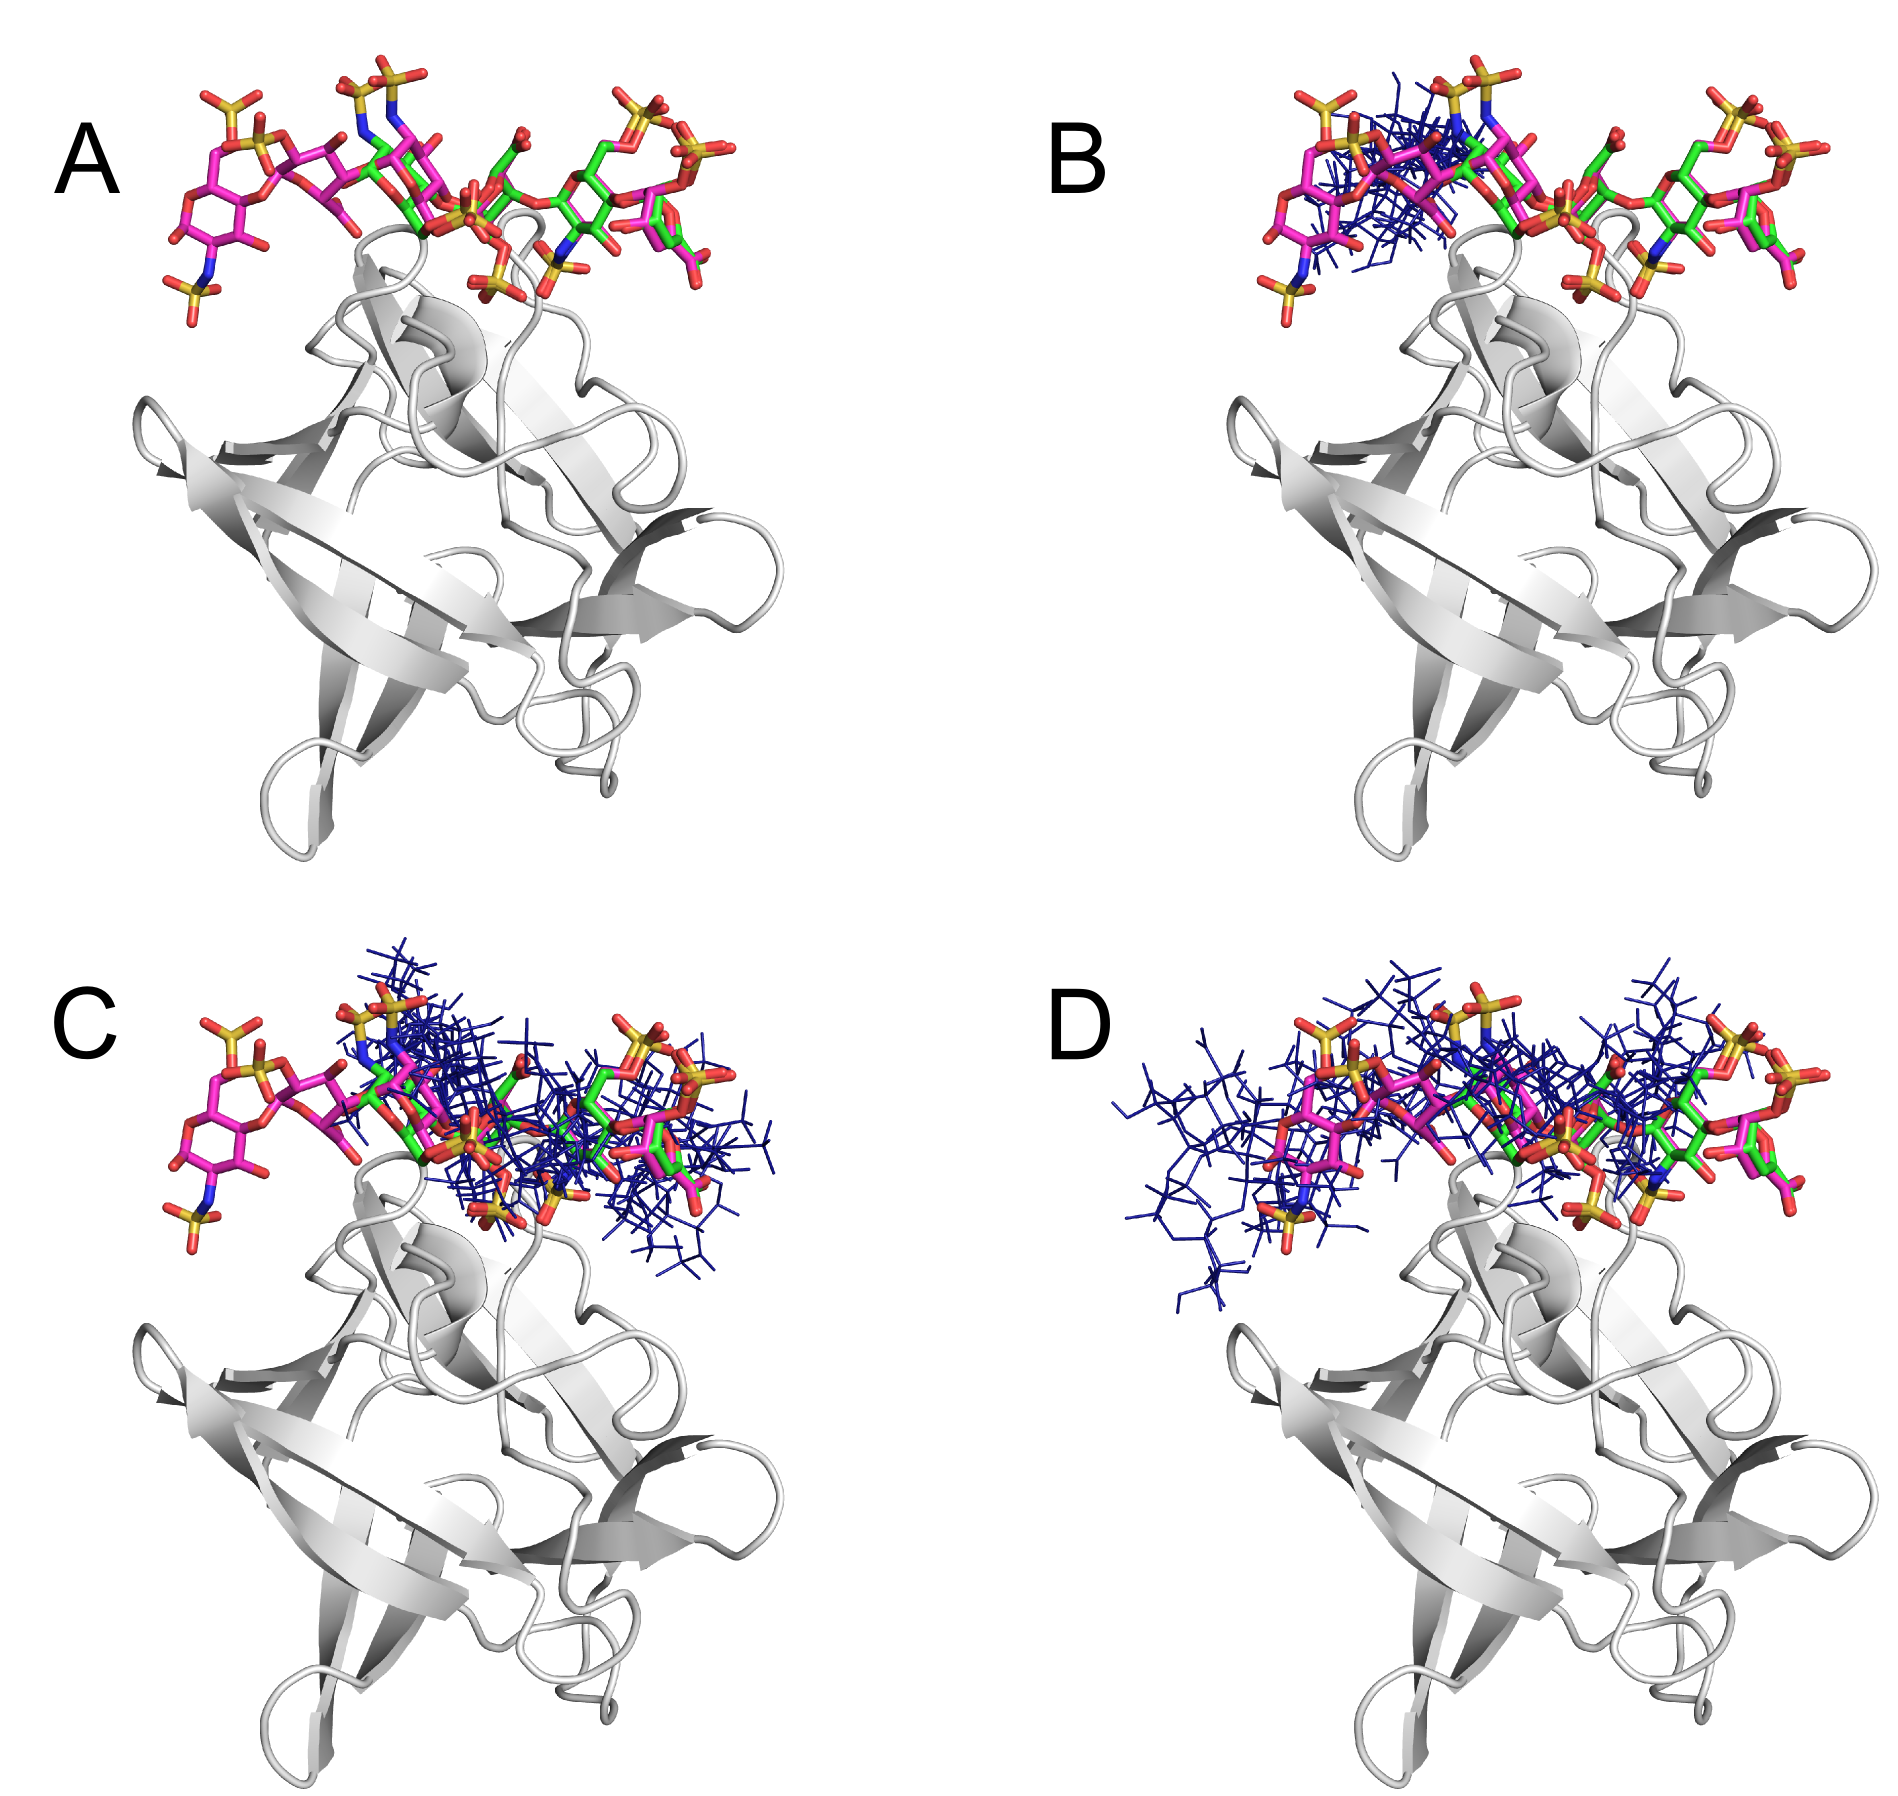
\includegraphics[width=0.9\textwidth]{gfx/dmd/suppl/suppl_fgf2_dmd_he-2-4-6_02.png}
\caption[]{
DMD results for FGF2 in complex with a heparin di-, tetra- and hexasaccharide.
In magenta and green sticks, the heparin hexamer and tetramer poses as
determined experimentally are shown (PDB IDs 1BFB, 1BFC), respectively. The most
populated clusters for di-, tetra- and hexasaccharide docking solutions are
shown in B, C, D, respectively, as blue sticks. The protein is shown in grey
cartoon.
}
\label{fig:dmd:fgf2_hp_246}
\end{figure}


\begin{figure}
\centering
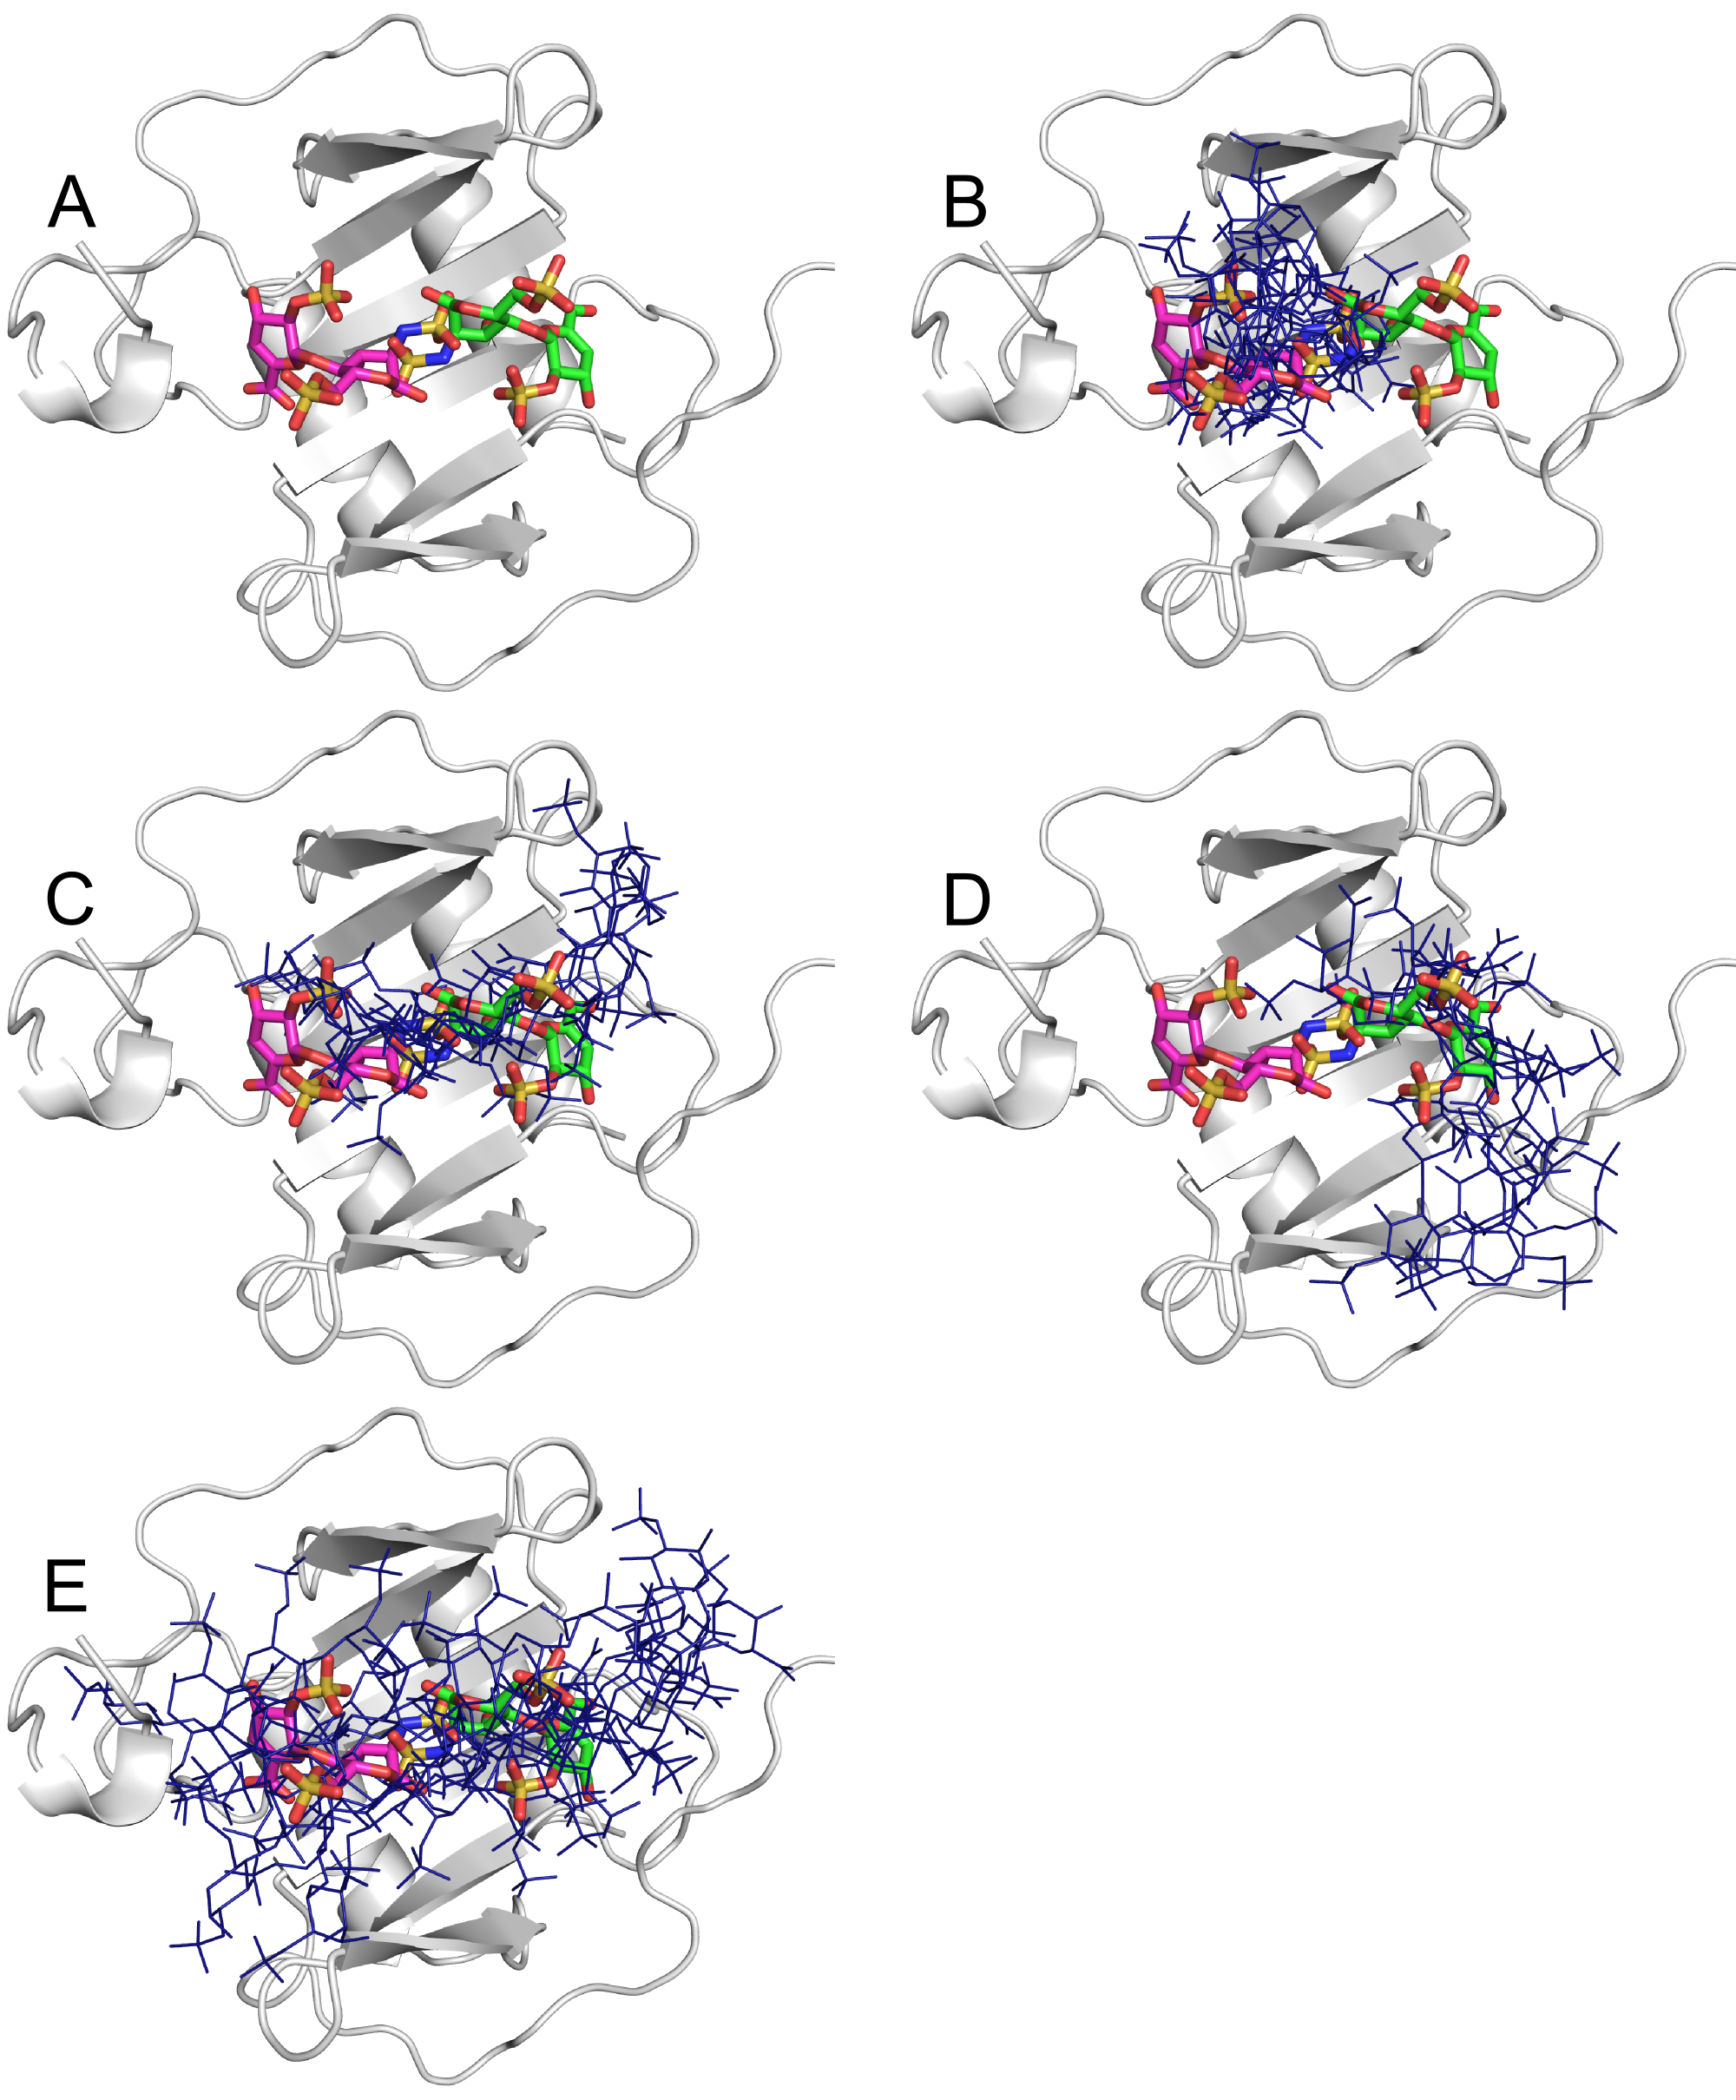
\includegraphics[width=0.9\textwidth]{gfx/dmd/suppl/suppl_sdf1_dmd_he-2-4-6.png}
\caption[]{
DMD results for SDF-1 in complex with a heparin di-, tetra- and hexasaccharide.
In magenta sticks, the heparin dimer pose as determined experimentally is shown
(PDB ID 2NWG). For clarity, we show its symmetric counterpart (180 degree
rotation about the 2-fold axis of the SDF-1 dimer) in green sticks. The most
populated clusters for di-, tetra- and hexasaccharide docking solutions are
shown in B, C \& D, E, respectively, as blue sticks. The protein is shown in
grey cartoon.
}
\label{fig:dmd:sdf1_hp_246}
\end{figure}


As has been conceptually described for the FGF2-HP complex, also regarding the
SH3-p41 and Trypsin-inhibitor complexes, DMD provided solutions closer to the
experimentally determined ones while displaying a more diverse scattering of
docking solutions than AD3.

For CD44 in complex with the HA heptamer, both docking methods were only
partially able to reproduce the experimentally determined ligand pose. Weak net
electrostatic repulsion between receptor and ligand seemingly imposes a major
challenge for both docking methods. AD3 and DMD solutions, however, are
spatially consistent (data not shown).

Both docking methods had difficulties reproducing the experimentally determined
binding poses of CathK and CathKmut in complex with CS4. In case of CathK-CS4,
the crystal structure contains a single high molecular weight polymeric CS4
molecule interacting with multiple copies of the same protein
\cite{catK_cs4_crystal_structure_2008}. Within the CathKmut-CS4 crystal, each
GAG hexamer tightly interacts with two CathKmut proteins
\cite{catKmut_cs4_crystal_2011}. Under these conditions, it is to be expected
that considering only a short GAG and a single protein in the docking experiment
is not sufficient to allow for an accurate reproduction of the experimentally
determined structures.

The presented structural difference comparison between DMD and AD3-based docking
solutions and the corresponding experimentally determined ligand coordinates is
subject to a systematic error. Structural relaxation prior to docking with AD3
changed the receptor side chains in the binding region by a heavy atom $RMSd$ of
\SI{1.0 +- 0.4}{\angstrom} (mean value and standard deviation derived from all
TDS complexes) when compared to the experimentally determined receptor
structure. The solutions from DMD display a mean binding region alteration of
\SI{2.3 +- 0.6}{\angstrom} (corresponding raw data is shown in
\cref{tab:dmd:binding_site_rmsd}). The larger the binding site alteration, the
more error-prone the comparison between docked solution and experimentally
determined ligand becomes. Under the assumption that this error systematically
increases the structural difference, DMD might have performed better compared to
AD3 than shown in Figure 4.


% http://www.inf.ethz.ch/personal/markusp/teaching/guides/guide-tables.pdf
\begin{table}
\tiny
\centering
\renewcommand{\arraystretch}{1.3}
\begin{tabular}{@{}lcccc@{}}
\toprule
& \multicolumn{2}{c}{\textbf{DMD (after free MD)}} & \multicolumn{2}{c}{\textbf{AD3}} \\
Complex & Entire receptor & Binding site &  Entire receptor & Binding site \\
\midrule
SDF-1 + HP & 3.6 $\pm$ 0.5 & 2.3 $\pm$ 0.5 &  0.4 & 0.2 \\
CathK + CS4 & 1.8 $\pm$ 0.2 & 2.0 $\pm$ 0.3 & 1.1 & 1.2 \\
CathKmut + CS4 & 1.8 $\pm$ 0.2 & 1.9 $\pm$ 0.4 & 1.1 & 1.4 \\
FGF2 + HP & 3.4 $\pm$ 0.1 & 3.6 $\pm$ 0.1 & 1.3 & 1.1 \\
SH3 + p41 & 2.2 $\pm$ 0.2&  2.4 $\pm$ 0.4 &  1.3 & 1.4 \\
Trypsin + Ihb. & 1.6 $\pm$ 0.1 & 1.5 $\pm$ 0.4 & 0.9 & 0.7 \\
CD44 + HA & 2.2 $\pm$ 0.3 & 2.5 $\pm$ 0.5 & 0.9 & 0.7 \\
\bottomrule
\end{tabular}
\caption{
Heavy atom RMSd between experimentally determined structure of the receptors and
the receptor structures corresponding to the docking solutions. Differences were
obtained for \textit{i} the entire receptor and \textit{ii)} the binding site
only as determined by the MOE \enquote{pocket} feature. In case of DMD, mean
distances $\pm$ standard deviation were obtained from 100 independent free MD
runs per complex. Numbers are given in ångströms.
}
\label{tab:dmd:binding_site_rmsd}
\end{table}

\vspace{1cm}
\textbf{Identification of anchoring residues in the ligand binding
region.} The prediction of receptor residues important for ligand binding is of
particular practical value. While AD3 does not provide energetic data on the
single-residue level, DMD allows for a single-residue energy decomposition
(SRED) based on time-averaged free MD interaction energy data.

For each TDS complex, we merged SRED data from the entire ensemble of DMD runs
and extracted the set of anchoring residues, which are at most ten of the
receptor residues contributing most (positively) to ligand binding. We also
determined a reference set of anchoring residues from MD simulations of the
experimentally determined structures. For each TDS complex, we then identified
the intersection of both sets (\cref{tab:dmd:anchoring_receptor_redidues}).


\begin{table}
\tiny
  \centering
  \smallskip
  \begin{threeparttable}
    {\renewcommand{\arraystretch}{1.3}%
      \begin{tabular}{lcccr}
      \hline
      \textbf{Complex} & \specialcell{\textbf{Number of correctly} \\ \textbf{predicted residues}\tnote{a}} &
      \specialcell{\textbf{Number of} \\ \textbf{charged residues}} &
      \specialcell{\textbf{Number of polar} \\ \textbf{uncharged residues}} & $r$\tnote{b} \\ \hline
      SDF-1 + HP & 7 of 10 & 7 & 0 & 0.52 \\
      CathK + CS4 & 6 of 10 & 4 & 2 & -0.21 \\
      CathKmut + CS4 & 6 of 10 & 4 & 1 & -0.12 \\
      FGF2 + HP & 9 of 10 & 6 & 2 & 0.84 \\
      SH3 + p41 & 2 of 5 & 0 & 0 & -- \\
      Trypsin + Ihb. & 5 of 10 & 2 & 2 & 0.73 \\
      CD44 + HA & 1 of 7 & 1 & 0 & -- \\ \hline
      \end{tabular}
    }
    \begin{tablenotes}
      \item[a] Number of predicted receptor anchoring residues having a match in
      the reference set (as obtained from SRED via MD of the experimentally determined structures).
      \item[b] Spearman's rank correlation $r$ between the SRED-energies of both residue sets
      (calculated only if five or more residues match).
    \end{tablenotes}
  \end{threeparttable}
\caption{Predictive power of DMD for the identification of receptor anchoring residues.}
\label{tab:dmd:anchoring_receptor_redidues}
\end{table}


For Trypsin in complex with its inhibitor, half of the anchoring residues in the
crystal structure were correctly found. For SDF-1-HP, CathK-CS4, and
CathKmut-CS4 more than half of the anchoring residues were identified by SRED.
Furthermore, for the FGF2-HP complex, nine of ten anchoring residues were
predicted properly.

In order to evaluate the capability of DMD to rank the receptor anchoring
residues according to their importance for ligand binding, we calculated
Spearman's rank correlation between the SRED-energies of residues in both, the
reference and comparison sets (\cref{tab:dmd:anchoring_receptor_redidues}). For
three of those five complexes with at least five predicted anchoring residues,
the DMD ranking turned out to reproduce the reference ranking quite well
(SDF-1-HP, FGF2-HP, Trypsin-Ihb). For the CathK-CS4 and CathKmut-CS4 complexes
the anchoring residue ranking was not reproduced.

\begin{figure}
\centering
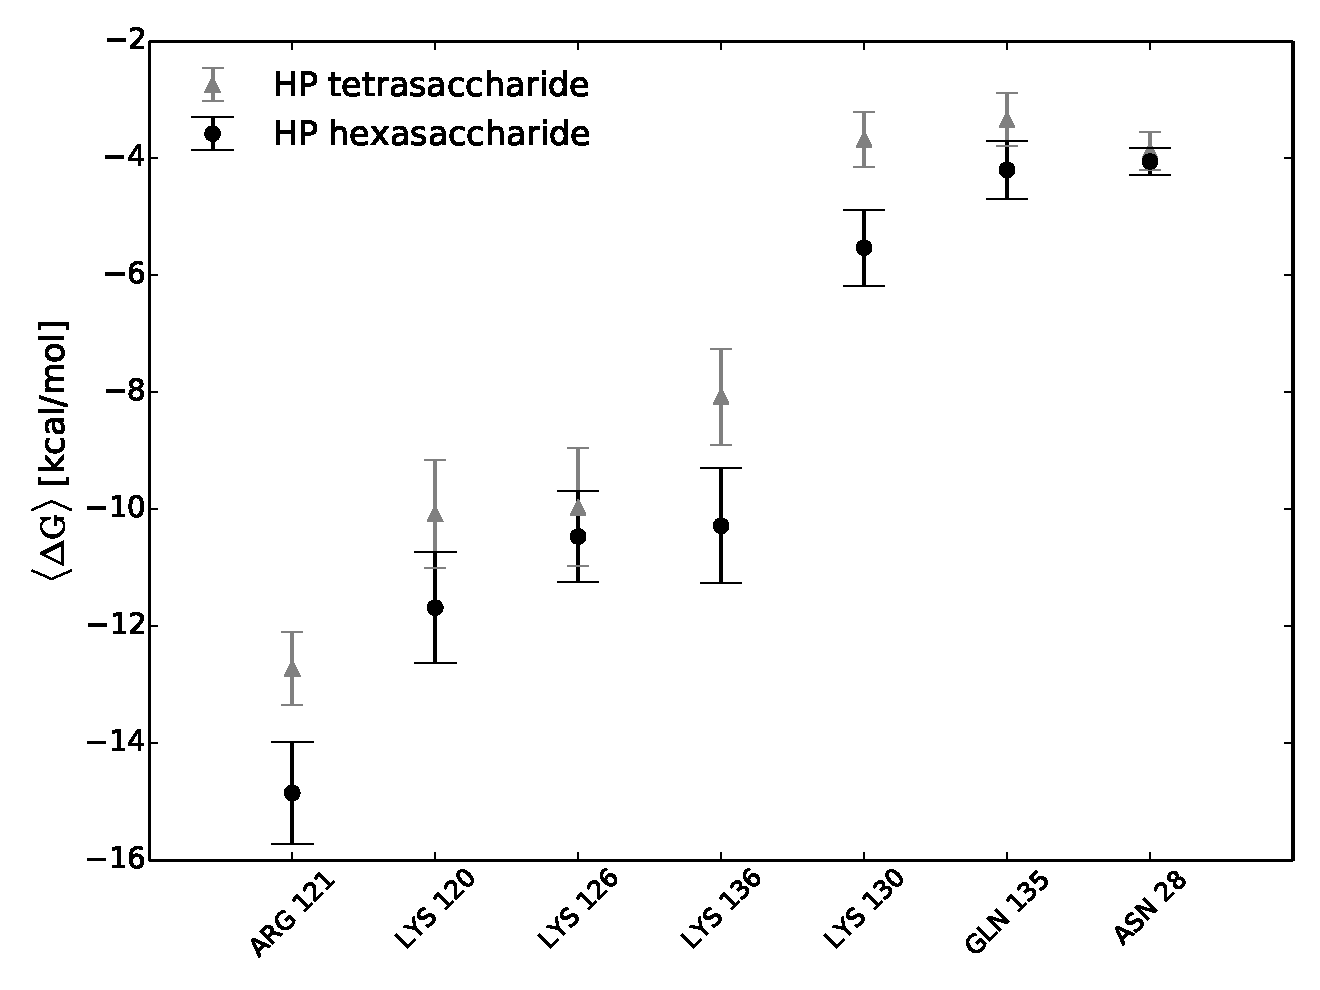
\includegraphics[width=1.0\textwidth]{gfx/dmd/figure_6_receptor_top7_residues_of_top_40percent_dmd_runs.pdf}
\caption[]{
FGF2 amino acid residues identified by DMD as having the greatest impact on
FGF2-HP binding. Results are shown for both heparin tetra- and hexasaccharide
ligands as retrieved from two independent DMD studies. For each residue, an
average energy ($\pm$ standard error of the mean) for the interaction with the
ligand is shown as obtained from 40 independent free MD simulations.
}
\label{fig:dmd:sred_fgf2}
\end{figure}

Based on the obtained results, we can conclude that for systems dominated by
electrostatic attraction such as protein-GAG systems, DMD is capable of
correctly identifying those amino acid residues responsible for forming key
interactions with the ligand. Regarding the FGF2-HP system, we found that both
heparin tetra- and hexasaccharide docking via DMD enabled us to consistently
identify the same chemical groups in the GAG molecule being key for binding.
Moreover, using SRED data, we were able to demonstrate that the identified key
amino acid residues as well as their energy ranking are identical when comparing
heparin tetra- and hexasaccharide docking performed in independent DMD studies
(see \cref{fig:dmd:sred_fgf2}). This observation supports the idea that,
regardless of their length, GAG fragments preserve their key interactions with
certain protein amino acid residues. The set of FGF2 key amino acid residues as
identified by SRED contains all residues that were crystallographically
characterized as most important for binding (R121, K126, N28,
Q135) \cite{faham_heparin_1996}. Based on our data we can additionally state
that also residue K120 is of major importance, since it acts as hydrogen bond
donor in a similar way as K126 does. The latter observation is in agreement with
previous calorimetry studies pointing out the importance of K120 in the FGF2-HP
system \cite{thompson_1994_fgf2_heparin}. These findings motivate the
application of DMD to systems in which a detailed and appropriate description of
GAG recognition is required.



\subsubsection{Electrostatic potential analysis in the context of DMD}

Our electrostatic potential evaluation procedure as discussed in
\cref{chapter:bspred} unambiguously identifies the GAG binding sites as
determined experimentally for SDF-1-HP as well as the FGF2-HP systems. Analysis
of CD44's Coulomb potential revealed that the net electrostatic interaction
between CD44 and HA is either insignificant or even slightly repulsive. These
findings seem to be directly correlated to the success of DMD in terms of
reproducing the natural ligand binding mode, which can be described as failure
in case of the CD44-HA system. We observe that electrostatic potential analysis
provides a clear idea whether GAG-binding to a given receptor is mainly driven
by Coulomb interaction. If a protein is known to bind GAGs, and the
electrostatic potential topology is as unambiguous as in case of SDF-1 or FGF2,
a GAG binding site prediction based on the procedure presented in
\cref{chapter:bspred} is reliable and can be used for planning a DMD study for a
given system. Visualization of the electrostatic potential can in any case be
helpful to \textit{a priori} exclude regions of the receptor surface when
repulsive to negatively charged ligands. Especially, knowledge about the
electrostatic potential distribution in space can be used to choose a reasonable
ligand \enquote{entry lane} orientation for the tMD pulling process.


\subsubsection{General discussion}

In summary, our data suggest that DMD is able to yield docking results of high
significance, especially in case of receptor-ligand systems dominated by
attractive electrostatic interaction. This success is well-grounded by the
concept that the ligand --- while slowly approaching the receptor surface ---
performs extensive conformational sampling and, at the same time, responds to
the long-range Coulomb potential of the receptor. During the pulling process,
the Coulomb potential significantly contributes to steering the entirely
flexible and charged ligand towards its binding site and to let it finally adopt
its binding pose in an explicit solvent environment. The subsequent free MD step
allows for an unbiased mutual adjustment of receptor residues and ligand.

DMD is a local docking method focused towards a certain region on the receptor
surface. When selecting focus point, core atom, and target distance $D$, one
needs to ensure that after the pulling process, the ligand is able to establish
short-range interactions within the receptor binding region but is not forced
into clashes with the receptor. In our study, we selected the focus point based
on the experimentally determined ligand position and could therefore easily
determine the required MD target distance values
(\cref{tab:dmd:tds_target_distances}). In practice, when the structure of the
bound ligand is unknown, the focus point has to be defined based on the residues
comprising the putative binding region and based on binding mode assumptions,
for instance generated by classical docking methods or by manual docking .

\begin{table}
\scriptsize
\centering
\renewcommand{\arraystretch}{1.3}
\begin{tabular}{@{}lr@{}}
\toprule
Complex & $D$ / \si{\angstrom} \\
\midrule
SDF-1 + HP & 10.6 \\
CathK + CS4 & 19.2 \\
CathKmut + CS4 & 20.9 \\
FGF2 + HP & 25.0 \\
SH3 + p41 & 7.7 \\
Trypsin + Ihb. & 12.1 \\
CD44 + HA & 15.3 \\
\bottomrule
\end{tabular}
\caption{
Target distance $D$ as applied during the tMD simulations for any given TDS complex.
}
\label{tab:dmd:tds_target_distances}
\end{table}


One of the main concepts of DMD is that pulling process and subsequent free MD
are repeated many times in independent simulations. This allows for the creation
and evaluation of an ensemble of docking solutions rather than the
interpretation of single trajectories. In this ensemble, the energetically more
favorable states are the more likely ones. Spatial clustering of this docking
solution ensemble identifies those docking solutions that appeared with highest
probability and, therefore, lowest energy. With respect to the identification of
anchoring residues in the receptor and their energetical ranking, meaningful
results can be obtained by merging the properties of multiple docking solutions.

Sampling performance is one of the main limitations of any docking method.
Regarding our DMD protocol applied to the TDS complexes, we have shown that with
100 independent DMD runs the sampling performance was sufficient for generating
meaningful docking solution ensembles. Although the predictive significance of
DMD in this study has been good enough, it can still be largely improved by a
sampling enhancement. An obvious way for achieving this would be to increase the
number of independent DMD runs, which would result in an even clearer picture
upon clustering of a docking solution ensemble. Furthermore, the current DMD
protocol leaves room for optimizing the sampling performance per compute time
via careful reduction of the ligand starting distance and increase of the
pulling velocity.

Regarding the overall reliability of the data produced by DMD one of the most
important results is the agreement of the ensemble-derived SRED data obtained
from two independently performed DMD studies (see \cref{fig:dmd:sred_fgf2}).
This agreement is a strong indicator for overall convergence, which in turn
is the requirement for the reliable interpretation of data obtained from
molecular dynamics simulations. Another important aspect to discuss in terms
of reliability is that in our in-house tests we have seen that the outcome
of a DMD study does not too strictly depend on special DMD parameters such as
the target distance.

Beyond the proof of concept provided by this study for including receptor
flexibility and explicit solvent in molecular dynamics-based docking of
protein-GAG systems, the analysis of MD data collected in the course of DMD can
be largely extended to further increase the atomic resolution of results,
improve the overall predictive significance and to gain new insights into
molecular recognition mechanisms. The behavior and role of single water
molecules in ligand binding, for instance, could be investigated thoroughly.
Furthermore, the dynamic nature of DMD data enables and motivates the creation
of specialized scoring schemes, e.g.\ the evaluation of ligand position
fluctuations during free MD as an indicator for the stability of a docking
solution. Also, the single-residue energy decomposition analysis can be
accompanied by an evaluation of hydrogen bond formation and occupancy via simple
distance and angle criteria.

An important challenge in GAG-protein docking is to properly deal with the
conformational flexibility of IdoA(2S) in heparin
\cite{Mulloy_dyn_conf_heparin_2000, barbero_jacs_2005}. Unfortunately, GLYCAM 06
is known to not properly reproduce the natural ring conformer population of
IdoA(2S) \cite{gandhi_idoa2s_2010} and its ring conformation interconversion
time scale is beyond simulation times accessible in DMD anyway
\cite{almond_jacs_2010}. Nevertheless, this issue can be addressed by applying
ring-internal restraints to explicitly impose a certain conformation on
individual rings (as outlined in the Methods section) and then perform a number
of independent DMD studies differing only in the combination of ring
conformations -- an approach which has recently been proposed by Muñoz-García
and co-workers {\cite{conf_idoa_timeavg_restraints_2013}}. As we have shown
previously, the MM-PBSA approach is capable of distinguishing GAG poses
differing only in the conformation of one single ring
\cite{Samsonov_rings_cr_2013}.

Although the computational demands for DMD are higher than for conventional
docking methods such as AD3, investigations of single systems via DMD are
entirely feasible when having access to reasonable computing resources,
especially using MD software optimized for GPU hardware such as Amber: a DMD
study for the FGF2-HP complex as presented here can be performed within one week
incorporating six modern GPU cards (GTX 580 in this case).

\subsection{Conclusions}

In this study, we have established and tested DMD, a targeted molecular
dynamics-based protocol for local docking developed for specifically tackling
the challenges imposed by highly flexible systems dominated by electrostatic
interaction, such as protein-GAG systems.

In particular, flexible treatment of the receptor copes with the fact that GAGs
usually bind to charged surface patches on the receptor comprised of highly
flexible side chains. The identification of proper binding poses in these
surface patches requires the flexible adjustments of protein residues to the GAG
ligand. Furthermore, the inclusion of explicit solvent in DMD considers the
solvent-accessibility of such binding sites and -- most important -- lives up to
the supremacy of charge-charge interactions in most protein-GAG complexes. The
dominating long-range Coulomb potential is explicitly exploited as a driving
force in DMD while slowly approaching the ligand towards the receptor. A long
free MD simulation and the flexible treatment of the ligand allow for an
extensive sampling of the GAG-internal degrees of freedom.

We show that DMD has high predictive significance for systems dominated by
electrostatic attraction. Our data implicate that via proper selection of DMD
parameters such as pulling velocity, ligand displacement distance and the number
of independent repetitions, sufficient sampling is achievable. We demonstrate
that in some cases the simple analysis of the spatial distribution of the
electrostatic potential of the receptor can lead to a reliable prediction of the
GAG binding region and therefore offers itself as a useful tool for defining the
target region on the receptor surface as required by DMD.

Regarding the spatial distribution of docking solutions, DMD generally yields
results comparable to AD3. Nevertheless, DMD performs better in terms of
achieving agreement with atomic details inferred from experimental data. The
time-dependent data obtained via DMD allows for a reliable prediction of
receptor anchoring residues via MM-PB(GB)SA single-residue energy decomposition,
yielding consistent results when docking GAGs of different length. Furthermore,
obtained MD trajectory data pave the way for the evaluation of various
dynamics-based measures, the development of specialized scoring schemes, and the
investigation of the dynamic nature of molecular interaction mechanisms within a
particular system.

\chapter{DMD applied to the IL-10-GAG system}

The previous chapter presented Dynamic Molecular Docking (DMD), a novel
molecular dynamics-based local docking method that was shown to be well-suited
for exploring protein-GAG interaction. Subsequently, I applied DMD to the
IL-10-GAG system and utilized the previous achievements presented in this thesis
--- the binding region prediction derived in \cref{chapter:bspred} and the
clustering methodology presented in \cref{chapter:clustering}.

The objective of applying DMD to the IL-10-GAG system was to discover molecular
details about the fundamental paradigm governing IL-10-GAG interaction, limited
to the putative IL-10-GAG binding region presented in \cref{chapter:bspred}. In
other words, while the rational considerations made in \cref{chapter:bspred}
lead to a certain molecular interaction model of low spatial resolution, the
work presented in this chapter seeks to reveal further detail, based on
extensive sampling of the dynamics of the system. This chapter presents
\textit{i)} the computational challenges, \textit{ii)} the methodological
details, and \textit{iii)} the major outcomes of this endeavor.

Several DMD studies were performed, with varying DMD parameterization as well as
varying molecular system setup. Conducting these studies required an increment
of the computational resources available to me by orders of magnitude. In the
course of performing these studies I continuously refined the software
architecture for controlling the corresponding high performance computing
resources and enriched the DMD data analysis framework.

One of the main results of the work presented in this chapter is the
identification of arginine 107 (in the sequence of the human IL-10) as key
residue for GAG binding: it significantly stands out compared to all other
residues and supposedly plays a particularly important role in IL-10-GAG
recognition.

% to further characterize the interaction of GAGs with IL-10 in that
% region, and to identify potential molecular mechanisms of IL-10-GAG interaction.


\section{Methods}

\subsection{Computational framework}

With the standard high performance computing resources available in Dresden, the
conduction of DMD studies required for IL-10-GAG investigation would not have
been possible. Hardware and software engineering was required in order to
develop a system architecture that allowed for efficient conduction of DMD
studies. This subsection provides technical information about these engineering
decisions.

\subsubsection{High performance computing requirements of one DMD study}

One DMD study according to the protocol as presented in \cref{chapter:dmd},
i.e.\ with $N = 100$ repetitions, a pulling process simulation time of
\SI{4}{\nano\second} and a free MD simulation time of \SI{10}{\nano\second}
implicates about \SI{1.4}{\micro\second} of simulated real time. As of these
numbers, one DMD study requires about 12 years ($10^5$ hours) of accumulated CPU
time using state-of-the-art hardware (such as the Intel Xeon Processor X5650).

In high performance computing (HPC), computational tasks are usually abstracted as
\enquote{jobs}, whereas a job is a sub-problem of an \enquote{embarrassingly
parallel} problem \cite{heath1986hypercube}, for which little or no effort is
required to separate the problem into a number of independent tasks. For
efficient use of HPC batch schedulers for DMD, I have abstracted a DMD study
into the following list of jobs (whereas some of the jobs named later in the
list require completion of those listed earlier):

\begin{itemize}
\item LROM system preparation jobs (minimization, heat-up, equilibration)
\item $N$ tMD production jobs
\item $N$ free MD jobs (minimization, heat-up, equilibration, production)
\item $N$ final state validation and energy minimization jobs
\item $N$ free MD trajectory analysis jobs (MM-PBSA)
\item $N$ free MD trajectory analysis jobs (MM-GBSA + SRED)
\item $N$ free MD trajectory analysis jobs (geometry and hydrogen bonding
analysis)
\end{itemize}

Depending on $N$, this yields on the order of $10^3$ computing jobs per DMD
study. The raw data created by those jobs comprises on the order of $10^2$
gigabytes distributed in about $10^5$ files.


\subsubsection{Establishment of GPU computing resources}

Initially, the execution of a single DMD study lasted about three weeks, using
the \enquote{Atlas} resource pool (provisioning a large number of AMD Opteron
6274 CPUs) in the supercomputing center of the TU Dresden (ZIH). However, this
system was affected by various technical issues and did not reliably allow us to
perform multiple DMD studies in parallel, or even increase the number of DMD run
repetitions $N$. The computational capacity of the in-house computing cluster of
the BIOTEC, TU Dresden (the \enquote{biocluster}, comprised of about 30
machines) was insufficient for performing DMD studies.

For mitigating issues related to a lack of computing resources for DMD, and
especially for the IL-10-GAG system investigation via DMD, our research group
became early adopter of a new HPC technology: the usage of graphics processing
units (GPUs) for general purpose computing (\enquote{GPGPU}
\cite{wikipedia_gpgpu}). Simply spoken, GPUs make heavy use of the so-called
single instruction, multiple data paradigm (SIMD, see
\cite{kirk2012programming_gpus} for further information), which matches common
algorithms used in MD simulations very well. That is, MD simulations can take
strong advantage of GPU hardware architectures. Compared to classical computing
architectures, this leads to \textit{i)} a significantly higher absolute
simulation performance (measured in nanoseconds of simulated time per day) and
\textit{ii)} a much better performance per financial cost ratio, considering
acquisition cost as well as energy cost. With the MD simulation framework Amber
12 \cite{case_amber_12} and corresponding patches
\cite{amber_12_patches}, the Amber developers were among the first to work on
and release a solid and efficient MD implementation for GPUs (pmemd.cuda, see
\cite{amber_gpu_2012,amber_gpu_pme_2013} for methodological details and
validation).

Correspondingly, I built up a GPU computing cluster in our research group, which
required substantial amounts of planning and testing, because no
enterprise-level vendors were available for this kind of hardware. Hence, this
cluster was composed based on raw hardware and software components, eventually
yielding the following configuration:

\begin{itemize}
\item Four dedicated compute nodes, based on low-clocked Intel central
processing units (CPUs) on special consumer-level mainboards, placed in
temperature-regulated server racks.
\item A total of 15 GPU devices distributed among these machines (2 Tesla C2070,
3 GTX 580, 2 GTX 690, 4 GTX 770, 4 GTX TITAN, all Nvidia CUDA devices
\cite{nvidia_cuda_devices}, purchased in batches spread across 1.5 years).
\item Linux operating systems, along with appropriate drivers and CUDA runtime
libraries.
\item A customized Torque \cite{torque_website} GPU job scheduling system, see
\cite{gehrcke_torque_gpu_setup} for details.
%\item pmemd.cuda, built
\end{itemize}

With this infrastructure at hand, I was able to perform a single DMD study
within less than two weeks, without being dependent on \textit{external}
resources. On top of that, from summer 2013 on I have been part of the testing
period of the large-scale GPU computing cluster of the supercomputing center of
the TU Dresden: as a section of their \enquote{Taurus} platform, they provide 80
Nvidia CUDA GPU devices (Tesla K20X). All in all, with these GPU resources at
hand, I was able to perform single DMD studies on a weekly basis, with a
significantly increased number of DMD runs per study ($N=200$ or $300$). In
Dresden, this would not have been possible using classical computing resources.


\subsubsection{Software architecture}

Above, it was stated that one DMD study is comprised of $\mathcal{O}(10^3)$
computing jobs, and that it requires storing hundreds of gigabytes of raw data
distributed in $\mathcal{O}(10^5)$ files. These numbers suggest that the
management of corresponding jobs and data requires a well-engineered controlling
system. The essential purpose of such system is to automatically identify errors
and recover from those: the likelihood for a single computing machine to fail
times the number of machines involved in a DMD study integrated over the
computing time yields a significant probability for the study to be affected by
\textit{one or more} technical issues. In other words, there is a guarantee that
something goes wrong. By experience I can tell that this prediction came true,
and manual identification of corresponding issues was a daunting task, which is
why I iteratively developed a system architecture that enables the efficient
conduction of DMD studies.

One requirement for this management architecture was to support all involved
hardware platforms, i.e.\ the Taurus GPUs, the Taurus CPUs (for data analysis),
the group-internal GPU cluster, and the biocluster CPUs (for data analysis).
These platforms involve three different batch scheduling systems. As all of
these platforms are based on POSIX-compliant operating systems with reliable and
well-performing file systems attached, I abstracted the data structure for
managing and monitoring a DMD study on top of the file system hierarchy, and
implemented basic data creation, manipulation, and validation using
well-established POSIX command line tools, incorporated in shell scripts.

For many purposes of data validation and analysis I implemented Python
programs based on Biopython \cite{biopython_web} and SciPy/NumPy
\cite{scipy_numpy} whenever appropriate. Data plotting was performed using
the Python module Matplotlib \cite{matplotlib_web}. Iterative development and
continuous integration of this software architecture was largely facilitated by
the efficient usage of a decentralized version control system (Mercurial
\cite{mercurial_web} in this case). For reference, the corresponding code
repository is available at \url{http://bit.ly/jgehrcke-phd-dmd-control}.


\subsection{Overall study design}
\label{dmdil10:overallmethod}

As a reminder, the term DMD study covers many DMD run repetitions followed by
data analysis. Hence, within a single DMD study the \textit{constants} are ---
among others --- the chemical configuration of the ligand molecule and the
geometrical DMD parametrization, i.e.\ the protein core atom and the focus
point. Clearly, a systematic investigation of the IL-10-GAG system via DMD
requires \textit{variation} of exactly these entities. Consequently, the planned
investigation requires the conduction of \textit{many} DMD studies. Initially,
the conduction and analysis of a single study consumed about two weeks. That is,
time and computational resources were the main limiters of the extent of this
endeavor. Hence, the goal was to get as much conclusive output out of as few DMD
studies as possible.

\subsubsection{Factors to investigate}

The entities that are obviously interesting to vary among the different DMD
studies in case of the IL-10-GAG system are:

\begin{itemize}

\item[1)] \textbf{The DMD protocol.} In the course of performing various DMD
studies I aimed for slight protocol changes for optimizing the computational
efficiency of DMD, compared to the protocol initially developed for the DMD
validation study described in \cref{chapter:dmd}. We decided to potentially
optimize parameters such as decreasing the tMD simulation length as well as the
LROM displacement length, both of which have direct impact on the pulling
process velocity. A the same time, I tried to increase the number of
independent DMD run repetitions within single DMD studies as far as our
computational resources allowed to, in order to obtain as much sampling
performance as possible.

\item[2)] \textbf{The geometrical DMD parameterization.} In
\cref{chapter:bspred}, a putative IL-10-GAG binding region was derived, which
can directly be used as input for designing IL-10-GAG DMD studies. For
potentially discovering a distinct and well-defined binding \textit{site} and
for investigating and finally eliminating the impact of the geometrical DMD
parameterization on any conclusion about the IL-10-GAG system, I decided to vary
DMD focus point and entry lane among the DMD studies. One should note however,
that in order to obtain reliable information about the impact of other
variables, this one here should stay constant most of the time, which is why I
decided to try only two different geometrical setups in a first stage of DMD
studies, and a final third geometrical parameterization in a second stage of
DMD studies. The terms \textit{first stage} and \textit{second stage} will be
used throughout the upcoming sections of this chapter.

\item[3)] \textbf{The representation of IL-10's N-terminus in MD simulations}.
In IL-10's crystal structure with PDB ID 2ILK the first 5 residues of the
N-terminus are not resolved as of their flexibility. This N-terminus is
spatially close to the putative GAG binding region derived in
\cref{chapter:bspred}. This is an unfortunate situation, because if this
terminus plays a role in GAG recognition, it would not easily be possible for us
to detect it --- modeling the behavior of such a flexible / disordered terminus
is not possible with all certainty and requires special sampling techniques on
its own, not \textit{per se} combinable with DMD. However, the N-terminus is
expected to be less important for specific GAG interaction than the amino acid
residues in the region identified and since simulating the disordered N-terminus
without special treatment is pointless, these five residues were omitted from
most of the MD simulations. In addition, for having a comparison, and for
obtaining an idea about its possible impact, I decided to include the
N-terminus in at least one or two test case DMD studies.

%, as of the strong electrostatic attraction towards that
%\textit{static} region, and the  expect take the flexibility and sequence as an argument that


\item[4)] \textbf{The chemical configuration of GAG ligands.} For identifying
characteristic differences among different GAG types and lengths with respect to
their interaction with IL-10 it was required to perform DMD studies with
constant conditions while varying the chemical configuration of the GAG
molecule. A decision was taken about which GAG types/lengths are most
interesting for investigation, resulting in the following selection of GAG
molecules:

\begin{itemize}

\item \textit{Heparin} (HP), a must-have in this list, as its interaction with
IL-10 has been experimentally confirmed previously \cite{salek_ardakani_2000}. I
decided to investigate heparin tetra- as well as hexasaccharides: in the DMD
validation study it was shown that DMD is capable of properly sampling the
internal degrees of freedom of GAG hexasaccharides. For longer GAGs, however, it
would be uncertain whether the sampling is sufficient and, with that, the
reliability of the results. Investigating tetrasaccharides in addition to
hexasaccharides is useful for observing potential (in)consistencies in the
observations depending on GAG length. Disaccharide investigation, however, would
likely be a waste of computational resources, since protein-GAG binding
specificity can usually not be established for such short GAGs (the vast
majority of GAGs in protein-GAG complexes in the PDB hast more than two sugar
rings only).

\item \textit{Hyaluronan} (HA), which is the only natural GAG free of sulfation.
As of its lack of sulfate groups, besides of being less charged, it has
significantly different spatial properties than e.g.\ heparin: it is less bulky.

\item \textit{Chondroitin-4-sulfate} (CS4) and \textit{Chondroitin-6-sulfate}
(CS6). The chondroitin sulfates are important representatives of the class of
GAGs. Compared to heparin, the 4- and 6- variants of chondroitin sulfate have
two sulfate groups less per disaccharide unit (only one) and are therefore less
charged and less bulky. In CS6, carbon 6 of the N-Acetyl\-ga\-lacto\-sa\-mine is
sulfated, meaning that the sulfate group is protruding further into space than
in case of CS4, where the sulfate is attached directly to the ring (cf.
\cref{intro:gags}), providing this GAG with quite different spatial properties
than CS4.

\end{itemize}

\end{itemize}

\subsubsection{Iterative approach}

For the global design of the DMD studies, I decided to take an iterative
approach. In a \textit{first stage}, I aimed to collect experience about how the
IL-10-GAG system responds to various kinds of DMD parameter changes. Hence, in
this first stage of studies, I varied the conditions according to all points
described above. The goal of the first stage was to obtain stable conditions
applicable in a \textit{second stage}, together with a geometrical DMD
parameterization optimized for the IL-10-GAG system.


\subsubsection{Automated DMD data analysis}

For efficiently breaking the enormous amount of raw data produced by any DMD
study down to human-interpretable essentials, I specified and implemented an
automated data analysis framework. In this framework, every DMD run within the
DMD study was assigned a unique identifier. Subsequently, for each DMD run all
\textit{static} and \textit{dynamic} quantities listed in
\cref{dmd:dataanalysis} were extracted and assigned to the corresponding run
identifier. As a result, each DMD study yielded a table of dimensions $N \times
M$, with $N$ being the number of DMD runs and $M$ being the number of
single-run-derivable quantities. In a second class of analyses, the
ensemble-derivable quantities as described in \cref{dmd:dataanalysis} were
extracted from all runs in the DMD study, usually based on the single-run data
extraction performed before. Finally, the docking solution ensemble was
clustered using the method described in \cref{chapter:bspred}.

The resulting reduced set of data allows for a broad subsequent data analysis.
For instance, any two single-run-derivable quantities can easily be correlated
for understanding their relationship, or the distribution of any extracted
quantity among all DMD runs can easily be looked at and statistically evaluated.
Furthermore, this data analysis framework allows for generating cluster
statistics based on the clustering of docking solutions. For instance, the
average ligand mobility within a certain cluster is easy to obtain. This enables
meaningful comparison of clusters by those properties, especially among
\textit{different} DMD studies.


\section{Results and discussion}

\subsection{1st stage of DMD studies}

\subsubsection{Geometrical DMD parameterization}
\label{dmdil10:method_geom_setup_1st}

\begin{figure}
\centering
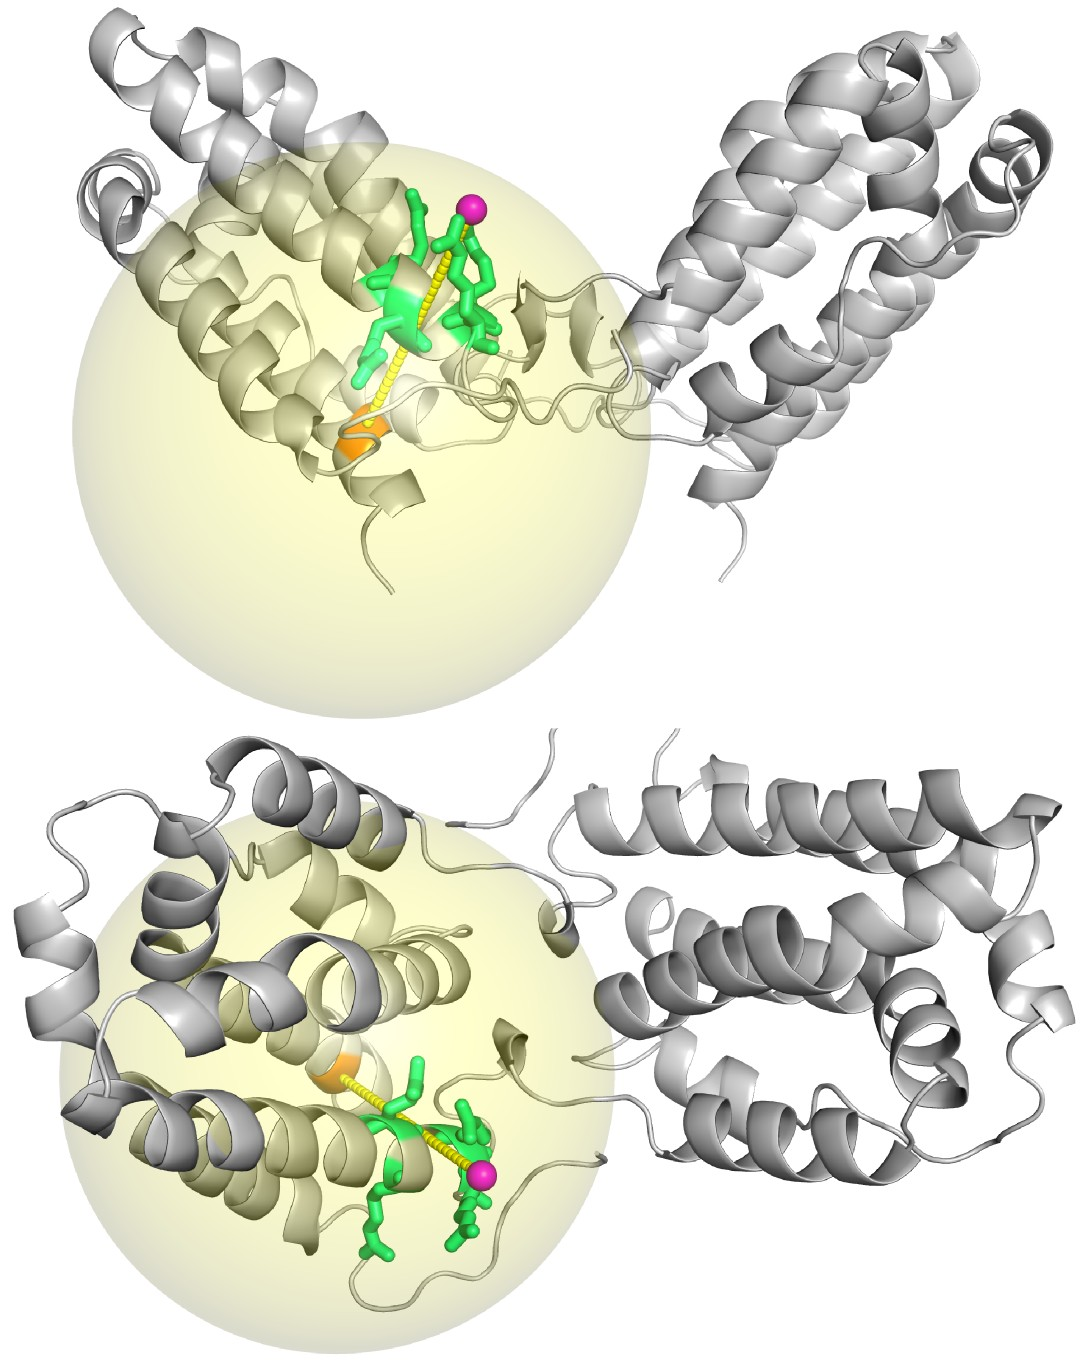
\includegraphics[width=1.0\textwidth]{gfx/dmdil10/round1_il10_ligandcenter_proteincore_sphere_top_and_side_001.jpg}
\caption[]{Geometrical DMD parameterization used for most of the DMD studies
in the first stage. The IL-10 dimer is shown in gray ribbon representation (top:
side view on the V-shape, bottom: top-down view on the V-shape). The C-alpha
atom of methionine 154 in the human interleukin-10 sequence was selected as
protein core atom (ribbon colored in orange). The focus point (small sphere
colored in magenta) was selected manually based on the putative binding region
comprised by residues R102, R104, R106, R107 (colored in green sticks). The tMD
target distance of \SI{17.7}{\angstrom} between the protein core atom and the
focus point is indicated by a thick yellow dashed line. The large transparent
yellow sphere is centered on the protein core atom and its radius is set to the
tMD target distance (after tMD, all central ligand atoms are located on that
spherical surface).}
\label{fig:dmdil10:dmd_geometry_round1}
\end{figure}

\Cref{fig:dmdil10:dmd_geometry_round1} visualizes the geometrical DMD
parameterization used for most of the DMD studies in the first stage. The manual
selection of core atom and focus point was based on the binding site prediction
made by Coulomb potential analysis (see \cref{bspred:il10}) and performed in
compliance with the guidelines formulated in \cref{dmd:lrom_preparation}. The
C-alpha atom of M154 was selected as core atom. The tMD target distance was set
to \SI{17.7}{\angstrom}, yielding a quite large spherical surface for proper
putative binding site sampling.

% If relevant, deviations from this geometrical
%setup in the first or second stage of DMD studies are described in the results
%and discussion part.

\subsubsection{DMD result consistency}

One of the first observations in this stage of DMD studies was method
consistency, i.e.\ further support for sufficient sampling and convergence of
the DMD method. \Cref{fig:dmdil10:hp_hexa_vs_tetra_clusters_position_match}
shows the overlay of two clustering results from two independently performed DMD
studies that differed only in the GAG ligand length --- one was performed with a
heparin hexasaccharide, and the other with a heparin tetrasaccharide. Ideally,
one would want DMD to return a very similar binding pose prediction in both
cases, as it is unlikely for these two GAG molecules to behave fundamentally
different. As motivated in \cref{relevance_of_clustering}, comparison of the
position of the most populated clusters in both cases is a way to (in)validate
this assumption. Note that comparison of both clusters, and with that,
comparison of both DMD studies with respect to the distribution of docking
solutions, is only possible because great care was taken of making both
clustering results comparable via the clustering parameter optimization
described in \cref{clustering_param_opt}. In both cases, the docking solution
clustering was performed with $N_{min}$ (the minimal number of clusters that
must be found) set to 1, and $M_{min}$ (the minimal number of members within
each cluster) set to 4. In both cases, the automatic clustering parameter
optimization yielded an $\epsilon$ value of \SI{2.6}{\angstrom}, i.e.\ just
about the same density of docking solutions in both clusters.

\begin{figure}
\centering
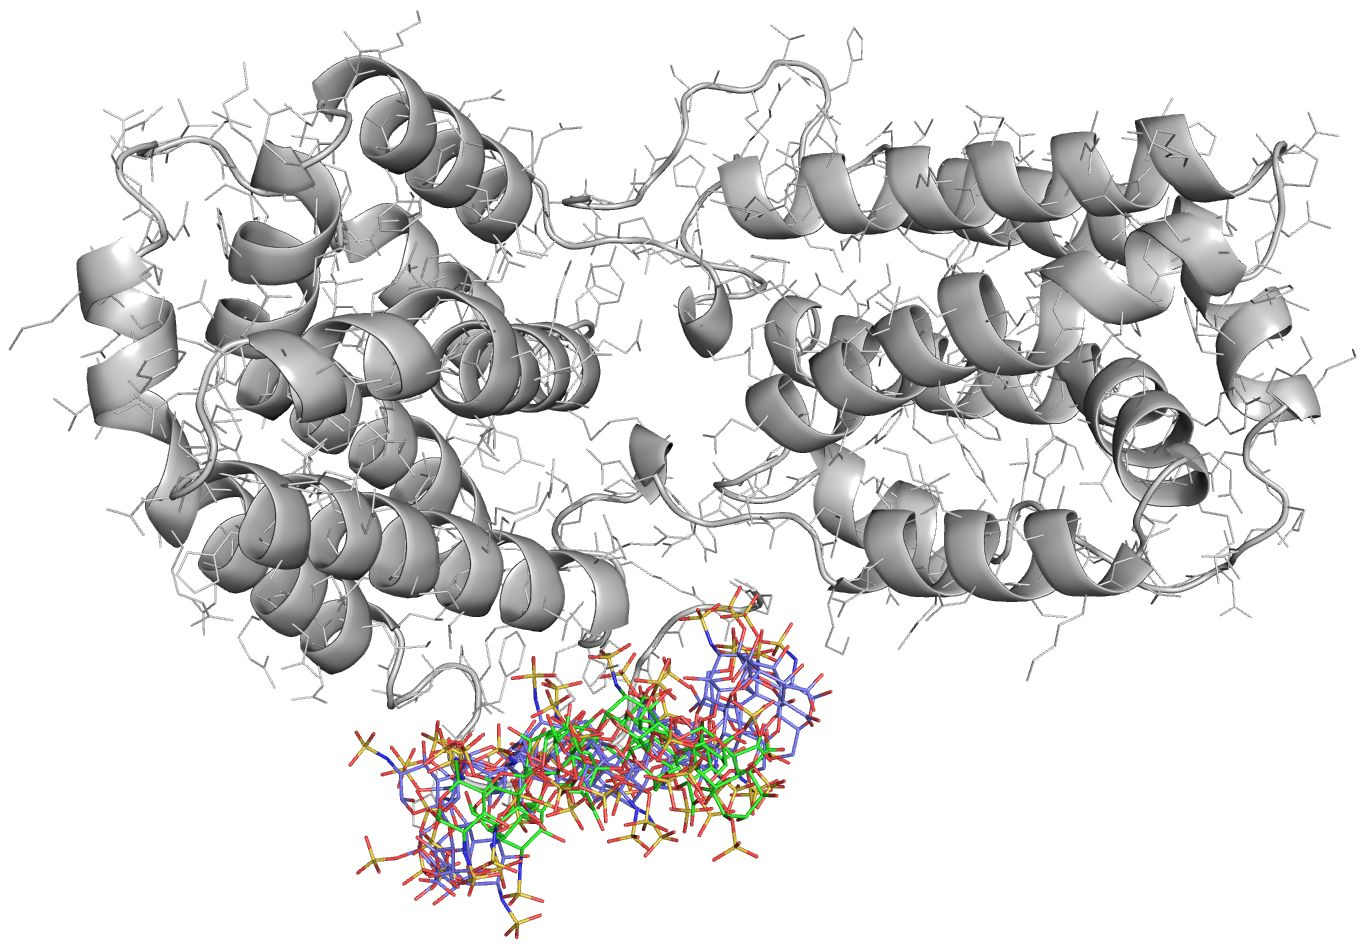
\includegraphics[width=1.0\textwidth]{gfx/dmdil10/hp_hexa_vs_tetra_clusters_position_match_cropped.jpg}
\caption[]{Consistent results among two independently conducted DMD studies.
Setup and protocol of both DMD studies differed only in the GAG ligand length,
one was performed with a heparin hexasaccharide, the other with a heparin
tetrasaccharide. The most populated cluster of docking solutions derived from
the hexasaccharide study is shown with carbon atoms in blue, and the
corresponding tetrasaccharide representation is shown with carbon atoms in
green. The IL-10 structure (PDB ID 2ILK) is shown in gray cartoon/line
representation.}
\label{fig:dmdil10:hp_hexa_vs_tetra_clusters_position_match}
\end{figure}

In essence, both clusters are positioned equivalently with respect to IL-10, and
show the same density. That is, with respect to the distribution of docking
solutions, both DMD studies returned the same result. In addition to the DMD
validation study presented in \cref{chapter:dmd}, this proves the significance
of data created by the DMD method.


\subsubsection{Impact of N-terminal residues and modest geometry changes}
%NOTE: when changing this heading, also change the "quote" in the section
% \subsubsection{Ensemble-derived single-residue energy decomposition} below.

In one of the early studies, the five N-terminal residues of IL-10 (see
\ref{dmdil10:overallmethod}) were included, and the geometrical parameterization
of DMD was varied compared to the setup described in
\ref{dmdil10:method_geom_setup_1st}: the C-alpha of M154 was kept as core atom, but
the focus point was changed slightly within the anticipated binding region,
resulting in a different orientation of the yellow axis shown in
\cref{fig:dmdil10:dmd_geometry_round1}, and in a tMD target distance of
\SI{20.5}{\angstrom} instead of \SI{17.7}{\angstrom}. The rest of the system and
protocol setup was equivalent to another DMD study (both incorporated a heparin
tetrasaccharide as ligand molecule), whose geometrical outcome is shown in
\cref{fig:dmdil10:hp_hexa_vs_tetra_clusters_position_match}. As it turned out,
the final distribution of docking solutions was not affected by the changes: the
location of the most populated clusters of both DMD studies matched. It can be
concluded that the main data obtained from a DMD study are rather insensitive
with respect to modest changes in the geometrical parameterization of DMD, and
that the presence of the five N-terminal residues does not significantly affect
the DMD binding pose prediction, i.e.\ the assumption from here on is that the
flexible part of IL-10's N-terminus can be neglected for investigating the main
mechanism of IL-10-GAG interaction.


% (the
%position of one of the clusters is shown in
%\cref{fig:dmdil10:hp_hexa_vs_tetra_clusters_position_match}).

\subsubsection{Distinction of GAG types by cluster statistics}

\begin{table}
\footnotesize
\centering
\renewcommand{\arraystretch}{1.3}
\begin{tabular}{lcrll}
\midrule
GAG type                 & cluster members & $\epsilon$ (\si{\angstrom}) & $m$ (\si{\angstrom}) & $\Delta G$ (\si{\kilo\calory\per\mol}) \\
\midrule
HP dp6                   & 4               & 2.5                         & 2.8 $\pm$ 0.7          & -45 $\pm$ 15                           \\
CS4 dp6                  & 5               & 3.2                         & 2.6 $\pm$ 0.3          & -37 $\pm$ 8                            \\
CS4 dp6 (2nd cluster) & 4               & 3.2                         & 2.4 $\pm$ 0.4          & -37 $\pm$ 14                          \\
\midrule
\end{tabular}
\caption{
Characterization of most populated clusters by single-run quantity cluster
statistics for two different DMD studies differing only in the GAG type. In one
study, a HP dp6 was used as ligand, in the other study a CS4 dp6 was used. The
HP study yielded a single prominent cluster, the CS4 study yielded two similar
clusters. $\epsilon$ is the spatial density of docking solutions according to
\cref{clustering_param_opt}. $m$ is the mobility of the ligand relative to the
receptor, as defined in \cref{dmd:dataanalysis}. Here, $\Delta G$ is the free
energy of binding estimate as provided by the MM-PBSA method
(\cref{methods:mmpbsa_mmgbsa}). The standard deviations shown are derived from
the cluster-internal variations.}
\label{tab:dmdil10:round1_different_gag_types}
\end{table}

Ideally, different behavior of different GAG types is manifests itself in the
docking solution clustering, and especially in the single-run quantities
evaluated on a per-cluster basis. The characterization of most populated
clusters for two different DMD studies differing only in the GAG type should be
discussed by means of an example. In one study, a heparin (HP) hexasaccharide
was used, in another study a chondroitin-4-sulfate (CS4) hexasaccharide was
used. The heparin study yielded a single prominent cluster, the CS4 study
yielded two almost equally populated clusters. The placement of all clusters
relative to IL-10 was similar, and the quantitative evaluation of the clusters
yielded similar results (see
\cref{tab:dmdil10:round1_different_gag_types}): among the three clusters, the
ligand movement relative to the receptor as well as the MM-PBSA free energy of
binding estimate are indistinguishable, considering the cluster-internal
fluctuations represented by the standard deviations. Just the cluster density
indicates that the docking solutions obtained for HP show more spatial
consistency than the solutions obtained for CS4.

The important conclusion to be drawn from this (and analogous observations) is
that the IL-10-GAG system does not easily allow for a binary distinction of
different GAG types via DMD with respect to their interaction \enquote{mode}.
From the DMD studies performed until here, different GAG types seem to yield
data from a continuous spectrum, showing at most quantitative differences, but
no qualitative differences in their behavior. Likewise, if there is binding
specificity of IL-10 for a certain GAG type, it remained undetectable with the
kind of data acquisition and analysis performed so far.

\subsubsection{Ensemble-derived hydrogen bonding information}

\begin{figure}
\centering
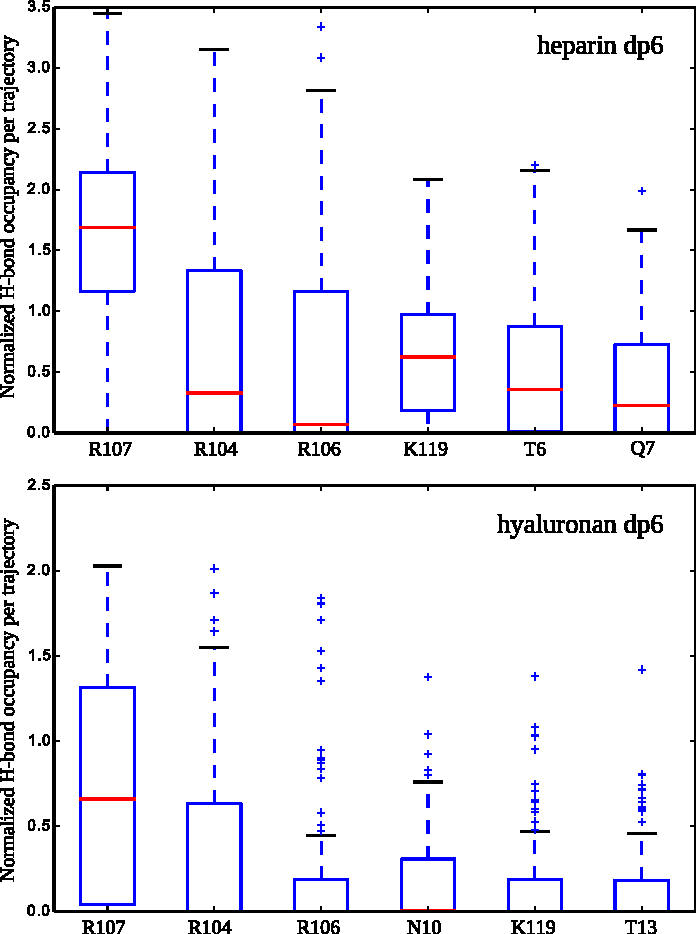
\includegraphics[width=1.0\textwidth]{gfx/dmdil10/round1_il10_hbond_hadp6_vs_hpdp6.pdf}
\caption[]{Most important residues of IL-10 for GAG-interaction, as identified
by DMD ensemble-derived hydrogen bonding information, from two independently
performed DMD studies differing \textit{only} in the GAG type (top: heparin
hexasaccharide, bottom: hyaluronan hexasaccharide). The box plot representation
is made from  $N=100$ samples per box, whereas each sample is the number of
hydrogen bond donors integrated and normalized over the data production period
of one free MD trajectory, for the residue specified in the abscissa label.
The residues are sorted by the \textit{mean} (not shown), the red bars indicate
the \textit{median} (close to zero if not visible).}
\label{fig:dmdil10:hp_hexa_vs_ha_hexa_hbond}
\end{figure}


As explained in the \enquote{extraction of ensemble properties} part of
\cref{dmd:dataanalysis}, a DMD study is able to yield reliable information
about the importance of single receptor amino acids for ligand binding, via
e.g.\ hydrogen bonding (H-bond) analysis of the MD trajectory data.
Surprisingly, all of the DMD studies performed in the first stage of studies
returned the same clear and unequivocal result --- that R107 of IL-10 plays a
major role in IL-10-GAG interaction. \Cref{fig:dmdil10:hp_hexa_vs_ha_hexa_hbond}
shows ensemble-derived H-bond information for two independently performed DMD
studies differing in the GAG type: one was performed with a HP dp6, the other
with a HA dp6. For each free MD trajectory in these two DMD studies the
normalized occupancy of H-bond donor atoms in each receptor residue was
determined, and the results were ranked by the mean normalized occupancy. All
donors within single residues were accumulated; for instance an arginine can
donate up to three hydrogens at the same time (the maximum normalized occupancy
in this case would be 3). \Cref{fig:dmdil10:hp_hexa_vs_ha_hexa_hbond} shows the
top six H-bond-donating residues for both studies, including box plot
representations of the corresponding distributions. In both cases, R107 is
ranked first by mean as well as median. In case of HP dp6, a mean R107 occupancy
of about 1.7 was measured, i.e.\ throughout the entire DMD study this residue
donated (on average) almost \textit{two} hydrogen atoms to different hydrogen
bond formations. This number alone is a strong indicator for the relevance of
this residue in protein-GAG interaction. However, the essential observation is
that R107's hydrogen bonding properties qualitatively stand out compared to the
other amino acid in IL-10: the H-bond occupancy distributions of all other
residues have their maximum near 0, and a decay towards higher occupancies,
yielding a median close to 0, in both cases shown (HP dp6 and HA dp6). The
occupancy distribution of R107, however, has a median clearly far from 0. In
case of HP dp6, the distribution has its global maximum at about 1.5. It can be
concluded that most of the molecular surface of R107 is solvent-exposed, and
significantly more accessible for interaction with functional groups of GAGs
than the other residues.

Hyaluronan has significantly less functional groups (carboxyls and sulfates)
available that might act as H-bond acceptors than heparin. Quantitatively, this
difference is clearly reflected in the mean value of the H-bond occupancy
distributions, with about 1.7 for HP dp6 and about 0.7 measured for HA dp6. For
all different GAG types and lengths investigated in the first stage of IL-10-GAG
DMD studies (CS4 dp4, CS6 dp4, HA dp4, HP dp4, figures not shown for all GAG
types), R107 showed distinct behavior by the quantitative and qualitative
criteria described in the paragraph above. A clear conclusion is that R107
significantly stands out compared to all other residues and supposedly plays a
particularly important role in IL-10- GAG recognition.

\subsubsection{Ensemble-derived single-residue energy decomposition}

\begin{figure}
\centering
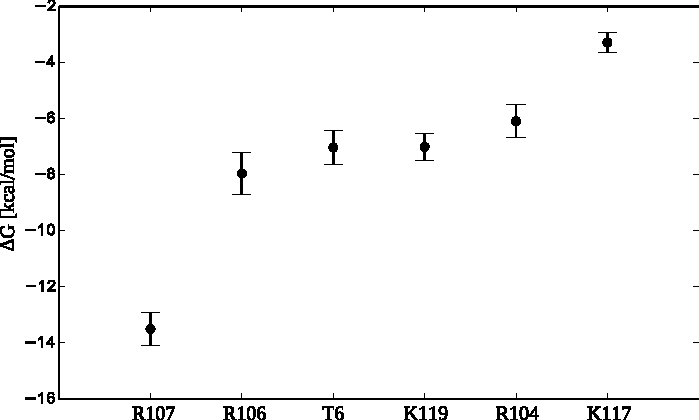
\includegraphics[width=0.97\textwidth]{gfx/dmdil10/round1_il10_SRED_hpdp6.pdf}
\caption[]{Merged single-residue energy decomposition (SRED) data from a
DMD study with a HP dp6 ligand. The DMD study was comprised of 200 runs. The
SRED data of the top \SI{40}{\percent} of the DMD runs ranked by MM-PBSA
$\Delta G$ were merged into the data points shown. The error bars represent the
standard error of the mean.}
\label{fig:dmdil10:SRED_hpdp6}
\end{figure}

I have observed the ensemble-merged MM-GBSA single-residue energy decomposition
(SRED, as explained in the \enquote{extraction of ensemble properties} part of
\cref{dmd:dataanalysis}) data to yield results generally consistent with those
of the hydrogen bonding analysis. Most importantly, the SRED data also points
out the importance of R107 for IL-10-GAG recognition.
\Cref{fig:dmdil10:SRED_hpdp6} shows the six top-ranked IL-10 residues according
to SRED performed on a DMD study with a HP dp6. In this case, the DMD study was
comprised of $N=200$ DMD runs, and the SRED data of the top \SI{40}{\percent} of
the DMD runs according to the MM-PBSA free energy of binding estimate has been
merged, yielding 80 DMD runs contributing to the data shown. The error bars
represent the standard error of the mean, and one can conclude that ---
considering the statistical error --- the residues on ranks two to five are not
distinguishable, ranging in the interval between \SI{-6}{\kilo\calory\per\mol}
and \SI{-8}{\kilo\calory\per\mol}. R107, however, has a special role, with a
significantly stronger mean interaction energy of \SI{-13.5 +-
0.5}{\kilo\calory\per\mol}. Note that the absolute values of these energies as
well as the inter-residue energy distance are not meaningful. The relative
distances, however, yield resilient information. As in case of hydrogen bonding
data, those DMD studies in the first stage of studies differing from the
above-described setup in GAG type and length also revealed R107 as having the
strongest interaction with the GAG, leaving all other residues far behind (data
not shown).

Further insights were derived from the SRED data obtained from the IL-10-GAG DMD
studies in the first stage. For instance, the DMD study with a HA dp6 used as
ligand led to the same qualitative SRED results as discussed in the paragraph
above, in the sense that R107 stood out. However, the corresponding mean
interaction energy was determined as \SI{-3.8 +-0.3}{\kilo\calory\per\mol},
which is about \SI{70}{\percent} weaker than in case of the HP dp6 study.
Qualitatively this drop is expected as of the fewer sulfate groups in HA
compared to HP. Also, the observation is in compliance with the hydrogen bonding
data discussed in the previous section, where we observed a drop of about
\SI{60}{\percent} in the R107 hydrogen bond occupancy when changing from heparin
to hyaluronic acid.

In general, it can be concluded that both, SRED and hydrogen bonding analysis
are able to identify R107 as especially important, whereas the hydrogen bonding
analysis is computationally less complex than SRED. Furthermore, both types of
analyses can quantitatively express the effect of a drop in the number of
sulfate groups per repeating GAG unit. Another interesting observation made is
that inclusion of IL-10's N-terminus does not significantly influence the
outcome of SRED as well as hydrogen bonding data, in line with the conclusions
drawn in the \enquote{Impact of N-terminal residues and modest geometry changes}
part above.



\subsubsection{Mutating IL-10's arginine 107 to alanine}

\begin{figure}
\centering
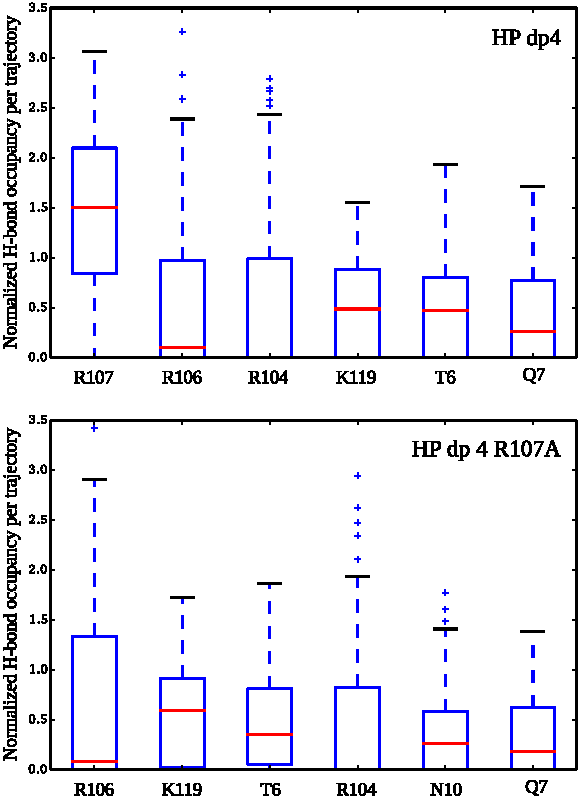
\includegraphics[width=1.0\textwidth]{gfx/dmdil10/first_stage_Hbonding_hp_dp4_R107A_vs_unmutated.pdf}
\caption[]{Most important residues of IL-10 for GAG-interaction, as identified
by ensemble-derived hydrogen bonding information from two independently
performed DMD studies using a HP dp4 ligand, and differing only in the IL-10
sequence at position 107. Top: canonical human IL-10 sequence. Bottom: R107A
mutation. The box plot representation is made from $N=100$ samples per box,
whereas each sample is the number of hydrogen bond donors integrated and
normalized over the data production period of one free MD trajectory, for the
residue specified in the abscissa label. The residues are sorted by the
\textit{mean} (not shown), the red bars indicate the \textit{median} (close to
zero if not visible).}
\label{fig:dmdil10:hpdp4_normal_vs_R107A}
\end{figure}

Up to here, various observations have been made, independently suggesting that
R107 has an important role in IL-10-GAG interaction. For further characterizing
the impact of this residue, a DMD study was performed with an R107A mutation of
the IL-10 sequence while keeping all other parameters equivalent to another
study performed before, both using a HP dp4 molecule as ligand. The most
concrete observation from this comparison stems from hydrogen bonding and SRED
analysis. No other amino acid residue was able to compensate the loss of the
polar and hydrogen bonding properties of R107, not even its neighboring
arginines: with the R107A mutation, the hydrogen bond occupancy of the
non-mutated residues did almost not change, as shown in
\cref{fig:dmdil10:hpdp4_normal_vs_R107A}. The box plot representations of the
hydrogen bonding occupancy of R104, R106, and K119 indicate similar behavior in
both studies. Particularly, the box plot representation of the hydrogen bonding
occupancy of R107 in the non-mutated IL-10 finds no resemblance in the DMD study
with the mutant protein. The SRED analysis for the non-mutated system yielded an
interaction energy of
\SI{-13.5 +- 0.8}{\kilo\calory\per\mol} for R107, leaving all other residues far
behind, and R106 was assigned an energy of \SI{-5.5 +-
0.8}{\kilo\calory\per\mol}. In contrast, the SRED analysis for the mutated
system ranked R106 first, with an interaction energy of \SI{-8 +-
1.0}{\kilo\calory\per\mol}, indicating a weak compensation effect, in the sense
that R106 becomes slightly more important for GAG-binding in case of the R107A
mutation. However, also the SRED analysis reveals that the qualitative nature of
the interaction between R107 and the tested GAG molecules can not be reproduced
by any other amino acid in that region, supporting the picture in which R107
takes a \textit{unique} role for IL-10-GAG interaction. All in all, these
observations further corroborate the importance of R107 for IL-10-GAG
interaction.


\subsection{2nd stage of DMD studies}


\subsubsection{Optimized DMD parameterization}
\label{dmdil10:method_setup_2nd}

In the second stage of IL-10-GAG DMD studies, the geometrical parameterization
was chosen based on the docking solution clustering results obtained in the
first stage. There, the most populated clusters of docking solutions were mostly
located in the same place, positioned very similar to the clusters shown in
\cref{fig:dmdil10:hp_hexa_vs_tetra_clusters_position_match}.  Following the
paradigm of the iterative method for obtaining convergence, the DMD focus point
was aligned towards this agglomeration of DMD docking solutions, in order to
further focus the sampling onto that region: the new focus point was set onto
the central atom of a representative docking solution from above-mentioned
clusters. The C-alpha atom of M154 was kept as core atom, yielding a tMD target
distance of \SI{20.5}{\angstrom}.

An optimization implemented in the second stage of DMD studies was the reduction
of the target displacement length for the LROM setup. It was shortened from
\SI{30}{\angstrom} to \SI{25}{\angstrom}, effectively decreasing the system size
and therefore the computational effort for performing the tMD simulations.
Furthermore, the tMD simulation time was decreased from \SI{4}{\nano\second} to
\SI{3}{\nano\second}. Overall, 98 DMD runs were completed for CS4 dp6, 200 runs
for CS6 dp6, 198 runs for HA dp4, 278 runs for HA dp6, 194 runs for HP dp4, and
298 runs for HP dp6.


\subsubsection{SRED results}


\begin{figure}
\centering
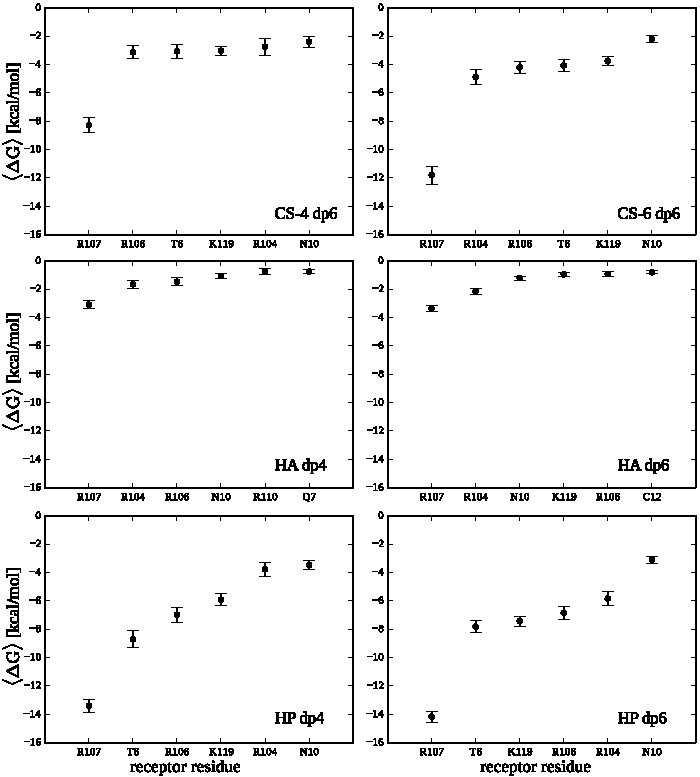
\includegraphics[width=1.0\textwidth]{gfx/dmdil10/second_stage_all_SREDs_05.pdf}
\caption[]{
Merged single-residue energy decomposition (SRED) data for six independently
performed DMD studies differing only in the type of ligand, as indicated in the
right bottom corner of each plot. The data shown stems from 98 DMD runs
completed for CS4 dp6, 200 runs for CS6 dp6, 198 runs for HA dp4, 278 runs for
HA dp6, 194 runs for HP dp4, and 298 runs for HP dp6. The SRED data of the top
\SI{40}{\percent} of the DMD runs ranked by MM-PBSA $\Delta G$ were merged into
the data points shown. The error bars represent the standard error of the mean.
}
\label{fig:dmdil10:2nd_stage_all_SREDs}
\end{figure}

\Cref{fig:dmdil10:2nd_stage_all_SREDs} shows all SRED results obtained from the
second stage of DMD studies. Again, R107 ranks first in all studies.
Qualitatively, for all GAG types containing sulfate groups (not HA), there is a
clear separation between R107 and the residues ranked second or worse. Ranks two
to six are not well-resolved in all cases, considering the error bars which
represent the statistical error of the method. Quantitatively, the energetic
contribution of single amino acid residues is shown to be much larger for
sulfated GAGs than for HA. In these lines, the observations obtained from the
first stage of DMD studies are reproduced.

Another observation is that for HP as well as for HA, which have both been
analyzed as dp4 and dp6 variants, there is no significant difference in the SRED
result depending on the length of the GAG. That is, at least within the scope of
the methodology used here, tetra- and hexasaccharides are identified to show
qualitatively the same behavior.

An important observation is that the set of the top six residues obtained from
SRED in the second stage of studies is the same for all sulfated GAG types
(i.e.\ for HP, CS4 and CS6): R107, R106, R104, K119, T6, N10. This is another
evidence for the convergence of the DMD method and its subsequent data analysis.
Additionally, this expresses that the resides ranked two to six --- while their
internal ranking might be unclear --- have not been identified as important by
coincidence (noise), but arguably actually contribute more to GAG binding than
other residues not listed in the top six. When the set of top six residues
identified for the sulfated GAG types is compared to the binding region
prediction made in \cref{chapter:bspred}, one notes that R102 does not appear in
any of the top six rankings. That R102 does not appear here might be due to the
localized nature of the DMD method, and it could be that the location bias
introduced via the geometrical DMD parameterization does not allow R102 to be
properly sampled by the ligand. However, since R102 is spatially so close to
R106 and R107, I tend to conclude that R102 actually \textit{is} less important
for GAG binding than initially assumed just based on the Coulomb potential
distribution. A notable observation in this context is the importance of T6,
which might actually be an artifact: in all second stage DMD studies, T6 is the
N-terminal residue of IL-10, and therefore it is quite accessible for the
ligand, whereas in reality it is not the terminus.

Regarding the DMD method itself, one can conclude that the reduction of the
target displacement length to \SI{25}{\angstrom} and the reduction of pulling
process simulation time to \SI{3}{\nano\second} did not lead to observable
caveats --- in fact, the results described so far from the second stage of DMD
studies are in compliance with those DMD results obtained in the first stage of
studies.


\subsubsection{Docking solution clustering}


\begin{figure}
\centering
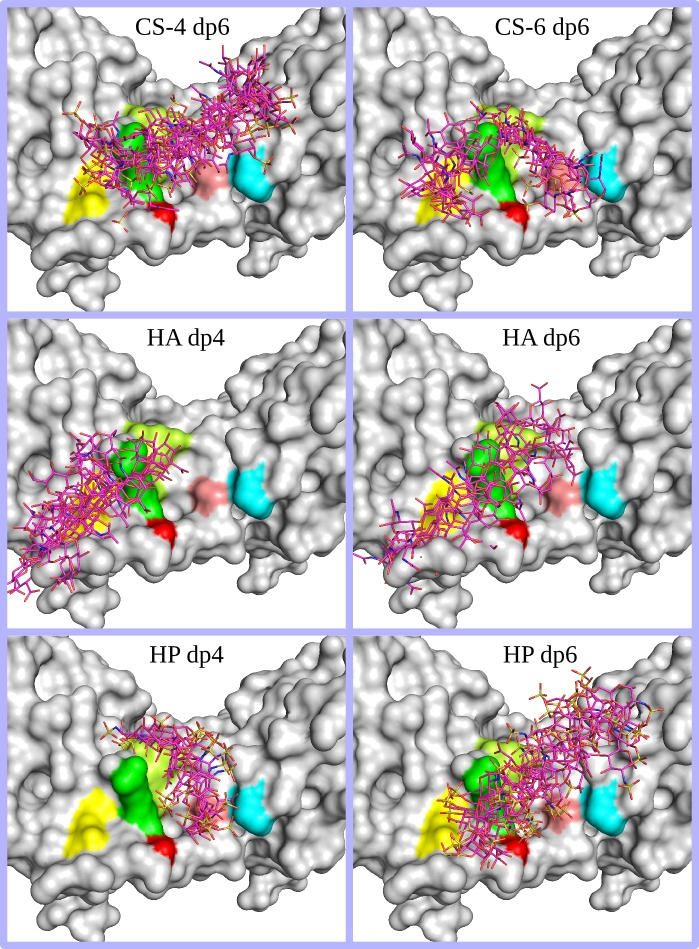
\includegraphics[width=1.0\textwidth]{gfx/dmdil10/2ndstage_allclusters_04.jpg}
\caption[]{
Most populated docking solution clusters of all second stage DMD studies,
obtained with a consistent approach. The studies differ only in the GAG type and
length (as defined in the panel headings). The GAG structures within each
cluster are shown with carbon atoms in magenta. The IL-10 structure (PDB ID
2ILK) is shown in gray surface representation. The surface of the reproducibly
obtained top six set of residues according to the ensemble-derived SRED analysis
is colorized: R107 in green, R106 in light green, R104 in yellow, K119 in
cyan, N10 in red, and T6 in light red.}
\label{fig:dmdil10:2nd_stage_all_clusters}
\end{figure}



\Cref{fig:dmdil10:2nd_stage_all_clusters} shows the most populated docking
solution clusters for all second stage DMD studies. In all cases, the clustering
was performed with $N_{min}$ (the minimal number of clusters that must be found)
set to 1, and $M_{min}$ (the minimal number of members within each cluster) set
to 5, i.e.\ the clustering results are comparable (see \cref{chapter:clustering}
for details). There are a couple of important observations to be made from these
data. First of all, there are two principally different GAG binding orientations
found, both heavily involving R107. From the point of view shown in
\cref{fig:dmdil10:2nd_stage_all_clusters}, one principal binding pose is
oriented from the bottom left to the upper right, with the GAG being placed in a
IL-10 surface groove below R107. This is true for CS4 dp4, for both HA
scenarios, and for HP dp6. A second qualitatively different pose is oriented
from the top left to the bottom right, with the GAG placed above R107, and
squeezed between R107 and K119 (shown in green and cyan in the figure,
respectively). This is true for the HP dp4 scenario. The structures in the CS6
dp6 cluster are bent in a way that they can be considered a combination of both
principal binding poses. \Cref{fig:dmdil10:2nd_stage_principal_poses} visualizes
both principally different poses schematically.

\begin{figure}
\centering
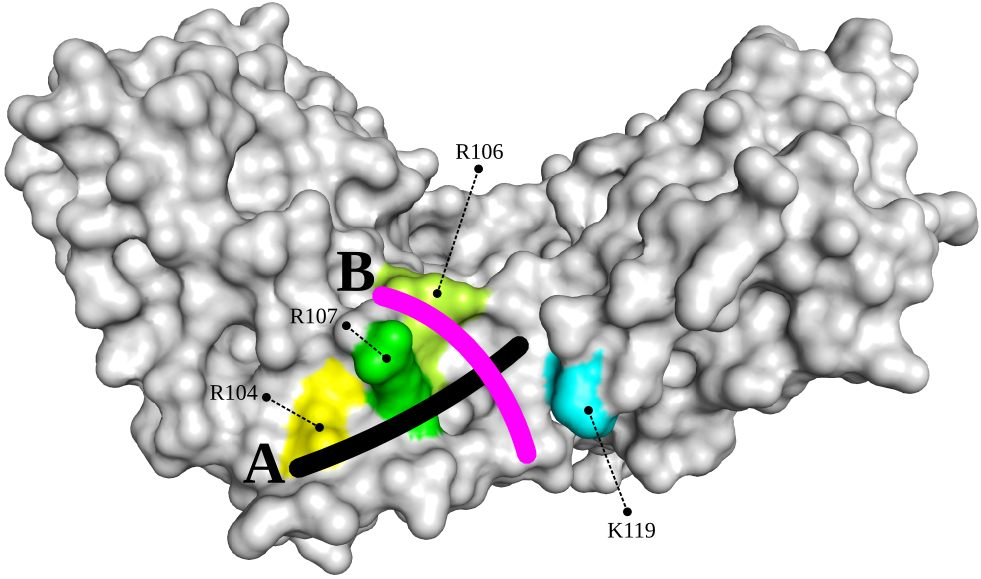
\includegraphics[width=1.0\textwidth]{gfx/dmdil10/principal_poses_06.jpg}
\caption[]{
Schematic visualization of two principally different GAG binding poses observed
via docking ensemble clustering of all second stage DMD studies. Pose A
(indicated in black) has the GAG placed in a IL-10 surface groove right
\enquote{below} R107 (from the point of view shown here). Pose B (indicated in
magenta) has the GAG placed above R107 and within the groove between R107 and
K119. The IL-10 structure (PDB ID 2ILK) is shown in gray surface representation.
The four positively charged residues being most important for GAG binding
(according to ensemble-derived SRED analysis) are labeled and their surface is
colorized.}
\label{fig:dmdil10:2nd_stage_principal_poses}
\end{figure}

It is notable that there actually is a qualitative difference for the cluster
poses obtained for HP dp4 and HP dp6. This is not supported by the SRED data
described in the section before, where it was found that HP tetra- and
hexasaccharides show qualitatively the same behavior. This is not \textit{per
se} a contradiction, since the SRED data represent a large ensemble of docking
solutions, while clustering explicitly selects a small fraction of the ensemble,
under the assumption that this fraction represents the most probable state.
However, since the clustering method introduces assumptions and approximations
on top of the DMD approach --- which increases the overall uncertainty --- the
SRED ensemble data is more reliable than the clustering result. Therefore, as of
a lack of support from the SRED data, none of both principal binding
orientations discussed above must be excluded for both, HP dp4 and dp6.

Looking at the structure ensembles shown in
\cref{fig:dmdil10:2nd_stage_all_clusters} it makes sense that K119 has been
identified (via SRED) as being a strong contributor to GAG binding: the groove
between R107 and K119 could serve as a trap, potentially anchoring a GAG from
two sides simultaneously, with a positively charged amino acid residue on both
sides. The groove is just wide enough for e.g.\ heparin, as can be seen in the
HP dp4 panel of \cref{fig:dmdil10:2nd_stage_all_clusters}. The clustering data
can be used for characterizing the impact of this groove on GAG behavior: the HP
dp4 cluster (which is located in mentioned groove) shows the highest structural
consistency among all clusters shown in
\cref{fig:dmdil10:2nd_stage_all_clusters}. The similarity among the structures
in this cluster has been quantified with $\epsilon = \SI{2.2}{\angstrom}$ (this
value actually encodes the \enquote{density-reachabiltiy}, and the smaller the
value, the larger the similarity; see \cref{chapter:clustering} for details).
This structural consistency is significantly larger than in the other cases (HP
dp6: $\epsilon = \SI{2.6}{\angstrom}$, HA dp4: $\epsilon = \SI{3.0}{\angstrom}$,
HA dp6: $\epsilon = \SI{2.6}{\angstrom}$, CS4 dp6: $\epsilon =
\SI{3.4}{\angstrom}$, CS6 dp6: $\epsilon = \SI{2.7}{\angstrom}$). Presumably,
the reason for this comparably large structural consistency is that heparin
tightly fits into this groove, with less conformational freedom when compared to
the other binding modes shown in \cref{fig:dmdil10:2nd_stage_all_clusters}.


\subsection{Conclusions}

Various DMD studies involving IL-10 and different GAGs have been performed. An
important intermediate result of the corresponding data analysis is that one
amino acid residue, R107 (in the hIL-10 sequence, conserved in mouse),
significantly stands out compared to all other residues and supposedly plays a
particularly important role in IL-10-GAG recognition. This conclusion is based
on different reliable types of data, including ensemble- and time-averaged
hydrogen bonding analysis and single-residue energy decomposition applied to
molecular dynamics data collected on the microsecond time scale.

It is this kind of data that also revealed that R102 might be less important for
GAG binding than initially assumed based on the binding region prediction
discussed in \cref{chapter:bspred}. Furthermore, K119 --- which was left
undiscussed in \cref{chapter:bspred} --- potentially plays an important role, as
it might cooperate with R107 in trapping a GAG from two sides simultaneously.
This structural model of IL-10-GAG interaction is supported by clustering data
that led to the observation of two principally different GAG binding poses in
the region of interest, both heavily involving R107.

The IL-10-GAG DMD studies led to a further consolidation of the DMD method
compared to its initial presentation in \cite{dmd_samsonov_gehrcke_2014}.
Specialized hardware was established and a software framework for managing DMD
studies was developed, both for performing DMD studies efficiently and on a
large scale. Furthermore, the protocol details of the method were fine-tuned,
and further evidence was obtained showing that DMD yields well-converged --- and
therefore reliable --- data.

\chapter{Evaluation of NMR data for examining IL-10-GAG interaction}

The combination of both, \textit{in silico} methods and nuclear magnetic
resonance (NMR) data, often leads to an improved understanding of the system
under investigation, compared to the insights obtained with either approach
individually. This is especially true for protein-GAG systems, where \textit{in
silico} simulations are usually performed based on NMR data in order to obtain a
structural model with larger spatial resolution than achievable from NMR data
alone. The principal complementarity of NMR and \textit{in silico} methods with
respect to protein-GAG systems has been demonstrated and published before, for
instance in \cite{pichert_characterization_2012, sost_heparin_2009,
nieto_conf_selection_heparin_2011}.

In an ongoing effort, G. Künze from Prof. D. Huster's laboratory at the
Universität Leipzig investigates the IL-10-GAG system with NMR methods. In this
chapter, I describe how I post-processed his nuclear Overhauser effect
spectroscopy data in order to derive heparin tetrasaccharide structure models
for the free state (without IL-10 in solution) and bound state (with IL-10 in
solution) and discuss the implications of the corresponding results. This work
is part of our collaborative publication titled \enquote{NMR characterization of
the binding properties and conformation of glycosaminoglycans interacting with
interleukin-10} in the \textit{Glycobiology} journal \cite{kuenze_gehrcke_2014}.
Additionally, in this chapter I summarize further insights derived from G.
Künze's data and discuss them in the context of the conclusions drawn in this
thesis so far.

%The combination of insights gained via \textit{in silico} methods and
%experimentally obtained data has led to an improved understanding of the
%molecular recognition principles governing the IL-10-GAG system. This chapter
%presents the studies and outcomes of this collaborative effort.

\section{HP dp4 structure in dependence of IL-10 presence}

\subsection{Background: NOESY for inter-atomic distance determination}

In essence, the spins of atomic nuclei that are spatially close to each other
(closer than about \SI{5}{\angstrom}) may undergo a significant dipole-dipole
interaction, leading to the measurable effect of nuclear spin polarization
transfer from one nuclear spin population to another. In other words, after
excitation, two dipolar-coupled spins do not relax independently, which is
called the nuclear Overhauser effect (NOE). In two-dimensional nuclear
Overhauser effect spectroscopy (NOESY) experiments, this correlation effect
manifests itself in form of off-diagonal resonance peaks. In first order
approximation (or \enquote{isolated two-spin approximation}), the intensity of
such a so-called cross peak is proportional to the cross-relaxation rate
constant for the two-spin system. Due to the dipolar nature of the spin-spin
interaction, this rate constant is proportional to the inverse sixth power of
the distance between the two spins \cite{neuhaus2000_noe}. Likewise, the main
usage of the nuclear Overhauser effect in NMR spectroscopy for biological
questions is the detection of distances between pairs of protons. Eventually and
under ideal conditions, NOESY can be used for collecting sufficient geometrical
information about a certain molecule for determining a three-dimensional
structure of that molecule. In practice, depending on the environmental
conditions and on the type of molecules investigated, there are various sources
of error that can prevent NOE cross peaks from building up, or that
significantly invalidate the assumption of a linear dependence between the peak
intensity and the relaxation rate constant \cite{palmer_online_nmr_relaxation},
affecting at least the spatial resolution of the data, or even the ability to
obtain meaningful NOE data at all.


\subsection{Methods}

Our collaborator G. Künze performed NOESY experiments for measuring
heparin-internal hydrogen-hydrogen distances for a heparin tetrasaccharide (HP
dp4) in solution, in two different conditions: once with presence of \hl{murine}
IL-10, and once without presence of IL-10. Ideally, the geometry information in
this data can be used for creating HP dp4 structure models for what we call the
\enquote{bound} and \enquote{unbound} state (with and without IL-10,
respectively).

The creation structure models from the NOESY-derived distance data is an
optimization problem with the goal of finding the heparin structure fulfilling
the experimentally obtained distance constraints as good as possible. We have
approached this optimization problem with simulated annealing molecular dynamics
simulations.

The following parts skip details regarding the NMR experiments and rather
describe and discuss the evaluation of distance data. For particular method
details and further discussion we kindly refer the reader to the manuscript
corresponding to this study which, \hl{at the time of writing this thesis, has
been submitted for publication.}


HP dp4-internal ${}^1$H-${}^1$H distances were calculated
from experimentally obtained NOE intensities assuming a $1/r^6$ distance
dependence between interacting protons. Calibration was based on the H2-H4 and
H3-H5 proton pairs of the GlcNS,6S ring with a known distance of
\SI{2.55}{\angstrom} in the ${}^4$C${}_1$ chair conformation. A tolerance
interval of $\pm \SI{0.3}{\angstrom}$, $\pm \SI{0.6}{\angstrom}$ and $\pm
\SI{1.0}{\angstrom}$ was used for measured distances $< \SI{2.0}{\angstrom}$,
between \num{2.0} and $\SI{4.0}{\angstrom}$, and $> \SI{4.0}{\angstrom}$,
respectively.

The experimentally obtained  distance restraints were used for GAG structure
determination using MD simulations employing Amber 12 \cite{case_amber_12}. Atom
types of the GLYCAM 06g force field \cite{kirschner_glycam06:_2008} were used to
build the heparin tetrasaccharide $\Delta$UA,2S-GlcNS,6S-IdoA,2S-GlcNS,6S,
referred to as rings A, B, C, D, respectively. Sulfate partial charges were
obtained from RESP calculations for methylsulfate at the 6-31(d)G level of
theory. The first structure optimization stage was a simulated annealing
protocol using a simple implicit solvent model with a 1/r distance dependency of
the dielectric constant. The protocol contained the following steps: \textit{i)}
steepest descent and conjugate gradient minimization without restraints,
\textit{ii)} 100 ps MD with tight coupling to a \SI{600}{\kelvin} heat bath and
gradual activation of NMR distance restraints, \textit{iii)}
\SI{300}{\pico\second} MD with restraints, gradual temperature change from
\SI{600}{\kelvin} to \SI{10}{\kelvin}, and normal coupling to heat bath,
\textit{iv)} short MD with gradual cooling to \SI{0}{\kelvin} and tight coupling
to heat bath. The MD time step for this protocol was set to
\SI{1}{\femto\second}. The second optimization stage was performed with periodic
boundary conditions in TIP3P explicit solvent (with at least \SI{8}{\angstrom}
from all solute atoms to the box boundary), with Na+ ions for system
neutralization, using SHAKE, and with an MD time step of \SI{2}{\femto\second}.
The following steps were performed: \textit{i)} solvent minimization with
constrained solute, \textit{ii)} \SI{20}{\pico\second} heat up MD to
\SI{300}{\kelvin} in NVT ensemble with strong positional restraints on solute
atoms, \textit{iii)} \SI{200}{\pico\second} equilibration MD in NPT with weak
positional restraints on solute atoms and NMR distance restraints, \textit{iv)}
\SI{200}{\pico\second} MD in NPT with NMR distance restraints and a gradual
cooling to \SI{250}{\kelvin}, \textit{v)} \SI{400}{\pico\second} MD in NPT with
NMR distance restraints and a gradual cooling to \SI{0}{\kelvin}. Beyond the
tolerance interval, each NMR distance restraint was implemented with a harmonic
potential with a force constant of \SI{20}{\kilo\calory\per\mole\per\angstrom}.
Since GLYCAM does not contain proper parameters for 4,5-unsaturated uronic acid,
NOE signals involving hydrogens of ring A other than H1 were not applied as
restraints in the simulations.The two stages of structure optimization were
repeated 100 times in independent simulations with different random seeds. All
optimized structures were aligned to each other. Structure alignment was based
on all ring atoms of rings B, C, D, and all glycosidic linkage oxygens. The root
mean square distance (RMSD) among these atoms was calculated to obtain the
structural distance between any two given structures. The structural diversity
within the ensemble was quantified by calculating the mean pairwise structural
distance among all aligned structures. The structure having the lowest mean
structural distance to all other structures in the ensemble was selected as the
representative of the ensemble.

For structure characterization, the distribution of various dihedral angles was
evaluated for all structures in an ensemble. For analyzing the GAG backbone
structure, we measured the glycosidic linkage torsional angles Φ, defined by
atoms H1-C1-O4-C4, and Ψ, defined by C1-O4-C4-H4, both in direction from the
non-reducing end to the reducing end of the GAG. Additionally, we measured the
orientation of sulfate side-chains via the dihedral angles H2-C2-O-S for
2-O-sulfates, H2-C2-N-H for 2-N-sulfates, and O5-C5-C6-O6 for 6-O-sulfates.

\subsection{Results and discussion}

\begin{figure}
\centering
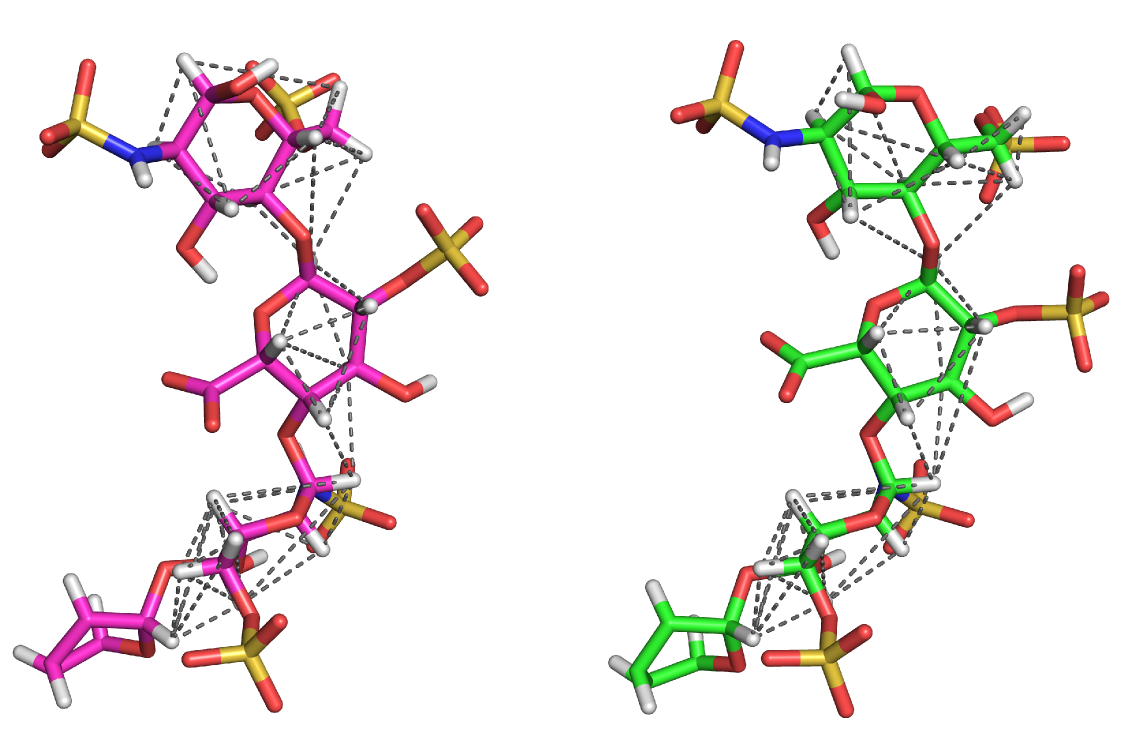
\includegraphics[width=0.7\textwidth]{gfx/nmr/two_cases_dashed_lines_distances.png}
\caption[]{
Heparin tetrasaccharide-internal H-H distance restraints applied during
simulated annealing MD simulations. Each dashed line corresponds to one NMR
distance restraint. In the unbound case (left, carbon in magenta), 42
restraints were applied. In the bound case (right, carbon in green), 41
restraints were used. Functional groups of ring A are not shown for clarity.
Atoms are color-coded with red, blue, yellow, gray corresponding to oxygen,
nitrogen, sulfur, and hydrogen, respectively.
}
\label{fig:nmr:hp_dashed_lines_distances}
\end{figure}

\begin{figure}
\centering
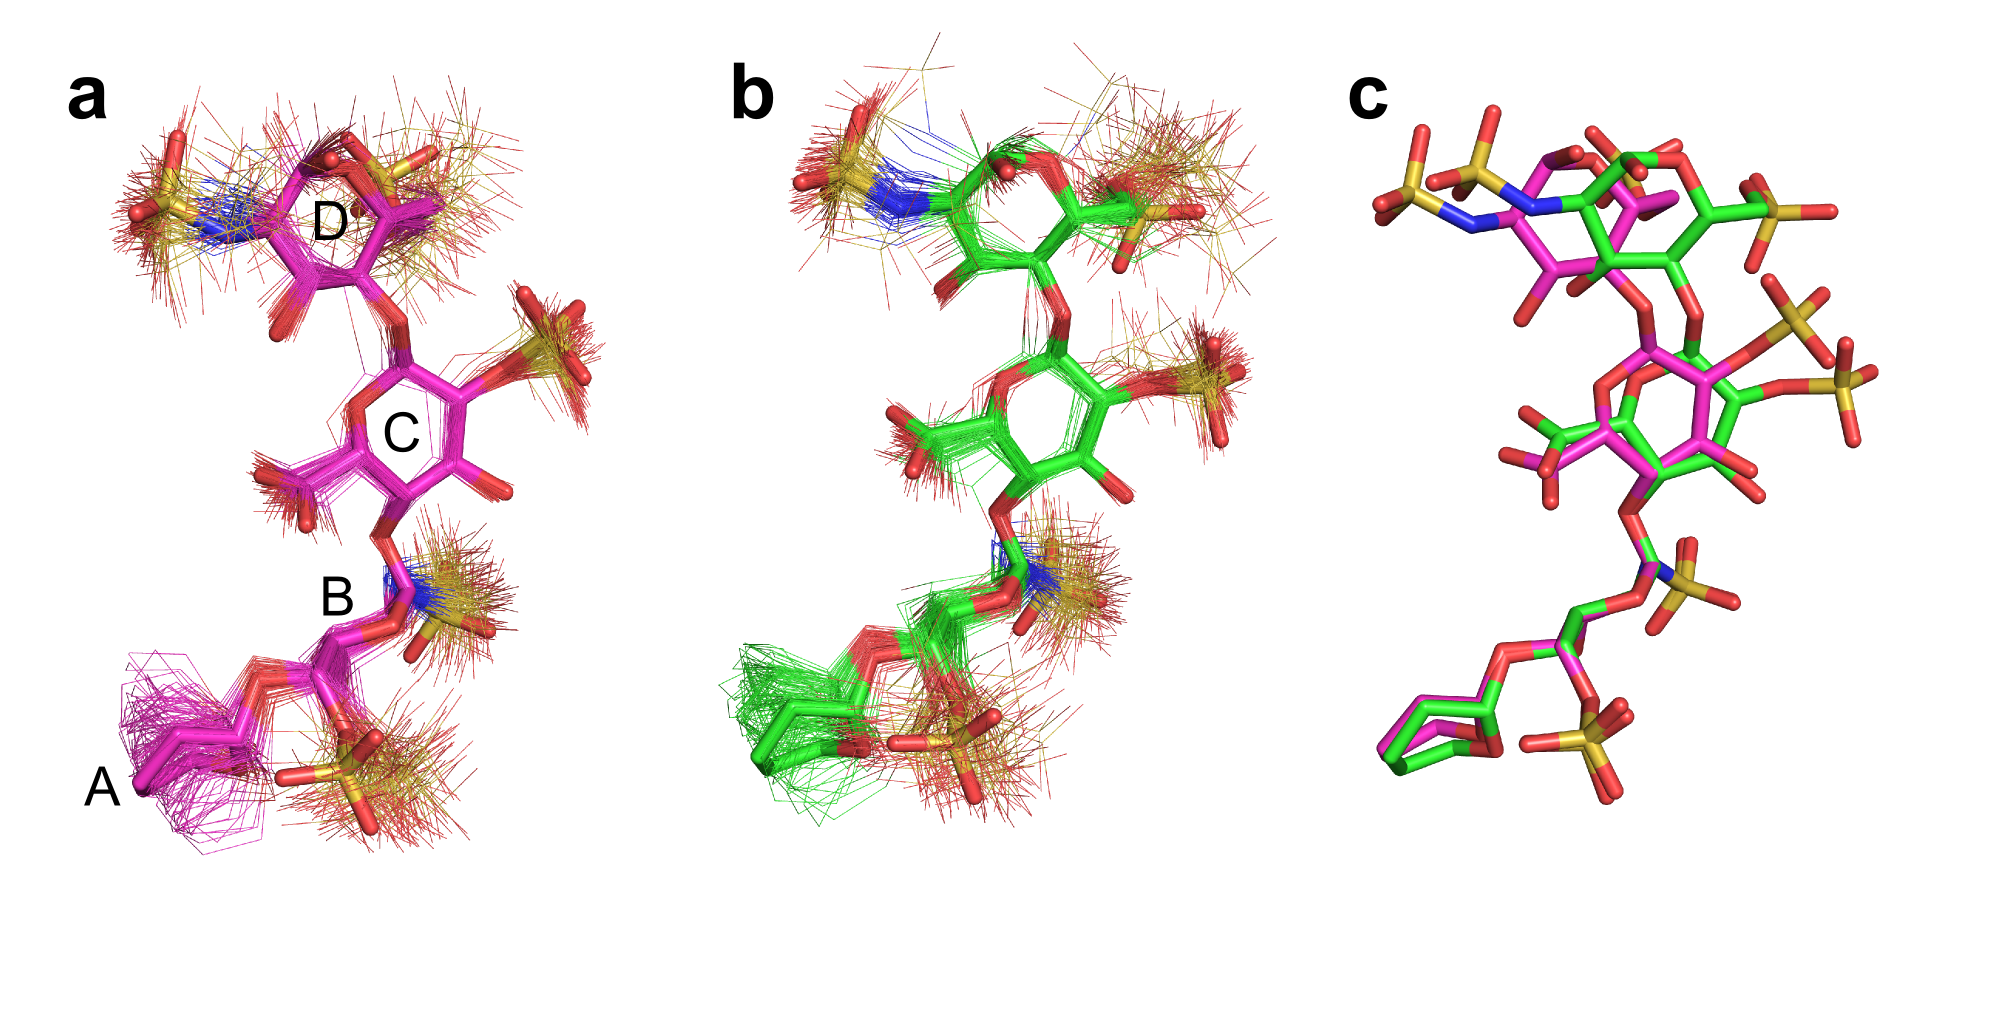
\includegraphics[width=\textwidth]{gfx/nmr/Figure_07_bound_vs_free_three_panels_05.png}
\caption[]{
Heparin structure models obtained from NOE data and simulated annealing
simulations. (a) structure model ensemble for the unbound case (ring identifiers
in capital letters). (b) structure model ensemble for the bound case. (c) the
representative structure for both, the unbound (carbons in magenta) and bound
(carbons in green) ensembles, aligned on ring B. The ensemble representatives
are shown in thick sticks. Functional groups of ring A and hydrogens are not
shown for clarity. Atoms are colored by type (oxygen: red, nitrogen: blue,
sulfur: yellow).
}
\label{fig:nmr:hp_ensembles_representatives}
\end{figure}

We created structural models of heparin based on internal NOE data by performing
simulated annealing MD simulations including hydrogen pair distance restraints
for the unbound heparin tetrasaccharide and for heparin in the presence of
IL-10. In the unbound case, 42 H-H distance restraints were applied during the
simulations (visualized in \cref{fig:nmr:hp_dashed_lines_distances}). A total of
20 showed a deviation from the tolerance interval of less than
\SI{0.2}{\angstrom}. The ensemble had a structural diversity of
\SI{0.37}{\angstrom} (\cref{fig:nmr:hp_ensembles_representatives}a). In the
bound state, we restrained the distance of 41 hydrogen pairs, as visualized in
\cref{fig:nmr:hp_dashed_lines_distances}. A total of eight showed a deviation
from the tolerance interval of less than \SI{0.1}{\angstrom}. The resulting
ensemble had a structural diversity of \SI{0.43}{\angstrom}
(\cref{fig:nmr:hp_ensembles_representatives}b). During the structure calculation
we did not apply experimental constraints involving hydrogens of ring A other
than H1 due to inaccurate parameterization of the GLYCAM force field for the
4,5-unsaturated acid ring. Since the ${}^{4,5}\Delta$-uronic acid ring
originates from preparation of the tetrasaccharide by lyase digestion it plays
no functional role for the biology of heparin or heparan sulfate and,
consequently, we do not discuss structural details of this ring --- an approach
which has also been taken in \cite{jin_heparin_2009}. Hence, functional groups
of ring A are not shown in \cref{fig:nmr:hp_ensembles_representatives}. We
quantified the difference in the GAG backbone structure for the bound and
unbound case by evaluating the distribution of glycosidic linkage torsional
angles in both ensembles (\cref{fig:nmr:hp_glyco_dihedral_distributions}). A
significant change in the Φ distribution of linkage A→B, a shift in the Ψ
distribution of linkage B→C, and a significant shift in the Φ distribution of
linkage C→D was observed.


\begin{figure}
\begin{adjustwidth}{-2cm}{-2cm}
\centering
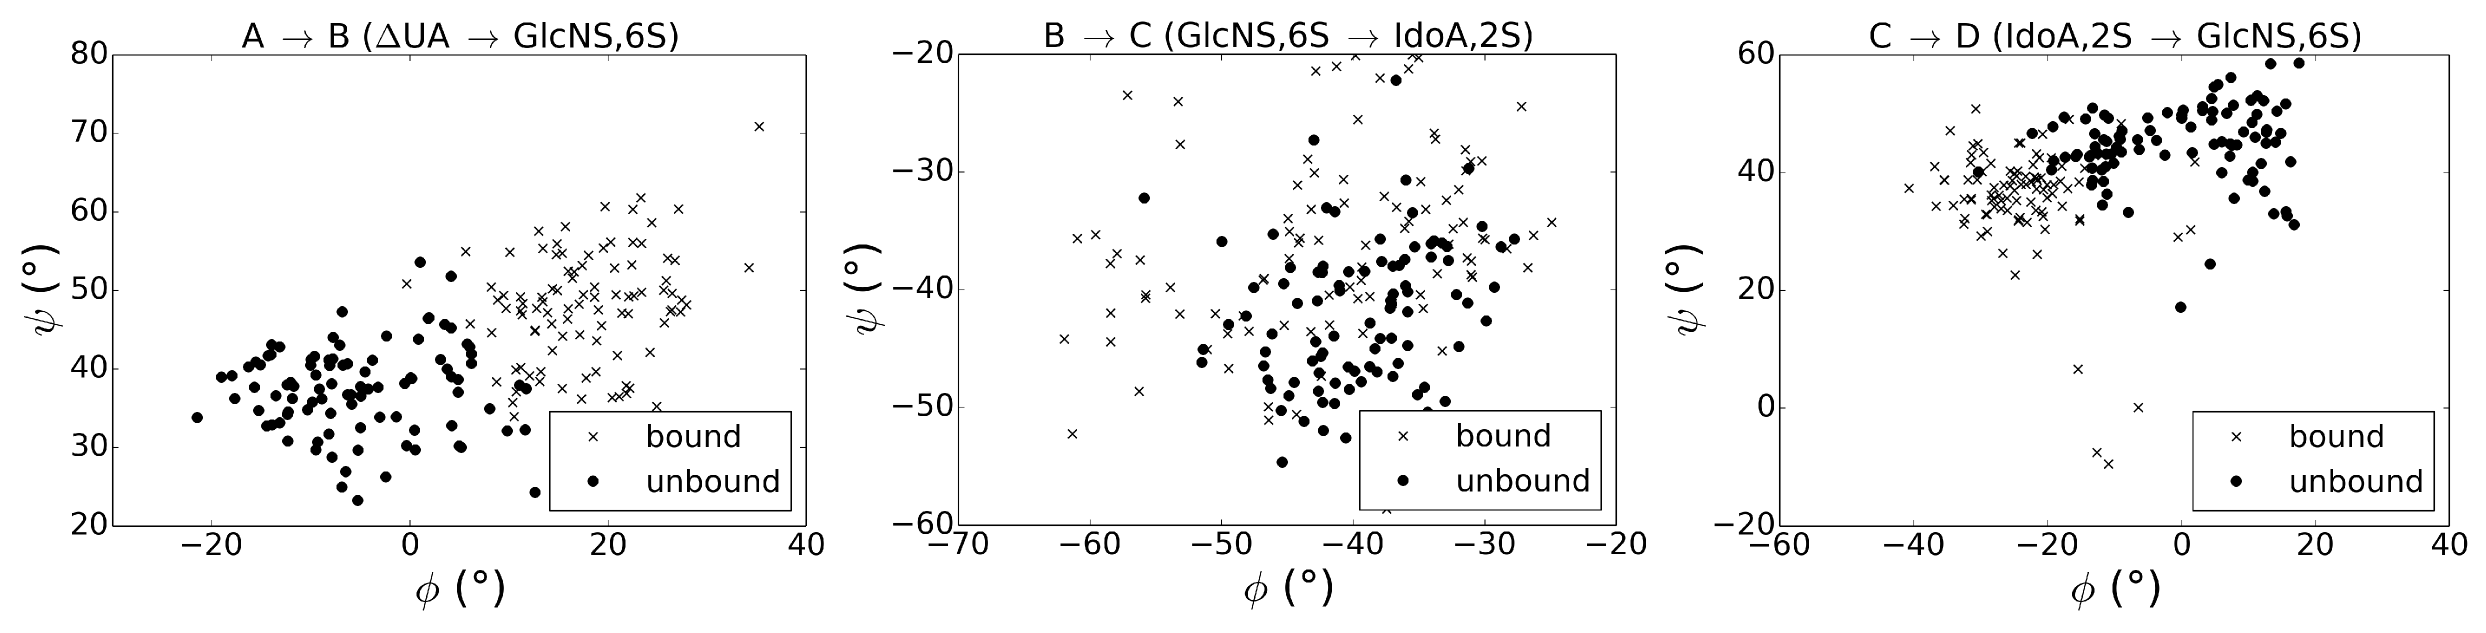
\includegraphics[width=1.3\textwidth]{gfx/nmr/Figure_08_glycolinkage_dihedrals_bound_vs_free_three_3panels_05.png}
\caption[]{
Glycosidic linkage torsional angle distributions of heparin structure model
ensembles obtained from NMR distance restraints and simulated annealing
simulations. Data comparing the bound and unbound state is shown individually
for each linkage in the heparin tetrasaccharide, namely for linkages A
\rightarrow B, B \rightarrow C, and C \rightarrow D.
}
\label{fig:nmr:hp_glyco_dihedral_distributions}
\end{adjustwidth}
\end{figure}

The orientation of four of the six sulfate groups in the tetrasaccharide did not
differ significantly between the bound and unbound state. The orientation of the
6-O-sulfates of the rings B and D, however, was observed to be affected by the
presence of IL-10 (see \cref{fig:nmr:hp_sulfate_orientations}). The 6-O-sulfate
of ring B showed a shift in the rotamer distribution and \SI{10}{\degree}
deviation from the ideal rotation angle of \SI{-60}{\degree}. The 6-O-sulfate of
ring D also populated a small fraction of the \textit{gauche-trans} conformer
(\SI{60}{\degree}) in the presence of IL-10. Further information on the
conformation of 6-O-sulfate side chains was revealed from 3J couplings between
H5 and H6 protons, \hl{as discussed in part...}

\begin{figure}
\centering
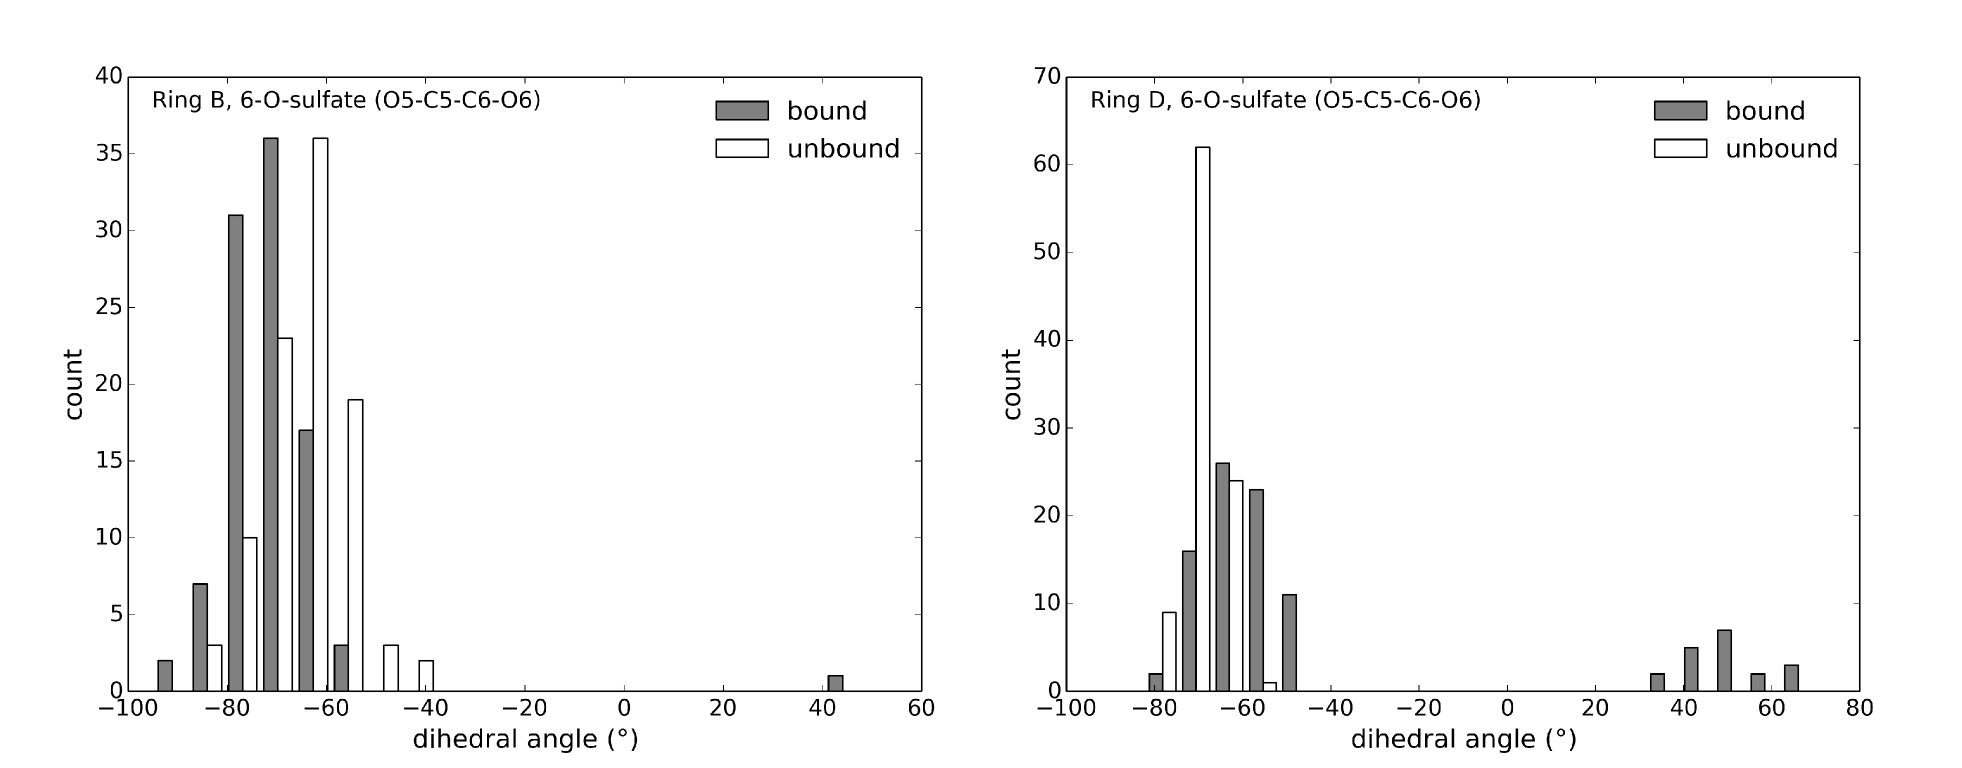
\includegraphics[width=\textwidth]{gfx/nmr/SI_figure_6O_sulfate_dihedrals_B_D_01.png}
\caption[]{
Distribution of 6-O-sulfate orientations in heparin tetrasaccharide structure
models obtained from H-H NMR distance restraints and simulated annealing
simulations, in comparison for the bound and unbound state.
}
\label{fig:nmr:hp_sulfate_orientations}
\end{figure}

The NOE distance data and MD simulations have led to proper heparin structure
models. In both, the bound and unbound case, the ensemble representatives have
their rings in valid conformations, namely ring B in ${}^4$C${}_1$, ring C in
${}^2$S${}_O$, and ring D in ${}^4$C${}_1$ conformation. Also the distribution
of glycosidic linkage torsional angles is in a valid range of values, as
observed in free heparin microsecond MD simulations (data not shown) and in
bound and unbound heparin structures found in the PDB.

The generated structure models let us conclude that the bound heparin structure
is less bent than its free form. The small but significant difference observed
in the backbone structure of the bound and unbound ensembles is reflected by
their glycosidic linkage torsional angle distributions. However, although
glycosidic bond angles between the free and bound state do vary between
\SI{10}{\degree} and \SI{30}{\degree} for linkages A→B and C→D, the overall
tetrasaccharide conformation is maintained and is consistent with the helical
structure of the heparin dodecasaccharide previously observed by NMR and
modelling \cite{foster_mulloy_1993}. Also in the high affinity complex between
bFGF and a heparin tetrasaccharide
\cite{faham_heparin_1996,mikhailov_hp_tetra_1996} the backbone differences
relative to the unbound GAG are rather small and provide no indication about the
interaction strength. Furthermore, according to our heparin structure models,
the orientation of most functional groups of rings B, C, and D is conserved
among the bound and unbound MD ensembles. Notable exceptions are the positions
of the 6-O-sulfate groups of ring B and D. In ring B the 6-O-sulfate is only in
\textit{gauche-gauche}, but there is a slight shift by about \SI{-10}{\degree}
of the rotamer distribution in the bound heparin structure. In ring C an
additional fraction of the \textit {gauche-trans} conformer in the presence of
IL-10 is observed. The observation of the 6-O-sulfate being mostly in \textit
{gauche-gauche} orientation is in contradiction to our \hl{3J} coupling
analysis. The latter estimated the C5-C6 bond in both glucosamine residues to
have \SI{70}{\percent} \textit{gauche- gauche} and \SI{30}{\percent} \textit
{gauche-trans} character as found for other D-glucopyranoses (Nishida et al.
1988). The described contradiction suggests that the sulfate rotamer
distribution as yielded by our MD structure optimization protocol is over-
sensitive to small variations in single distance restraints and that the
interpretation of the 3J coupling data should take precedence.

\hl{Note (TODO):}
\hl{Discuss what this HEPARIN STRUCTURE now brings us for clarifying atomic
detail interaction..}


\section{IL-10-GAG interaction enlightened via NMR}
\hl{Note (TODO):}
\hl{A summary of the remaining major results of Georg's NMR study.}


In \cref{chapter:bspred} we calculated IL-10's Coulomb potential and evaluated
its topology in space, and came up with a putative IL-10-GAG binding region. For
symmetry reasons, this region occurs twice in the IL-10 dimer, separated by a
distance of approximately 30 to 40 Å that is comparable to the length of an
extended GAG decasaccharide. Based on our STD binding data, we hypothesize a
scenario in which an appropriately long GAG molecule could bridge both binding
sites. For a fully sulfated heparin octa- or decasaccharide binding affinity is
nearly 10 or 20-fold higher than for the heparin disaccharide I-S. We interpret
this increase in affinity as effect of positive cooperativity indicated by a
steeper slope of the corresponding binding curves and a Hill coefficient of
around 2. Once the GAG molecule is fixed to one binding site, association with
the second site can happen very fast e.g. due to spatial restriction and thus
affinity is also increased.

\hl{Note (TODO):}
More discussion.
% That discrepancy probably originates from the strong H2-H5 NOE, which is
% dominated by the shorter H2-H5 distance of the 2SO structure (2.4 Å) compared to
% the 1C4 form (4.0 Å) (Mulloy et al. 1993) and thus fixes the monosaccharide in
% skew-boat-conformation during the simulation. In contrast, based on 3J couplings
% we determined the equilibrium between 1C4 and 2So in the IL-10-bound structure
% to be 33 %:67 %. This interesting observation can indicate that either the
% iduronic acid is not interacting with the protein, and thus interconversion of
% the sugar ring can take place, or that two binding modes may exist – one

% with the iduronic acid bound in 1C4 and the other with the iduronate in 2So. For
% some heparinprotein complexes also a conformational selection mechanism has been
% previously suggested. For example, in the crystal structure of annexin V with
% two heparin tetrasaccharide molecules the IdoA,2S ring of molecule 2, which
% interacts with the protein, adopts a 2So conformation whereas the non-
% interacting IdoA,2S ring in the second molecule resides in the 1C4 conformation
% (Capila et al. 2001). Furthermore, for the heparin pentasaccharide AGA*IA(M)
% (GlcNS,6S-GlcA-GlcNS,3S,6S-IdoA,2S-GlcNS,6S-Me) in complex with the FGF-receptor
% 2 (FGFR2) only the 2So conformer of IdoA was observed with NMR as a result of
% conformational selection (Nieto et al. 2011).

% In conclusion, we show that IL-10 is capable of binding a variety of GAG ligands
% for which we delimited their binding epitopes. This molecular recognition
% imposes only minor changes on the overall GAG structure. We find that the
% interaction strength is highly dependent on GAG sulfation, in particular
% N-sulfation. Our results provide information on the interaction properties of
% GAGs and IL-10 that can be taken into account e.g. for the design of tissue-like
% matrix materials in regenerative medicine.

% \section{Binding site determination via Pseudo Contact Shift measurements}
% \hl{Should this be in the thesis? Maybe ONLY prediction would be better,
% leave this for publication.}

%\lipsum[1-5]
\chapter{Bringing pieces together: the biological role of IL-10-GAG interaction}

In this short chapter, I assemble important insights about the IL-10-GAG system
derived during this thesis project and try to bring them into the biological
context. Some of these insights have a synergy effect, i.e.\ they support each
other and provide rather strong clues about how the IL-10-GAG system behaves in
nature on the molecular level.


\subsubsection{Experimental input: non-random, but weak interaction}

As noted in \cref{chapter:nmr}, our collaborators in Prof. Huster's NMR
laboratory at the University Leipzig could confirm binding between heparin
oligosaccharides and murine IL-10. As of the high similarity between human and
murine IL-10 (see \cref{background:il10biologyprimer}), this result is very
likely transferable between species. As published \cite{kuenze_gehrcke_2014},
the binding affinity between IL-10 and HP oligosaccharides measured in G.
Künze's NMR essays was determined to be in the micromolar range, whereas
Salek-Ardakini et al.\ found a binding affinity in the nanomolar range
\cite{salek_ardakani_2000}. Considering the differences in the investigated
systems (polymeric HP \textit{versus} oligomeric HP, human IL-10 \textit{versus}
murine IL-10) and the entirely different experimental techniques, it is no
worrying contradiction that both results differ by an order of magnitude.

The experimentally obtained binding affinity results and the computationally
obtained observation that IL-10-HP interaction has a measurable impact on the
backbone structure of HP (see \cref{chapter:nmr}) are strong clues that IL-10
and HP interact in a non-random fashion. However, various indicators point
towards a rather weak interaction, compared to e.g.\ FGF2-HP. One of these
pointers is that HP dp4's iduronic acid populates both, the ${}^1$C${}_4$ and
${}^2$S${}_\mathrm{O}$ conformations in the bound state (see
\cref{chapter:nmr}).


\subsubsection{Putative binding poses fit experimental data}

In \cref{chapter:bspred}, a putative IL-10-GAG binding region (occurring twice
as of the symmetry of the IL-10 homodimer) has been proposed, based on the
analysis of IL-10's Coulomb potential. In \cref{chapter:dmd}, it is described
how this binding region was further analyzed with DMD, and narrowed down towards
single key amino acids (being most responsible for GAG binding) and towards two
principal putative GAG binding poses, named A and B (see
\cref{fig:dmdil10:2nd_stage_principal_poses}). These poses are in the
neighborhood of R107, which has been identified as especially important for GAG
binding, and have special relations to experimentally obtained data, as will be
described in the following paragraphs.

\begin{figure}
\centering
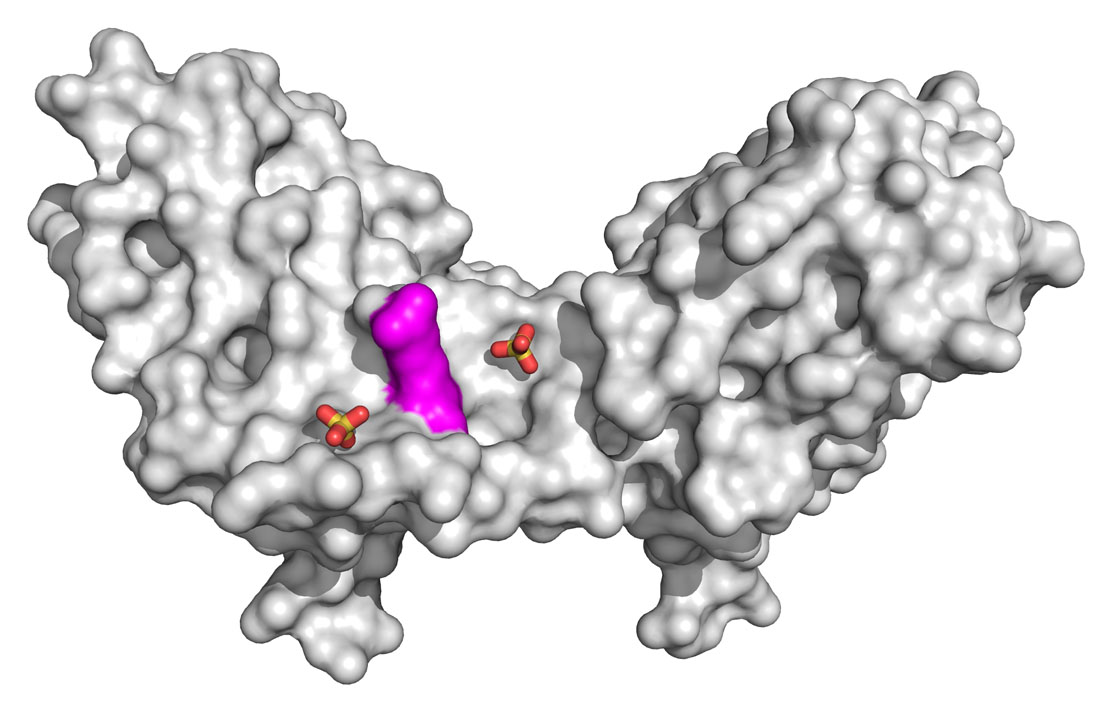
\includegraphics[width=1.0\textwidth]{gfx/together/il10sulfates_01.jpg}
\caption[]{
Structure of human IL-10 according to PDB entry 2ILK in surface representation,
including two sulfate groups contained in the crystal structure, shown in thick
stick representation. The surface of IL-10's amino acid residue R107 is colored
in magenta. During crystal growth, sulfate groups assume energetically favorable
positions, which are transferable to sulfate groups in GAGs.}
\label{fig:together:il10sulfates}
\end{figure}

In protein crystallization, salts are often used for diminishing the
electrostatic repulsion and for promoting the hydrophobic interactions among
proteins. In high-quality crystal structures, the atomic groups of salts are
spatially resolved and visible. Often, sulfates are used for facilitating the
crystal growth \cite{crystal_salts_2001}. During crystal growth, these atomic
groups end up in positions that are physically favorable for them and therefore
provide valuable input when it comes to the investigation of protein-GAG
interaction: it is valid to assume that the very same locations would also be
energetically favorable for sulfate groups contained in GAGs.

Three sulfate groups are contained in the 2ILK crystal structure of IL-10 (which
has been used throughout this thesis). Two of these sulfate groups are located
right in the neighborhood of R107, as shown in \cref{fig:together:il10sulfates}.
The location of the sulfate groups contained in the 2ILK crystal structure is a
strong experimental support of the the putative IL-10-GAG binding region
presented in \cref{chapter:bspred}. Furthermore, the imaginary line connecting
both sulfate groups aligns well with the putative GAG binding pose A that was
shown in \cref{fig:dmdil10:2nd_stage_principal_poses}. The putative GAG binding
pose B crosses the position of one of both sulfate groups.

As described in \cref{chapter:nmr}, NMR data suggests a cooperative binding mode
in which a GAG oligosaccharide bridges both symmetrically aligned putative
IL-10-GAG binding regions. In a thought experiment, extended versions of both
putative GAG binding poses, A and B, can be thought to connect both binding
regions on the front and back of the IL-10 V-shape. For binding mode B, however,
this seems to be a more probable scenario than for binding mode A.


\subsubsection{Scenario: modulation of IL-10 biology by impaired diffusion}

\begin{figure}
\centering
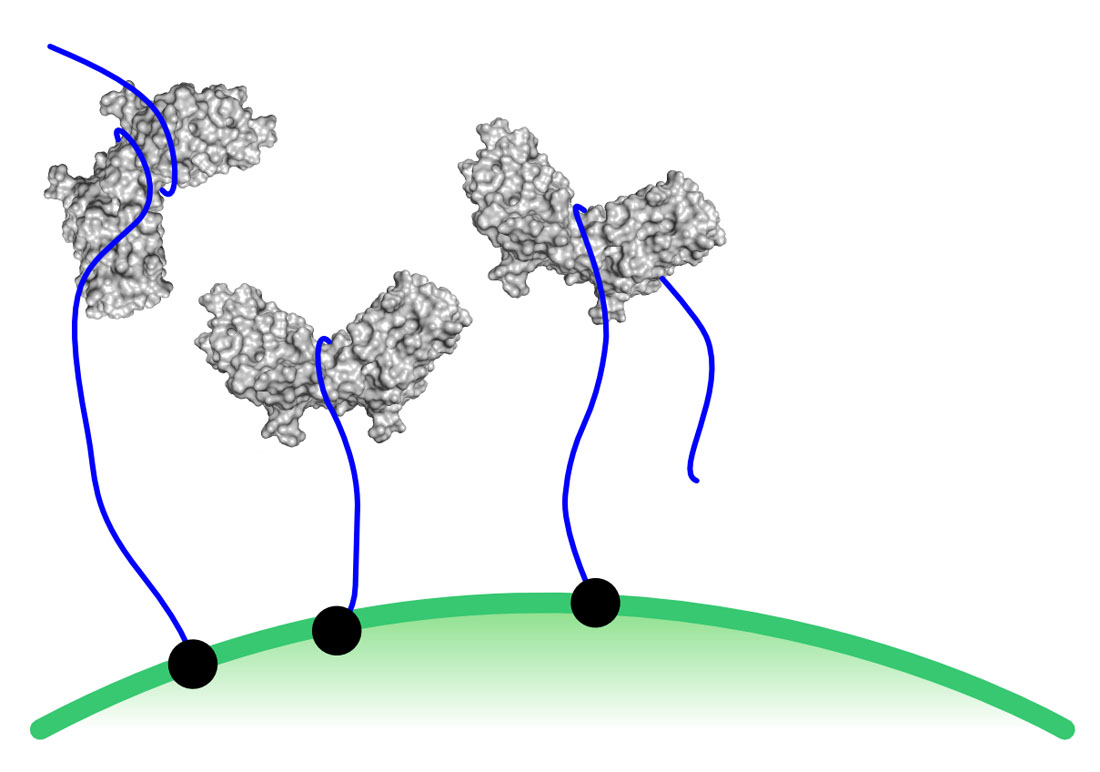
\includegraphics[width=1.0\textwidth]{gfx/together/agglomeration_small.jpg}
\caption[]{
Schematic visualization of how cell surface-attached proteoglycans (black) with
long GAG chains (blue) might impair IL-10 (gray) diffusion. The cell membrane is
here indicated in green, with the inner part of the cell being at the bottom.
The exact location and curvature of the GAG polysaccharides is not to be taken
literally.}
\label{fig:together:diffusionimpaired}
\end{figure}

In literature it is often speculated that cytokine-GAG interaction for certain
systems does not directly affect the signaling cascade, but rather may be a
mechanism for cytokine concentration and diffusion control, e.g.\ for retaining
a type of cytokine close to its site of secretion in the tissue (see
\cref{background}). The question after the biological meaning of IL-10-GAG
interaction could not be answered in this project. However, the scenario in
which longer GAG chains impair the diffusion of IL-10 without affecting the
IL-10 receptor system seems to be a valid model, after the findings made in this
thesis project.

Considering the IL-10 ternary complex model discussed in
\cref{background:structureil10system} and shown in
\cref{fig:bg:il10_il10r1_il10r2_model}, the interaction of IL-10 with its
receptors is focused towards the sides of IL-10's V-shape. The IL-10-GAG
interaction, however, is predicted to mainly occur in the groove of the V-shape,
especially regarding a potential cooperativeness of both symmetrically aligned
binding regions. It is therefore entirely conceivable that IL-10-GAG interaction
does \textit{not} affect the interaction between IL-10 and both of its
receptors. At the same time, a cooperative \enquote{attack} of a polymeric GAG
chain focused on the groove of the V would be an effective mechanism for
impairing the diffusion of the IL-10 homodimer, assuming that the GAG chain is
fixed on at least one side. This model would very well fit the idea of impaired
cytokine diffusion due to cell surface-attached proteoglycans, as schematically
depicted in \cref{fig:together:diffusionimpaired}.


\subsubsection{Scenario: modulation of IL-10 biology by interference with
receptor binding}

\begin{figure}
\centering
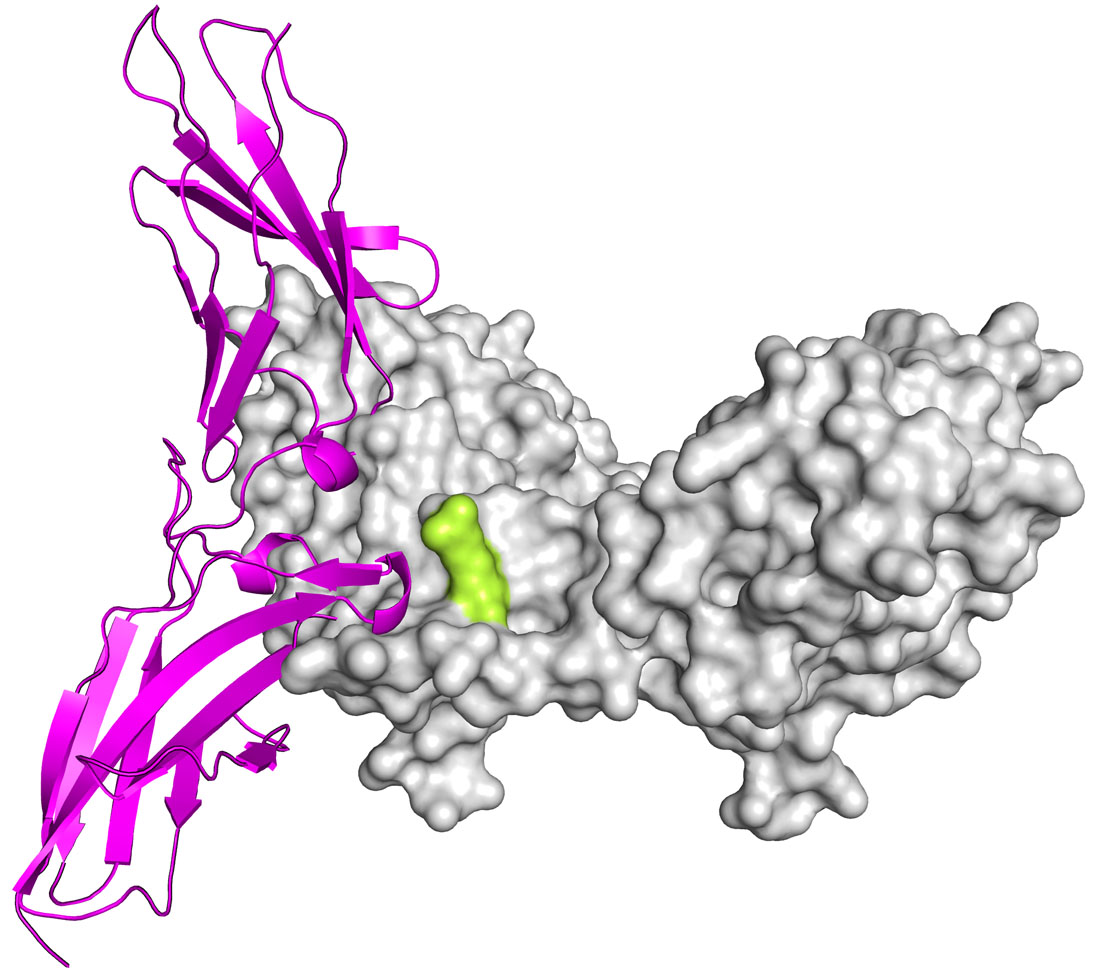
\includegraphics[width=1.0\textwidth]{gfx/together/il10dimer_surface_r2cartoon_r107_01.jpg}
\caption[]{
Binding model of IL-10R2 (magenta) and IL-10 (gray), with R107 highlighted in
yellow. The binding model has previously been described in
\cref{background:structureil10system} and shown in
\cref{fig:bg:il10_il10r1_il10r2_model}. Here, the close proximity between R107
to IL-10R2 is to be pointed out, which suggests a potential structural
interference between a GAG molecule bound near R107 on the one hand, and IL-10R2
on the other hand.}
\label{fig:together:r2impaired}
\end{figure}

While the above-presented scenario of a GAG-induced impaired IL-10 diffusion
fits the findings obtained in this thesis project quite well, a more direct
impact of GAG molecules on IL-10 biology via involvement in receptor binding
can not be excluded. Specifically, considering the ternary IL-10 complex
binding model as discussed in \cref{background:structureil10system} and shown in
\cref{fig:bg:il10_il10r1_il10r2_model}, IL-10R2 has contacts to IL-10 that
are potentially quite close to R107, see \cref{fig:together:r2impaired}. In this
model, it is conceivable that a GAG molecule bound in close proximity to R107
could at least sterically interact with IL-10R2, and potentially impede
formation of the ternary complex required for IL-10 signaling. The GAG molecule
would therefore have a direct impact on IL-10 biology. It should be stressed
that this scenario is speculative but allowed in the framework of the
information obtained about the IL-10-GAG system so far. Specifically, A GAG
bound in the principal binding mode A shown in
\cref{fig:dmdil10:2nd_stage_principal_poses} would interfere with IL-10R2,
according to this model.

Notably, no solid data has been obtained in the course of this project that
suggest that GAGs could interfere with the interaction between IL-10 and
IL-10R1.

\chapter{Conclusions}


- cooperative binding behavior
- binding in that region might affect R2 binding according to the model
    presented in ...






    - Insights for IL-10-GAG system
        - binding site
        - binding behavior (heparin, N sulfate, conformation, important residue)
        - binding implications




    - Methodological development
        - Binding site prediction
        - Clustering
        - DMD
        - Experimental setup: HPC, ZIH and group-internal


    no real binding specificity clarified, e.g. effect of N sulfation not clarified. this requires further in silico sampling techniques, and for the sake of creating reliable results, a clear and certain knowledge about the binding region / site (this is something for outlook). Also, further experimental data needs to be obtained, in vitro experiments, SPR with mutants, etc.


    Furthermore, K119 — which
was left undiscussed in chapter 2 — potentially plays an important
role, as it might cooperate with R107 in trapping a GAG from two
sides simultaneously. This structural model of IL-10-GAG interaction
is supported by clustering data that led to the observation of two
principally different GAG binding poses in the region of interest, both
heavily involving R107
%\chapter{Outlook}
\lipsum[1-10]


\backmatter
%\SingleSpacing
\begin{adjustwidth}{-1.5cm}{-1.5em}
\printbibliography
\end{adjustwidth}


% Some abbreviations, maybe put them into the document later.
\nomenclature{PDB}{RCSB Protein Data Bank}
\nomenclature{MD}{molecular dynamics}
\nomenclature{NOE}{nuclear Overhauser effect}
\nomenclature{NMR}{nuclear magnetic resonance}
\nomenclature{IL-10}{interleukin-10}
\nomenclature{ECM}{extracellular matrix}


% http://tex.stackexchange.com/a/100377
% http://www.latex-community.org/forum/viewtopic.php?f=47&t=19574
% Define "chapter name" for page headings, set it to current nomenclature name
% (nomname is defined by nomencl package, and can ge changed).
\markboth{\nomname}{\nomname}

% Print the nomencl list, with a certain spacing between abbreviation and
% explanation.
\printnomenclature[3cm]

%\OnehalfSpacing

\appendix
\appendixpage
%\addappheadtotoc


% Aus der Promotionsordnung:
% 5. eine Erklärung des Bewerbers zu folgenden Sachverhalten:
% a) eine Versicherung gemäß Anlage 1;
% b) wo und unter wessen wissenschaftlicher Betreuung die Dissertation
%    angefertigt wurde;

% Alle Unterlagen gemäß Nr. 1 - 8 sind in schriftlicher Form einzureichen und
% müssen vom Bewerber autorisiert oder amtlich beglaubigt sein. Die Erklärungen
% gemäß Nr. 5. a) und b) sind auf einem Blatt der Dissertation am Ende anzufügen
% und mit einzubinden.

\chapter{Erklärung gemäß § 5 der Promotionsordnung der TU Dresden}

Die Dissertation wurde unter der wissenschaftlichen Betreuung von Dr. M. Teresa
Pisabarro am BIOTEC (TU Dresden) in der Arbeitsgruppe Structural Bioinformatics
angefertigt.

Hiermit versichere ich, dass ich die vorliegende Arbeit ohne unzulässige Hilfe
Dritter und ohne Benutzung anderer als der angegebenen Hilfsmittel angefertigt
habe; die aus fremden Quellen direkt oder indirekt übernommenen Gedanken sind
als solche kenntlich gemacht. Die Arbeit wurde bisher weder im Inland noch im
Ausland in gleicher oder ähnlicher Form einer anderen Prüfungsbehörde vorgelegt.

\vspace{2cm}

\noindent
\namesigdate[6cm]{Jan-Philip Gehrcke}

\end{document}
